\documentclass[xcolor=dvipsnames,10pt]{beamer}
\usepackage[english]{babel}
\usepackage[utf8]{inputenc}
\usepackage{pict2e}
\usepackage{colortbl}
\usepackage{graphicx}
\usepackage{pdfpages}
\usepackage{verbatim}
\usepackage{pgf}
%%%%%%%%%%%%%%%%%%%%
%%% nice math
\usepackage{amssymb}
\usepackage{amsmath}
\usepackage{latexsym}
\usepackage{amsthm}
\usepackage{slashed}
%%%%%%%%%%%%%%%%%%%%
%%% font type
%\usepackage{times}
\usepackage{bookman}
%\usepackage{palatino}
%\usepackage{newcent}
%\usepackage{avant}
\usefonttheme{serif}
\usepackage{atlasphysics}
%\usepackage{tikz}
\usepackage{subfigure}
\usepackage{tikz}

\newcommand{\Simley}[1]{%
\begin{tikzpicture}[scale=0.11]
    \newcommand*{\SmileyRadius}{1.0}%
    \draw [draw=MidnightBlue] (0,0) circle (\SmileyRadius)% outside circle
        %node [yshift=-0.22*\SmileyRadius cm] {\tiny #1}% uncomment this to see the smile factor
        ;  

    \pgfmathsetmacro{\eyeX}{0.5*\SmileyRadius*cos(30)}
    \pgfmathsetmacro{\eyeY}{0.5*\SmileyRadius*sin(30)}
    \draw [fill=MidnightBlue,draw=none] (\eyeX,\eyeY) circle (0.15cm);
    \draw [fill=MidnightBlue,draw=none] (-\eyeX,\eyeY) circle (0.15cm);

    \pgfmathsetmacro{\xScale}{2*\eyeX/180}
    \pgfmathsetmacro{\yScale}{1.0*\eyeY}
    \draw[color=MidnightBlue, domain=-\eyeX:\eyeX]   
        plot ({\x},{
            -0.1+#1*0.15 % shift the smiley as smile decreases
            -#1*1.75*\yScale*(sin((\x+\eyeX)/\xScale))-\eyeY});
\end{tikzpicture}%
}%



\newcommand{\AC}{\ensuremath{\text{A}_{\text{C}}}}
\newcommand{\formatGenerator}[1]{\textsc{#1}}
\newcommand{\mcnlo}{\formatGenerator{mc@nlo}}
\newcommand{\wjets}{\ensuremath{W+\mathrm{jets}}}
\providecommand{\abs}[1]{\lvert#1\rvert}
\newcommand{\dy}{\ensuremath{\Delta{}\abs{y}}}
\newcommand{\deta}{\ensuremath{\Delta{}\abs{\eta}}}
\newcommand{\mtt}{\ensuremath{m_{\ttbar{}}}}
\newcommand{\Nupup}{\ensuremath{N(\uparrow\uparrow)}}
\newcommand{\Ndodo}{\ensuremath{N(\downarrow\downarrow)}}
\newcommand{\Nupdo}{\ensuremath{N(\uparrow\downarrow)}}
\newcommand{\Ndoup}{\ensuremath{N(\downarrow\uparrow)}}


\newcommand\myskip{\vspace{\baselineskip}}
\def\Xbar{\ensuremath{\bar{X}}}
\def\XXbar{\antibar{X}}
\def\Ybar{\ensuremath{\bar{Y}}}
\def\YYbar{\antibar{Y}}
\def\Tbar{\ensuremath{\bar{T}}}
\def\TTbar{\antibar{T}}
\def\Bbar{\ensuremath{\bar{B}}}
\def\BBbar{\antibar{B}}
\newcommand\TT{\ensuremath{T\bar{T}}}
\newcommand\BB{\ensuremath{B\bar{B}}}
\newcommand\T{\ensuremath{T}}
\newcommand\B{\ensuremath{B}}
\newcommand{\TB}{\ensuremath{(T \, B)}}
\newcommand{\XT}{\ensuremath{(X \, T)}}
\newcommand{\BY}{\ensuremath{(B \, Y)}}
\def\Tlr{\ensuremath{T_{L,R}}}
\def\Blr{\ensuremath{B_{L,R}}}
\def\Ylr{\ensuremath{Y_{L,R}}}
\def\Xlr{\ensuremath{X_{L,R}}}
\def\TBlr{\ensuremath{\TB_{L,R}}}
\def\BYlr{\ensuremath{\BY_{L,R}}}
\def\XTlr{\ensuremath{\XT_{L,R}}}
\def\vlt{vector-like top partner}
\def\vlb{vector-like bottom partner}

%%%%%%%%%%%%%%%%%%%%%%%%
%%% LAZYNESS-DRIVEN DEFS
%%%%%%%%%%%%%%%%%%%%%%%%
\def\cme{center-of-mass energy}
\def\cmm2{cm$^{-2}$}
\def\sm1{s$^{-1}$}
\def\chisq{$\chi^2$}
\def\loose{{\sc Loose}}
\def\tight{{\sc Tight}}
\def\whad{\ensuremath{W_{\rm had}}}
\def\wlep{\ensuremath{W_{\rm lep}}}
\def\wi{$W_{\rm had}^{\rm type\;I}$}
\def\wii{$W_{\rm had}^{\rm type\;II}$}
\def\mreco{\ensuremath{m_{\rm reco}}}
\def\chii{{\sc ``{\small 2 \btag ged jets}''}}
\def\chiii{{\sc ``{\small 3 \btag ged jets}''}}
\def\chiv{{\sc ``{\small{\footnotesize$\geq$}4 \btag ged jets}''}}

\def\dr{\ensuremath{\Delta R}}
\def\OR{\texttt{OR}}
\def\AND{\texttt{AND}}
%\def\bjet{$b$jet}
\def\bjet{$b$-jet}
%\def\cjet{$c$jet}
\def\cjet{$c$-jet}
\def\ljet{light-jet}
\def\btag{$b$-tag}
\def\ctag{$c$-tag}
\def\mt{\ensuremath{m_T}}
\def\mtw{\ensuremath{m_T(W)}}
\def\wbx{\ensuremath{\TTbar\to Wb+X}}
\def\htx{\ensuremath{\TTbar\to Ht+X}}
\def\nontt{non-$t\bar{t}$}
\def\mclimit{\texttt{MCLimit}}
\def\cls#1{\ensuremath{CL_{\rm #1}}}
\def\hthad{\ensuremath{H_T^{\rm had}}}
\def\htfj{\ensuremath{H_T^{4j}}}
\def\tthf{\ttbar+HF}
\def\ttlf{\ttbar+light}

\def\bra#1{\mathinner{\langle{#1}|}}
\def\ket#1{\mathinner{|{#1}\rangle}}
\def\braket#1{\mathinner{\langle{#1}\rangle}}
\def\Bra#1{\left<#1\right|}
\def\Ket#1{\left|#1\right>} 
\newcommand{\Overline}[2][1]{%
  {}\mkern#1mu \overline{\mkern-#1mu #2 \mkern-#1mu}\mkern#1mu {}} 
\DeclareMathAlphabet{\mathpzc}{OT1}{pzc}{m}{it}



%%% nice tables
\usepackage{booktabs}
\usepackage{multirow,bigdelim}
\usepackage{dcolumn}

\usepackage{fancybox}

%%% code pieces
\usepackage{listings}
\lstset{basicstyle=\tiny,language=c,emphstyle=\color{red},columns=fullflexible,
keepspaces=false, keywordstyle=\tiny\color{blue}, showstringspace=false} 
\newcommand\BackgroundPicture[1]{%
   \setbeamertemplate{background}{%
   \parbox[c][\paperheight]{\paperwidth}{%
       \vfill \hfill
\includegraphics[width=0.6\paperwidth,height=0.6\paperheight]{#1}
        \hfill \vfill
     }}}
\newcommand\FullBackgroundPicture[1]{%
   \setbeamertemplate{background}{%
   \parbox[c][\paperheight]{\paperwidth}{%
     \centering\vspace{2cm} \vfill 
\includegraphics[width=0.8\paperwidth,height=0.7\paperheight]{#1}
\vfill 
     }}}

%\setbeamertemplate{headline}

%%% to allow small margin
\newenvironment{changemargin}[2]{%
  \begin{list}{}{%
    \setlength{\topsep}{0pt}%
    \setlength{\leftmargin}{#1}%
    \setlength{\rightmargin}{#2}%
    \setlength{\listparindent}{\parindent}%
    \setlength{\itemindent}{\parindent}%
    \setlength{\parsep}{\parskip}%
  }%
  \item[]}{\end{list}} 

%\usetheme{Luebeck}
%\usecolortheme{seagull}
%\usecolortheme[named=BrickRed]{structure}


\usetheme[headheight=.13\textheight,footheight=.035\textheight]{boxes}
\definecolor{light-gray}{gray}{0.9}
%\definecolor{myfading}{fg=white,bg=light-gray}
\definecolor{structure2}{rgb}{1,1,1}

\mode<presentation>
%\usecolortheme[named=Black]{structure}
%\usecolortheme[named=Plum]{structure}
%\usecolortheme[named=Violet]{structure}
%\usecolortheme[named=BurntOrange]{structure}
%\usecolortheme[named=RedViolet]{structure}
\usecolortheme[named=MidnightBlue]{structure}
%\usecolortheme[named=Sepia]{structure}
\setbeamercolor{normal text}{fg=black!70!light-gray,bg=white}
\setbeamercolor{alerted text}{fg=BrickRed,bg=light-gray}
\setbeamercolor{boxcolor}{fg=black!70!light-gray,bg=structure!30!white}
\setbeamercolor{whiteboxcolor}{fg=black!70!light-gray,bg=white}

\definecolor{links}{named}{Plum}

\usepackage{hyperref}
\hypersetup{colorlinks=true,linkcolor=,urlcolor=links}

\setbeamercolor{head/foot boxes}{fg=structure!90!white,bg=structure!30!white}
\setbeamercolor{head/foot boxes bis}{fg=structure!60!white,bg=structure!90!white}

\setbeamercolor{head/foot text}{fg=structure!40!black,bg=structure!30!white}

%\addheadboxtemplate{\usebeamercolor[bg]{head/foot boxes}}{\usebeamercolor[fg]{head/foot text}\logo{
\includegraphics[height=1.2cm]{pics/atlasifae2}}\raisebox{-1.8ex}{\insertlogo}\hfill\insertshorttitle \hskip0.3cm}
\addheadboxtemplate{\usebeamercolor[bg]{head/foot boxes}}{\usebeamercolor[fg]{head/foot text}\insertsubsectionhead \hskip0.3cm}
\addheadboxtemplate{\usebeamercolor[fg]{head/foot boxes}}{\usebeamercolor[bg]{head/foot text}\scriptsize\hskip0.3cm\insertsectionhead}

\addfootboxtemplate{\usebeamercolor[fg]{head/foot boxes}}{\usebeamercolor[bg]{head/foot text}\hskip0.3cm\insertshortauthor\\\insertshortinstitute \hfill}
\addfootboxtemplate{\usebeamercolor[fg]{head/foot boxes bis}}{\usebeamercolor[fg]{head/foot text}\hfill\insertdate\hfill}

\def\insertpresentationendframe{\inserttotalframenumber}
\makeatletter
\g@addto@macro{\appendix}{\immediate\write\@auxout{\string\@writefile{nav}{\noexpand\headcommand{\noexpand\def\noexpand\insertpresentationendframe{\the\c@framenumber}}}}}
\makeatother

\addfootboxtemplate{\usebeamercolor[bg]{head/foot boxes}}{\usebeamercolor[fg]{head/foot text}\hfill\insertframenumber/\insertpresentationendframe\hskip0.3cm}
%\addfootboxtemplate{\usebeamercolor[bg]{head/foot boxes}}{\usebeamercolor[fg]{head/foot text}\hfill\insertframenumber/\insertpresentationendpage\hskip0.3cm}

%\setbeamertemplate{footline}{%
%  \begin{beamercolorbox}{section in head/foot}
%\begin{center}
%\begin{tabular}{lcr}
%\hskip45pt \textit{Barcelona plans for u4u4 searches in lepton+jets} \phantom{a/aa} & 2011, December 21st \phantom{a/aa} \insertframenumber / %\insertpresentationendpage
%\\
%\end{tabular}
%\end{center}  \end{beamercolorbox}
%}


%\usesectionheadtemplate
%{\color{white}\tiny\textbf{\insertsectionhead}}
%{\color{structureshaded}\tiny\textbf{\insertsectionhead}}


%\useoutertheme{sidebar}
%\setbeamertemplate{sidebar canvas left}[vertical shading][top=White,bottom=Gray]
%\setbeamertemplate{sidebar canvas left}[vertical shading][top=White,bottom=CadetBlue]
%\setbeamertemplate{sidebar canvas left}[vertical shading][top=White,bottom=YellowGreen]
%\setbeamertemplate{sidebar canvas left}[vertical shading][top=White,bottom=light-gray]

\setbeamertemplate{navigation symbols}{}
\setbeamersize{text margin left=.2cm,text margin right=.2cm} 






\AtBeginSection[]
{
  \begin{frame}\centering
    \frametitle{Outline}
    \tableofcontents[currentsection]
  \end{frame}
}



\title[Probing new physics at the LHC: \\ searches for heavy top-like quarks \\ with the ATLAS experiment]{{\bfseries Probing new physics at the LHC: \\ searches for heavy top-like quarks \\ with the ATLAS experiment}}
\author[A Succurro]{Antonella Succurro\\ \vspace{\baselineskip}\textit{\small PhD candidate in Physics}\vspace{-0.7cm}}
\institute[\, \emph{IFAE, UAB}]{
\begin{tabular}{p{0.25\textwidth} p{0.25\textwidth} p{0.25\textwidth}}
  \vspace{0.7cm} 
\includegraphics[width=2.5cm]{../smallstuff/ifae_logo.pdf}\hspace{0.2cm}&
  \vspace{0.5cm} 
\includegraphics[width=2.8cm]{../smallstuff/uab_logo.pdf}&
  \vspace{0.cm} \hspace{0.5cm} 
\includegraphics[width=1.5cm]{pics/atlas_logo}\\
\end{tabular}
}
\date{Bellaterra, 28th of February, 2014}

\definecolor{LightCyan}{rgb}{0.88,1,1}
\definecolor{TabLight}{rgb}{0.53,0.81,0.92}
\def\cccolor{\usebeamercolor[fg]{head/foot boxes}}

\def\pchii{{\sc ``{2 \btag ged jets}''}}
\def\pchiii{{\sc ``{3 \btag ged jets}''}}
\def\pchiv{{\sc ``{$\geq$4 \btag ged jets}''}}


\begin{document}


\frame{

\vspace{-.8cm}

\maketitle\centering

\vspace{-.8cm}
}



\begin{frame}\frametitle{Four questions, one dissertation}

%{\large\bfseries
%\usebeamercolor[fg]{head/foot boxes}
%\dots one thesis\dots
%}

%\myskip

%\pause
\centering
  \begin{minipage}{.5\textwidth}\centering

%\myskip

\begin{itemize}[<+->]
\item {\cccolor \LARGE Why?} {\scriptsize bother with ``new physics''}
\item {\cccolor \LARGE Where?} {\scriptsize is all happening}
\item {\cccolor \LARGE What?} {\scriptsize are we looking at}
\item {\cccolor \huge How?} {\scriptsize}
\end{itemize}

\end{minipage}

%\pause
%\flushright
%{\large\bfseries
%\usebeamercolor[fg]{head/foot boxes}
%\dots no solution! (yet)
%}


\end{frame}

%\begin{frame}\frametitle{Content}
%\end{frame}
%\begin{frame}\frametitle{Outline}
%\centering
%\tableofcontents[part=1,pausesections]
%\tableofcontents
%\end{frame}

%----------------------------------
%\section{Introduction}
%----------------------------------
%\begin{frame}\frametitle{Standard Model as an effective theory}
%\scriptsize\centering
%\end{frame}


%----------------------------------
\section{Theoretical framework}
%----------------------------------

\begin{frame}\frametitle{A successfull theory}
\scriptsize\centering

\begin{minipage}{.55\textwidth}\centering

\resizebox{1.\textwidth}{!}{\tiny
\begin{tabular}{c x{.12\textwidth} x{.12\textwidth} x{.12\textwidth} x{.12\textwidth}}\toprule
Fermions   & \multicolumn{2}{c}{Leptons}&\multicolumn{2}{c}{Quarks} \\ 
generation & $q=-1$ & $q=0$ &$q=\frac{2}{3}$ &$q=-\frac{1}{3}$ \\ \midrule
I & $e^{-}$ & $\nu_{e}$ & $u$ & $d$ \\
II & $\mu^{-}$ & $\nu_{\mu}$ & $c$ & $s$ \\
III & $\tau^{-}$ & $\nu_{\tau}$ & $t$ & $b$ \\ \midrule%\bottomrule\toprule
Force & Electromagnetic &\multicolumn{2}{c}{Weak}& Strong\\\midrule
Carrier boson & $\gamma$ & $W^{\pm}$ &$Z$ & $g$\\
spin & 1 & 1 &  1 & 1 \\
$q$ & 0 & $\pm$1 & 0 & 0\\ \midrule%\bottomrule\toprule
 \multicolumn{2}{c}{Higgs boson $H$}& \multicolumn{3}{c}{$q=0$, spin=0} \\
\bottomrule
\end{tabular}
}

\begin{pgfpicture}{0.0\textwidth}{0.0\textheight}{1.\textwidth}{.5\textwidth}

\begin{pgfscope}
\pgfdeclareimage[interpolate=true,width=.75\textwidth]{wtop}{pics/W_vs_top}
\pgfputat{\pgfxy(.8,-0.2)}{\pgfbox[left,base]{\pgfuseimage{wtop}}}
 \pgfsetlinewidth{1.pt}
 \usebeamercolor[fg]{head/foot boxes}
\only<2>{
 \pgfrect[stroke]{\pgfxy(2,5.48)}{\pgfxy(1.7,0.57)}
 \begin{pgfrotateby}{\pgfdegree{30}}
 \pgfputat{\pgfxy(3.,4.3)}{\pgfbox[left,base]{\scriptsize\bf\begin{tabular}{c} ``who ordered\\ that??''\\\tiny [I.I.Rabi]\\\end{tabular}}}
 \end{pgfrotateby}
}
\only<3>{
 \pgfrect[stroke]{\pgfxy(4.6,5.75)}{\pgfxy(1.7,0.3)}
}
 \usebeamercolor[bg]{head/foot boxes}
 \pgfsetlinewidth{.7pt}
\only<4>{
\pgfline{\pgfxy(4.85,5.3)}{\pgfxy(5.,2.3)}
\pgfline{\pgfxy(3.6,4.4)}{\pgfxy(5.,2.3)}
}
\only<5>{
\pgfline{\pgfxy(4.85,5.3)}{\pgfxy(4.5,2.3)}
\pgfline{\pgfxy(3.6,4.4)}{\pgfxy(4.5,2.3)}
\pgfline{\pgfxy(2.2,3.6)}{\pgfxy(4.5,2.3)}
}

\end{pgfscope}
\end{pgfpicture}

%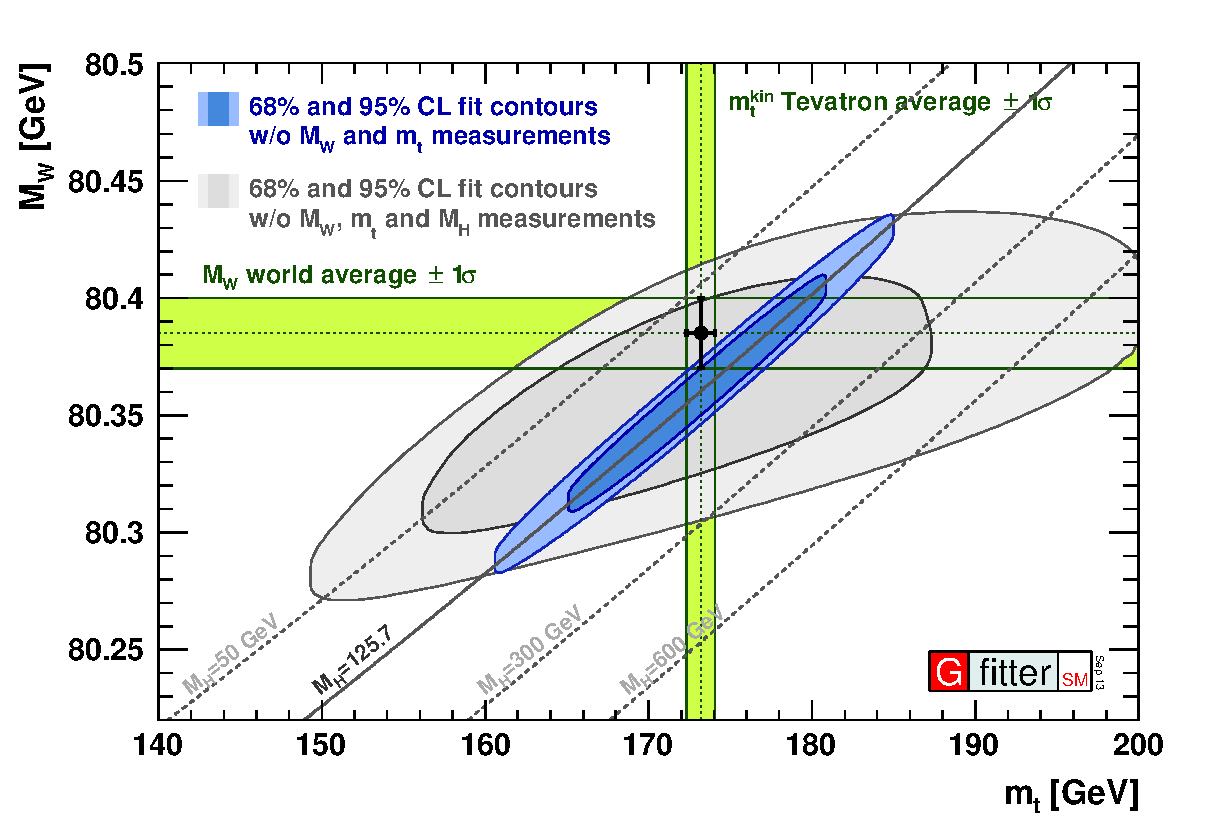
\includegraphics[width=0.8\textwidth]{pics/W_vs_top}


\end{minipage}\begin{minipage}{.45\textwidth}\centering

\vskip-5ex
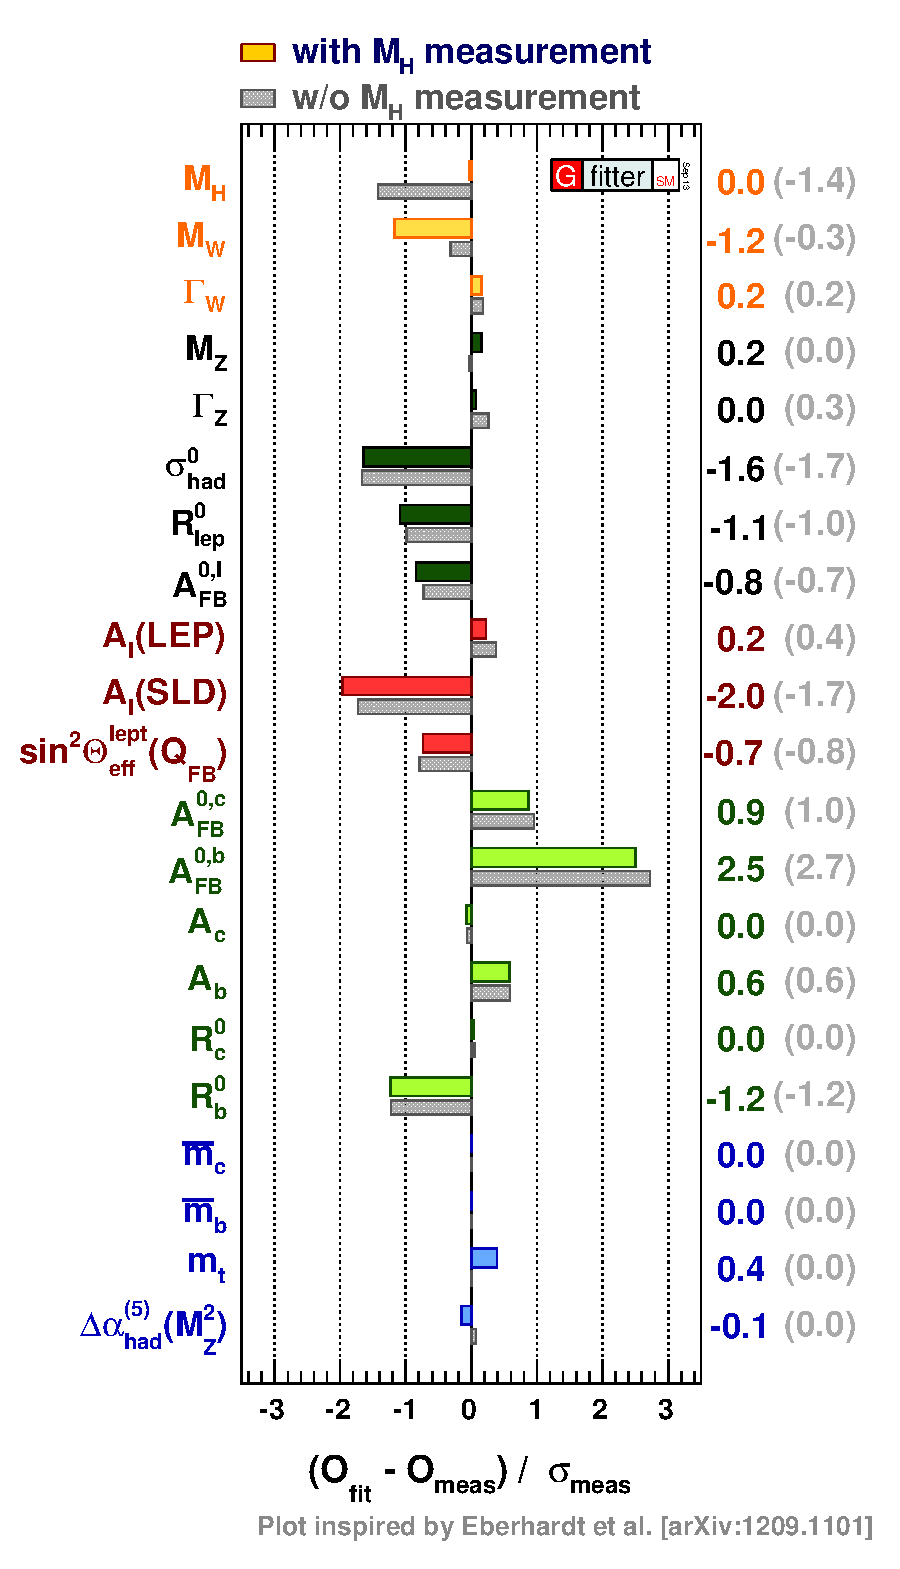
\includegraphics[width=0.8\textwidth]{pics/fitSM_new}

\end{minipage}\end{frame}


\begin{frame}\frametitle{\dots effectively}
\scriptsize\centering

\begin{pgfpicture}{0.0\textwidth}{0.0\textheight}{1.\textwidth}{.6\textwidth}

\begin{pgfscope}
\pgfdeclareimage[interpolate=true,width=.4\textwidth]{pie}{pics/piematter}
\pgfdeclareimage[interpolate=true,width=.42\textwidth]{gut}{pics/gut}
\pgfdeclareimage[interpolate=true,width=.3\textwidth]{loop}{pics/loop1}
\onslide<1->{
\pgfputat{\pgfxy(0.5,0.1)}{\pgfbox[left,base]{\pgfuseimage{gut}}}
\pgfputat{\pgfxy(3.,2.1)}{\pgfbox[left,base]{\small \bf\cccolor GUT theories? Gravity?}}
\pgfputat{\pgfxy(7.,3.6)}{\pgfbox[left,base]{\pgfuseimage{pie}}}
}
\onslide<2->{
   \begin{pgftranslate}{\pgfpoint{0.\textwidth}{0.\textheight}}
%%%%%%%% QUARKS
{\usebeamercolor[bg]{head/foot boxes}\pgfcircle[fill]{\pgfxy(1.0,6.5)}{10pt}}
\pgfputat{\pgfxy(0.85,6.4)}{\pgfbox[left,base]{\large$u$}}
{\usebeamercolor[bg]{head/foot boxes}\pgfcircle[fill]{\pgfxy(2.0,6.5)}{10pt}}
\pgfputat{\pgfxy(1.85,6.4)}{\pgfbox[left,base]{\large$c$}}
{\usebeamercolor[bg]{head/foot boxes}\pgfcircle[fill]{\pgfxy(3.0,6.5)}{10pt}}
\pgfputat{\pgfxy(2.85,6.4)}{\pgfbox[left,base]{\large$t$}}
{\usebeamercolor[bg]{head/foot boxes}\pgfcircle[fill]{\pgfxy(1.0,5.5)}{10pt}}
\pgfputat{\pgfxy(0.85,5.4)}{\pgfbox[left,base]{\large$d$}}
{\usebeamercolor[bg]{head/foot boxes}\pgfcircle[fill]{\pgfxy(2.0,5.5)}{10pt}}
\pgfputat{\pgfxy(1.85,5.4)}{\pgfbox[left,base]{\large$s$}}
{\usebeamercolor[bg]{head/foot boxes}\pgfcircle[fill]{\pgfxy(3.0,5.5)}{10pt}}
\pgfputat{\pgfxy(2.85,5.4)}{\pgfbox[left,base]{\large$b$}}
%%%%%%%%%%% LEPTONS
{\usebeamercolor[bg]{head/foot boxes}\pgfcircle[fill]{\pgfxy(1.0,4.5)}{10pt}}
\pgfputat{\pgfxy(0.85,4.4)}{\pgfbox[left,base]{\large$e$}}
{\usebeamercolor[bg]{head/foot boxes}\pgfcircle[fill]{\pgfxy(2.0,4.5)}{10pt}}
\pgfputat{\pgfxy(1.85,4.4)}{\pgfbox[left,base]{\large$\mu$}}
{\usebeamercolor[bg]{head/foot boxes}\pgfcircle[fill]{\pgfxy(3.0,4.5)}{10pt}}
\pgfputat{\pgfxy(2.85,4.4)}{\pgfbox[left,base]{\large$\tau$}}
{\usebeamercolor[bg]{head/foot boxes}\pgfcircle[fill]{\pgfxy(1.0,3.5)}{10pt}}
\pgfputat{\pgfxy(0.85,3.4)}{\pgfbox[left,base]{\large$\nu_{e}$}}
{\usebeamercolor[bg]{head/foot boxes}\pgfcircle[fill]{\pgfxy(2.0,3.5)}{10pt}}
\pgfputat{\pgfxy(1.85,3.4)}{\pgfbox[left,base]{\large$\nu_{\mu}$}}
{\usebeamercolor[bg]{head/foot boxes}\pgfcircle[fill]{\pgfxy(3.0,3.5)}{10pt}}
\pgfputat{\pgfxy(2.85,3.4)}{\pgfbox[left,base]{\large$\nu_{\tau}$}}

\pgfputat{\pgfxy(0.5,7.0)}{\pgfbox[left,base]{\small\bf \textit{the ``flavor puzzle''}}}
%%%%%%%%%%%% WHY
{ \pgfsetlinewidth{1.pt}
  \usebeamercolor[fg]{head/foot boxes}
  \pgfrect[stroke]{\pgfxy(3.6,3.)}{\pgfxy(2.7,4)}
  \usebeamercolor[fg]{normal text}
  \pgfputat{\pgfxy(3.5,5.)}{\pgfbox[left,base]{\footnotesize\begin{tabular}{c} why only\\ 3 generations?\\ \\QCD limit:\\ 9 families\\ EW precision:\\ 3 neutrinos\\w/ $m_{\nu\nu}<m_Z$\\ \\baryon-antibaryon\\asymmetry?\end{tabular}}}
}
   \end{pgftranslate}
}
\onslide<3->{
   \begin{pgftranslate}{\pgfpoint{0.5\textwidth}{0.05\textheight}}
\pgfputat{\pgfxy(1.5,0.1)}{\pgfbox[left,base]{\pgfuseimage{loop}}}
\pgfputat{\pgfxy(1.7,2.1)}{\pgfbox[left,base]{\small\bf \textit{hierarchy problem}}}
\pgfputat{\pgfxy(1.7,0.4)}{\pgfbox[left,base]{\small $H \qquad\qquad t \qquad\qquad H$ }}
   \end{pgftranslate}
}

\end{pgfscope}
\end{pgfpicture}



\end{frame}


\begin{frame}\frametitle{Go Beyond!}
\scriptsize\centering

\begin{pgfpicture}{0.0\textwidth}{0.0\textheight}{1.\textwidth}{.6\textwidth}

\begin{pgfscope}
%\pgfdeclareimage[interpolate=true,width=.28\textwidth]{kk}{pics/extradimension.pdf}
\pgfdeclareimage[interpolate=true,width=.25\textwidth]{kk}{pics/extradimension.pdf}
\pgfdeclareimage[interpolate=true,width=.3\textwidth]{ed}{../theory/figures/I15-71-warpedi.jpg}
\pgfdeclareimage[interpolate=true,width=.6\textwidth]{compo}{../theory/figures/compHiggs.png}
\pgfdeclareimage[interpolate=true,width=.45\textwidth]{susy}{pics/susy}
\onslide<1->{
   \begin{pgftranslate}{\pgfpoint{0.01\textwidth}{0.\textheight}}
     %%%%%%%% QUARKS
{\usebeamercolor[bg]{head/foot boxes}\pgfcircle[fill]{\pgfxy(1.0,6.5)}{10pt}}
\pgfputat{\pgfxy(0.85,6.4)}{\pgfbox[left,base]{\large$u$}}
{\usebeamercolor[bg]{head/foot boxes}\pgfcircle[fill]{\pgfxy(2.0,6.5)}{10pt}}
\pgfputat{\pgfxy(1.85,6.4)}{\pgfbox[left,base]{\large$c$}}
{\usebeamercolor[bg]{head/foot boxes}\pgfcircle[fill]{\pgfxy(3.0,6.5)}{10pt}}
\pgfputat{\pgfxy(2.85,6.4)}{\pgfbox[left,base]{\large$t$}}
{\usebeamercolor[bg]{head/foot boxes}\pgfcircle[fill]{\pgfxy(1.0,5.5)}{10pt}}
\pgfputat{\pgfxy(0.85,5.4)}{\pgfbox[left,base]{\large$d$}}
{\usebeamercolor[bg]{head/foot boxes}\pgfcircle[fill]{\pgfxy(2.0,5.5)}{10pt}}
\pgfputat{\pgfxy(1.85,5.4)}{\pgfbox[left,base]{\large$s$}}
{\usebeamercolor[bg]{head/foot boxes}\pgfcircle[fill]{\pgfxy(3.0,5.5)}{10pt}}
\pgfputat{\pgfxy(2.85,5.4)}{\pgfbox[left,base]{\large$b$}}
%%%%%%%%%%% LEPTONS
{\usebeamercolor[bg]{head/foot boxes}\pgfcircle[fill]{\pgfxy(1.0,4.5)}{10pt}}
\pgfputat{\pgfxy(0.85,4.4)}{\pgfbox[left,base]{\large$e$}}
{\usebeamercolor[bg]{head/foot boxes}\pgfcircle[fill]{\pgfxy(2.0,4.5)}{10pt}}
\pgfputat{\pgfxy(1.85,4.4)}{\pgfbox[left,base]{\large$\mu$}}
{\usebeamercolor[bg]{head/foot boxes}\pgfcircle[fill]{\pgfxy(3.0,4.5)}{10pt}}
\pgfputat{\pgfxy(2.85,4.4)}{\pgfbox[left,base]{\large$\tau$}}
{\usebeamercolor[bg]{head/foot boxes}\pgfcircle[fill]{\pgfxy(1.0,3.5)}{10pt}}
\pgfputat{\pgfxy(0.85,3.4)}{\pgfbox[left,base]{\large$\nu_{e}$}}
{\usebeamercolor[bg]{head/foot boxes}\pgfcircle[fill]{\pgfxy(2.0,3.5)}{10pt}}
\pgfputat{\pgfxy(1.85,3.4)}{\pgfbox[left,base]{\large$\nu_{\mu}$}}
{\usebeamercolor[bg]{head/foot boxes}\pgfcircle[fill]{\pgfxy(3.0,3.5)}{10pt}}
\pgfputat{\pgfxy(2.85,3.4)}{\pgfbox[left,base]{\large$\nu_{\tau}$}}

{\usebeamercolor[bg]{head/foot boxes}\pgfcircle[fill]{\pgfxy(4.0,6.5)}{10pt}}
\pgfputat{\pgfxy(3.85,6.4)}{\pgfbox[left,base]{\large$t'$}}
{\usebeamercolor[bg]{head/foot boxes}\pgfcircle[fill]{\pgfxy(4.0,5.5)}{10pt}}
\pgfputat{\pgfxy(3.85,5.4)}{\pgfbox[left,base]{\large$b'$}}
%%%%%%%%%%% LEPTONS
{\usebeamercolor[bg]{head/foot boxes}\pgfcircle[fill]{\pgfxy(4.0,4.5)}{10pt}}
\pgfputat{\pgfxy(3.85,4.4)}{\pgfbox[left,base]{\large$\tau'$}}
{\usebeamercolor[bg]{head/foot boxes}\pgfcircle[fill]{\pgfxy(4.0,3.5)}{10pt}}
\pgfputat{\pgfxy(3.85,3.4)}{\pgfbox[left,base]{\large$\nu_{\tau'}$}}

     \pgfputat{\pgfxy(-0.1,5.)}{\pgfbox[left,base]{\small \cccolor \bf SM4}}
{ \pgfsetlinewidth{1.pt}
  \usebeamercolor[fg]{head/foot boxes}
     \pgfrect[stroke]{\pgfxy(3.5,3.)}{\pgfxy(1.,4)}
}
   \end{pgftranslate}
}
\onslide<2->{
%\pgfputat{\pgfxy(8.3,5.)}{\pgfbox[left,base]{\pgfuseimage{ed}}}
%\pgfputat{\pgfxy(8.3,0.)}{\pgfbox[left,base]{\pgfuseimage{kk}}}
\pgfputat{\pgfxy(4.9,1.9)}{\pgfbox[left,base]{\pgfuseimage{ed}}}
\pgfputat{\pgfxy(9.,0.3)}{\pgfbox[left,base]{\pgfuseimage{kk}}}
}
\onslide<3->{
\pgfputat{\pgfxy(0.2,0.)}{\pgfbox[left,base]{\pgfuseimage{compo}}}
\pgfputat{\pgfxy(1.,2.1)}{\pgfbox[left,base]{\small \cccolor Composite Higgs}}
%\pgfputat{\pgfxy(3.,2.1)}{\pgfbox[left,base]{\small \cccolor Composite Higgs}}
}
\onslide<4->{
\pgfputat{\pgfxy(6.9,5.4)}{\pgfbox[left,base]{\pgfuseimage{susy}}}
}
\onslide<5->{
%\pgfputat{\pgfxy(5.3,4.8)}{\pgfbox[left,base]{\large \begin{tabular}{|c|} \toprule All\\ featuring\\ \bf \cccolor heavy\\ 
\pgfputat{\pgfxy(4.9,6.4)}{\pgfbox[left,base]{\normalsize \begin{tabular}{|c|} \toprule All\\ featuring\\ \bf \cccolor heavy\\ 
\bf \cccolor top\\ 
\bf \cccolor partner\\\bottomrule \end{tabular}}}
}



\end{pgfscope}
\end{pgfpicture}

\end{frame}


\begin{frame}\frametitle{Available signatures}
\centering\myskip

\begin{minipage}{.4\textwidth}\centering
\scriptsize
\end{minipage}\begin{minipage}{.6\textwidth}\centering
\end{minipage}

\end{frame}


\begin{frame}\frametitle{Available signatures}
\centering\myskip

\begin{minipage}{.4\textwidth}\centering
\scriptsize
\end{minipage}\begin{minipage}{.6\textwidth}\centering
\end{minipage}

\end{frame}



%----------------------------------
\section{The ATLAS experiment at the LHC}
%----------------------------------

\FullBackgroundPicture{../detector/figures/ring}

\begin{frame}\frametitle{The LHC complex}
\footnotesize\centering
\begin{minipage}{.9\textwidth}
%\end{minipage}\begin{minipage}{.6\textwidth}\centering\pause

\pause
\begin{beamercolorbox}[wd=.99\textwidth,rounded=true,shadow=true]{whiteboxcolor}\centering\scriptsize
	\begin{tabular}{lllll}\toprule
        Parameter                       & designed      &       2010 &  2011     &   2012\\ \midrule
\rowcolor{TabLight} Beam energy (\tev/c)            & 7             & 3.5        & 3.5       & 4    \\
        Beta function $\beta*$ (m)      & 0.55          & 2.0/3.5    & 1.5/1.0   & 0.6  \\
        Max. No. bunches/beam           & 2808          & 368        & 1380      &1380  \\
        Max. No. protons/bunch          & 1.15$\times10^{11}$ & 1.2$\times10^{11}$ & 1.45$\times10^{11}$ & 1.7$\times10^{11}$ \\
\rowcolor{TabLight} Bunch spacing (ns)              & 25            & 150       & 75/50        & 50 \\
\rowcolor{TabLight} Peak luminosity (\cmm2\sm1)     & 1$\times10^{34}$& 2.1$\times10^{32}$& 3.7$\times10^{33}$& 7.7$\times10^{33}$\\
        Emittance $\varepsilon_{n}$ ($\mu$rad)&3.75     &   2.0      & 2.4      & 2.5   \\
\rowcolor{TabLight} Max. $<\mu>$                    & 19            & 4             & 17         & 37       \\
	\bottomrule\end{tabular}

\end{beamercolorbox}

\end{minipage}

\myskip

\end{frame}


\FullBackgroundPicture{../detector/figures/atlas}

\begin{frame}\frametitle{The ATLAS Detector}
\footnotesize\centering

\begin{minipage}{.7\textwidth}\centering

\only<2>{
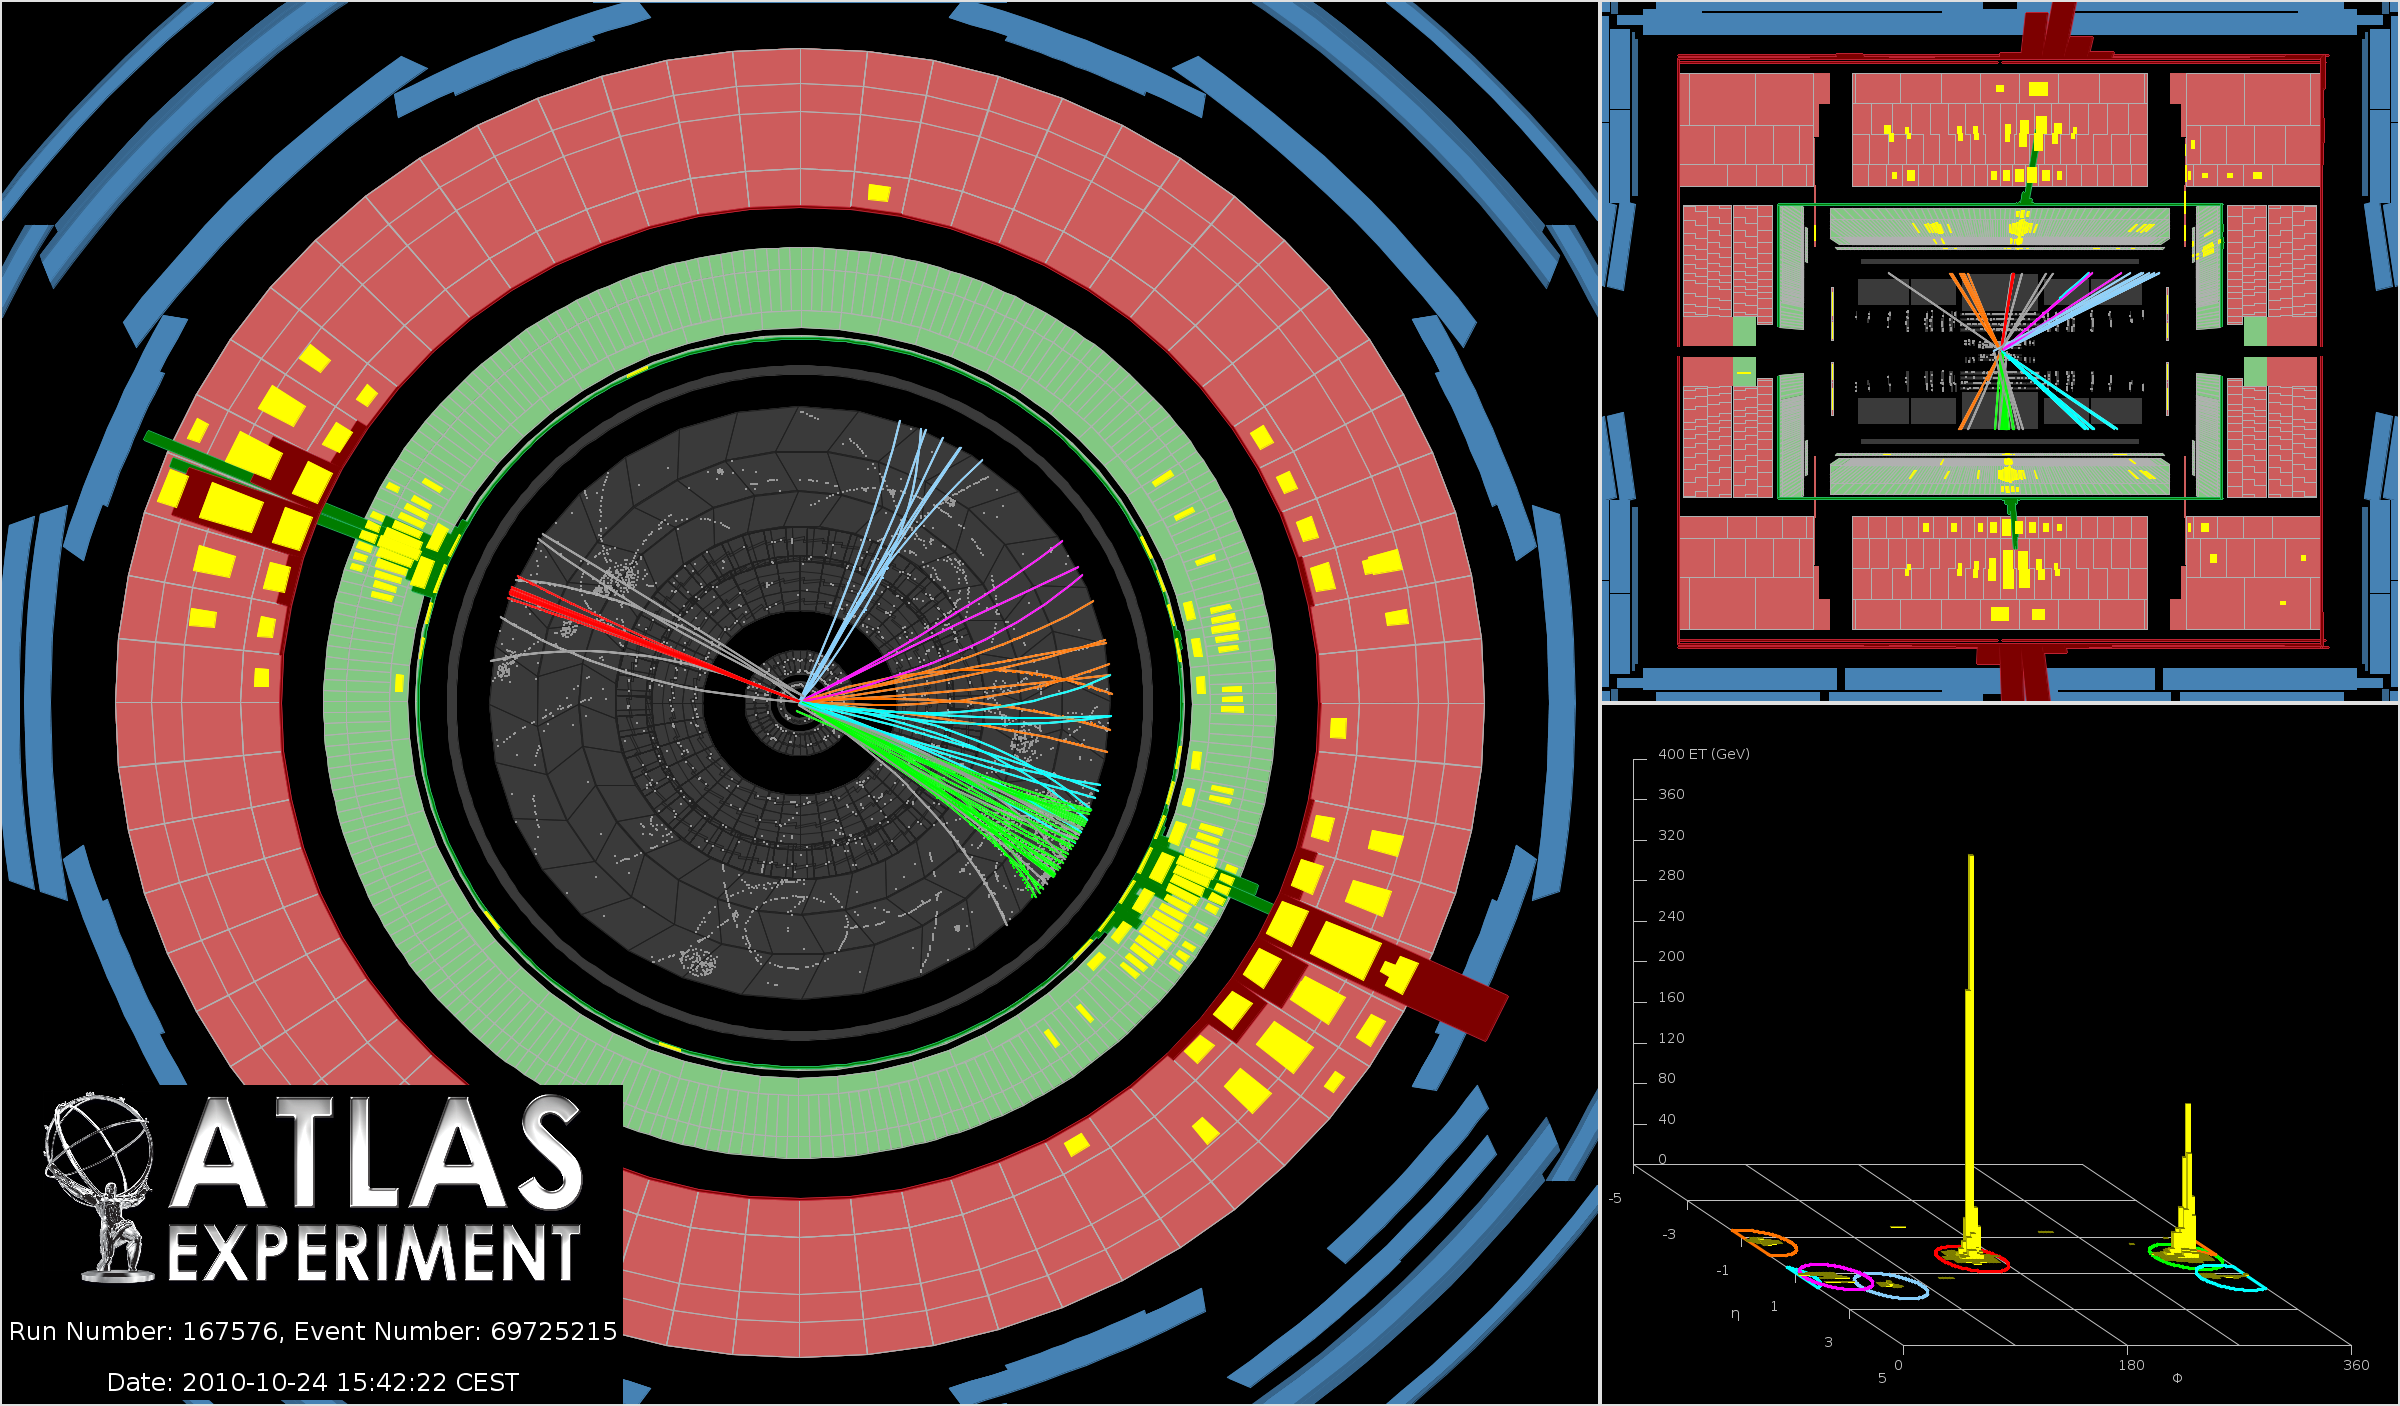
\includegraphics[width=1.\textwidth]{pics/atlasED}
}
\only<3>{
\hspace{2cm}\begin{beamercolorbox}[wd=.9\textwidth,rounded=true,shadow=true]{whiteboxcolor}\centering
{\bfseries In 2012 20.3\ifb\  collected at $\sqrt{s}=8~$TeV!}
\vspace{.3cm}

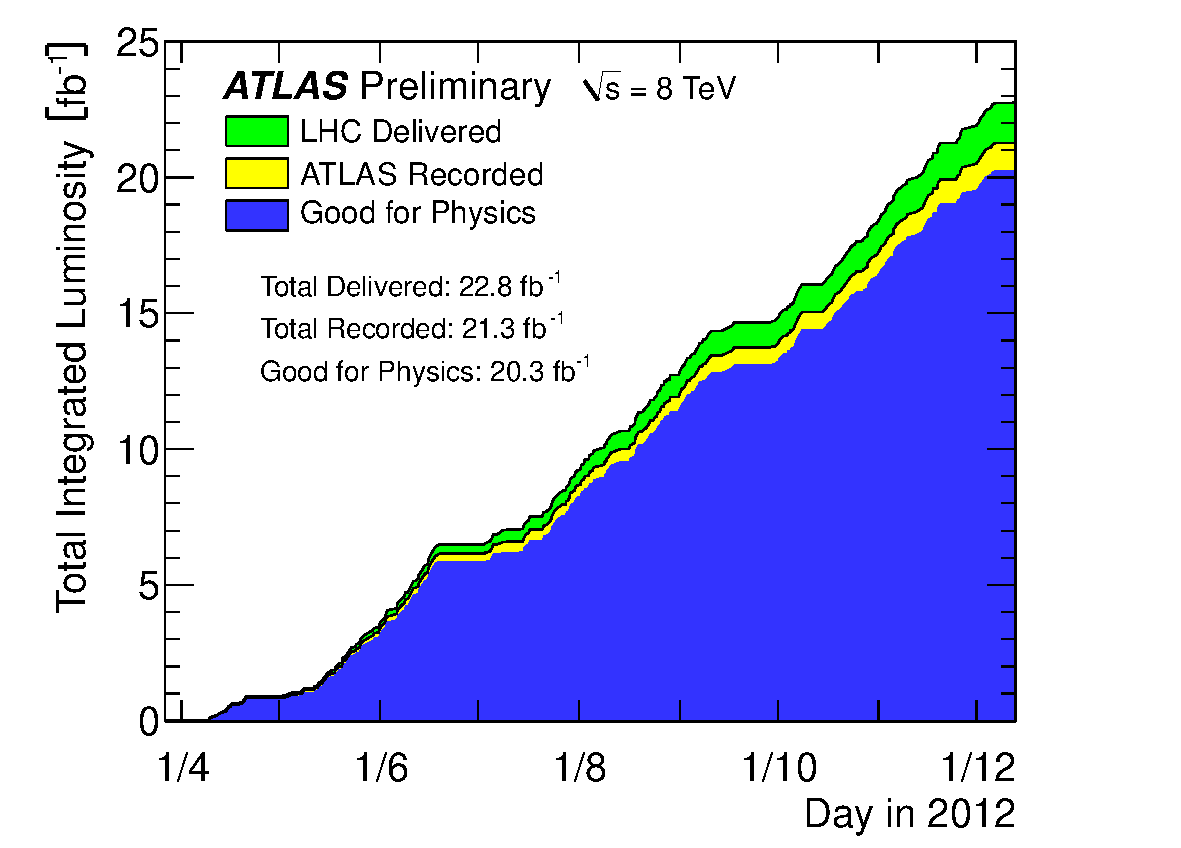
\includegraphics[width=.8\textwidth]{pics/intlumivstime2012DQ}

\vspace{\baselineskip}
%Reached peak luminosity of $3.65\times 10^{33}~$cm$^{-2}$s$^{-1}$\\
\end{beamercolorbox}
}

\end{minipage}

%Will present results obtained with \alert{14.3\ifb}\ of 2012 data

\end{frame}

\BackgroundPicture{pics/emptyIMG}

%----------------------------------
\section{Monte Carlo simulation}
%----------------------------------


%%%% EVENT1
\FullBackgroundPicture{../montecarlo/figures/event1}
\begin{frame}\frametitle{Modelling of hadron collisions}
\small\centering

\begin{flushright}\tiny Drawings from~\cite{Gieseke}\end{flushright}

want to do physics at hadron colliders?

need a good understanding of incoming hadrons

\myskip
\myskip

%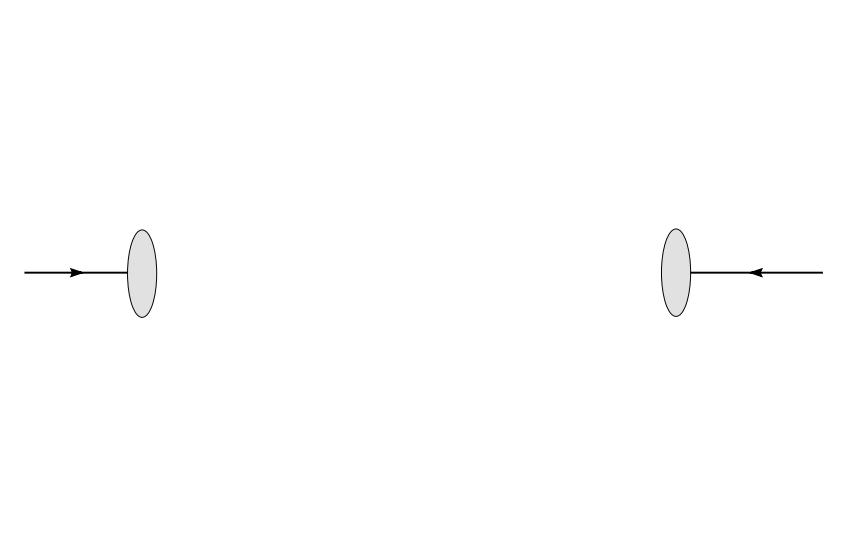
\includegraphics[height=0.8\textheight]{../montecarlo/figures/event1}

$E(p_1)=4\tev$ \hspace{.3\paperwidth} $E(p_2)=4\tev$

\vspace{.3\paperheight}

Quarks are distributed according to PDFs inside the proton\\
{\LARGE $\Downarrow$}\\
intial energy unknown, $P($valence quarks$)\sim \frac{1}{2}P(p)$

\end{frame}


%%%% EVENT1
\FullBackgroundPicture{../montecarlo/figures/event2}
\begin{frame}\frametitle{Hard scattering of two partons}
\centering\myskip
%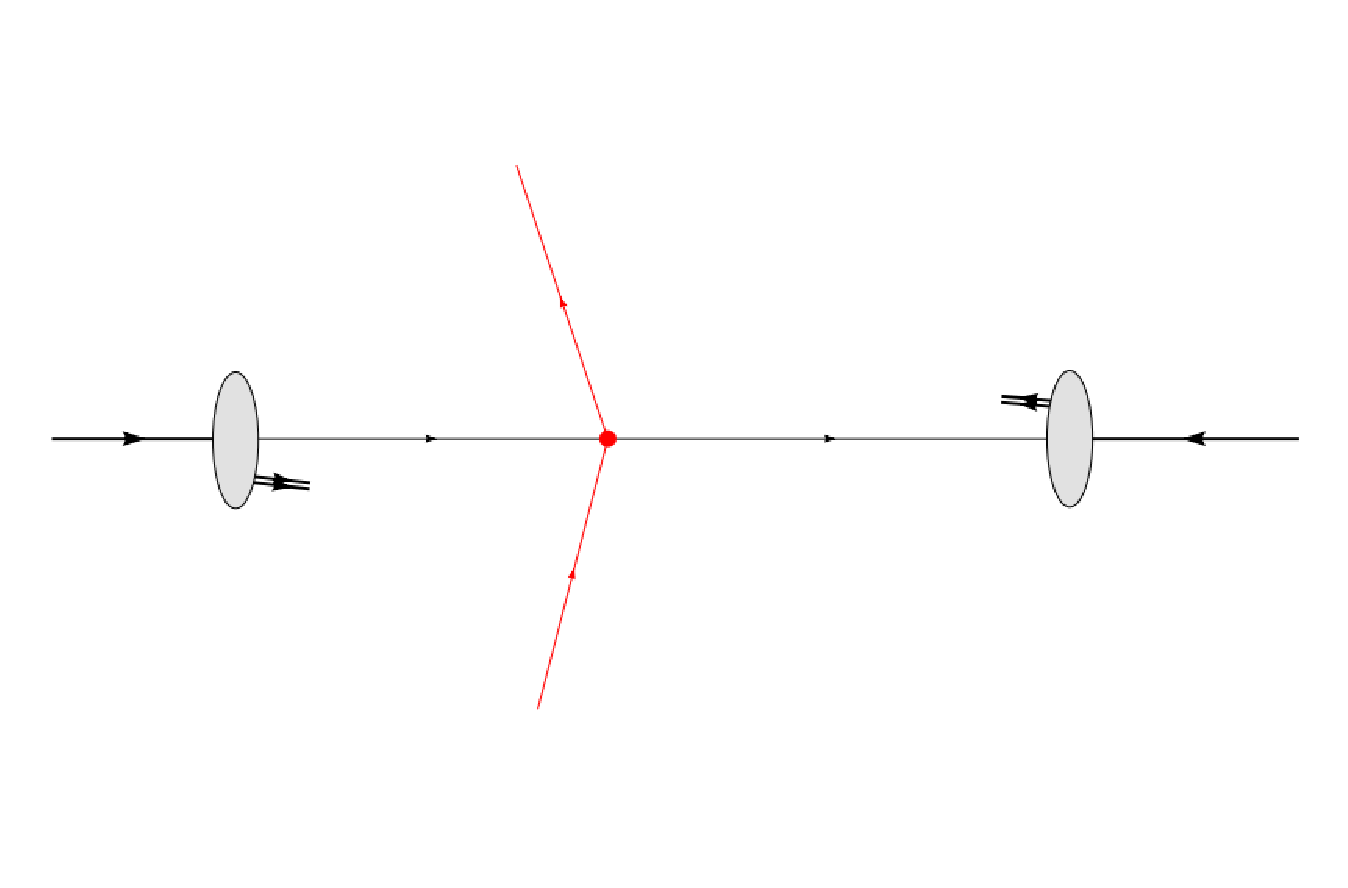
\includegraphics[height=0.8\textheight]{../montecarlo/figures/event2}

\begin{flushright}\footnotesize {\it MC: Matrix Element computation}\end{flushright}


\vspace{.5\paperheight}

{\cccolor asymptotic freedom}: high energy $\longleftrightarrow$ low \alphas\\
{\LARGE $\Downarrow$}\\
(fixed order) pQCD

\begin{flushright}\scriptsize Thanks {\cccolor factorization theorem}!
\end{flushright}

\end{frame}

%%%% EVENT1
\FullBackgroundPicture{../montecarlo/figures/event4}
\begin{frame}\frametitle{Parton showering}
\centering\myskip

\begin{flushright}\footnotesize {\it MC: iterative evolution different for\\Final- and Initial-state radiation}\end{flushright}
\begin{flushright}\footnotesize {\it ME and PS matching}\end{flushright}

\vspace{.4\paperheight}

%real radiative corrections to any inclusive quantity

QCD emission: $q\to gq$, $g\to gg$, $g\to q\bar{q}$\\
{\LARGE $\Downarrow$}\\
higher-order corrections 


\end{frame}

%%%% EVENT1
\FullBackgroundPicture{../montecarlo/figures/event6}
\begin{frame}\frametitle{Hadronization}
\centering

\begin{flushright}
\vskip-5ex

\footnotesize {\it MC: phenomenological models}\\
\includegraphics[width=.4\textwidth,height=.35\textheight]{pics/hadronization.jpg}\\
{\scriptsize\it color connections,\\ Lund string and cluster models}
\end{flushright}


\vspace{.25\paperheight}

{\cccolor confinement} @ $Q\sim 1\gev$\\
{\LARGE $\Downarrow$}\\
free partons cannot exist


\end{frame}


%%%% EVENT1
%\FullBackgroundPicture{../montecarlo/figures/event7}
\FullBackgroundPicture{../montecarlo/figures/my_collision}
\begin{frame}\frametitle{Underlying event simulation}
\centering
%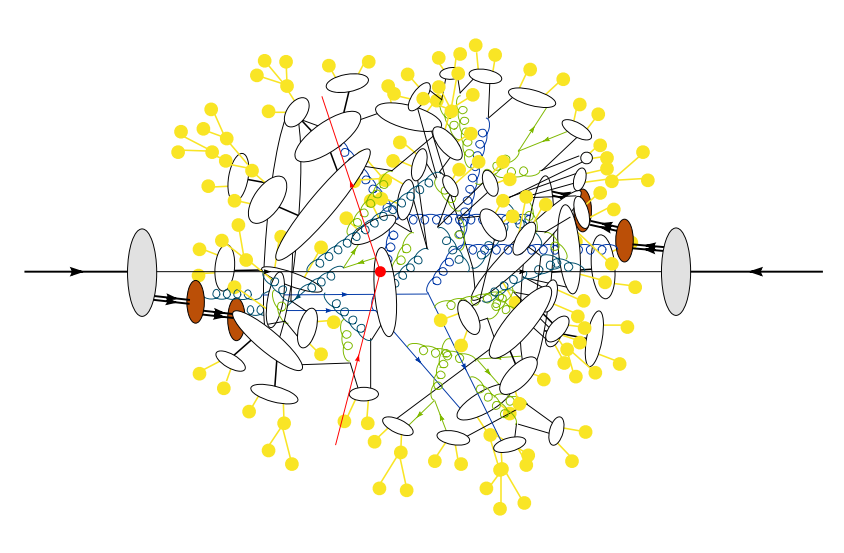
\includegraphics[height=0.8\textheight]{../montecarlo/figures/event7}


\begin{minipage}{.65\textwidth}\centering
$\quad$
\end{minipage}\begin{minipage}{.35\textwidth}\centering\myskip
hadron remnants\\ interact too\\
{\LARGE $\Downarrow$}\\
phenomenological\\ models tuned on\\
``low-\pt'' events
\end{minipage}

\vspace{.5\paperheight}


\end{frame}


\BackgroundPicture{pics/emptyIMG}
\begin{frame}\frametitle{Pile-up}
\centering\myskip

\begin{minipage}{.35\textwidth}\centering
\footnotesize

But \sout{problems} collisions\\
never come alone\dots

\begin{itemize}
\item {\cccolor in-time} and {\cccolor out-of-time} pile-up events
\end{itemize}

\myskip
high $\mathcal{L}$\\
{\LARGE $\Downarrow$}\\

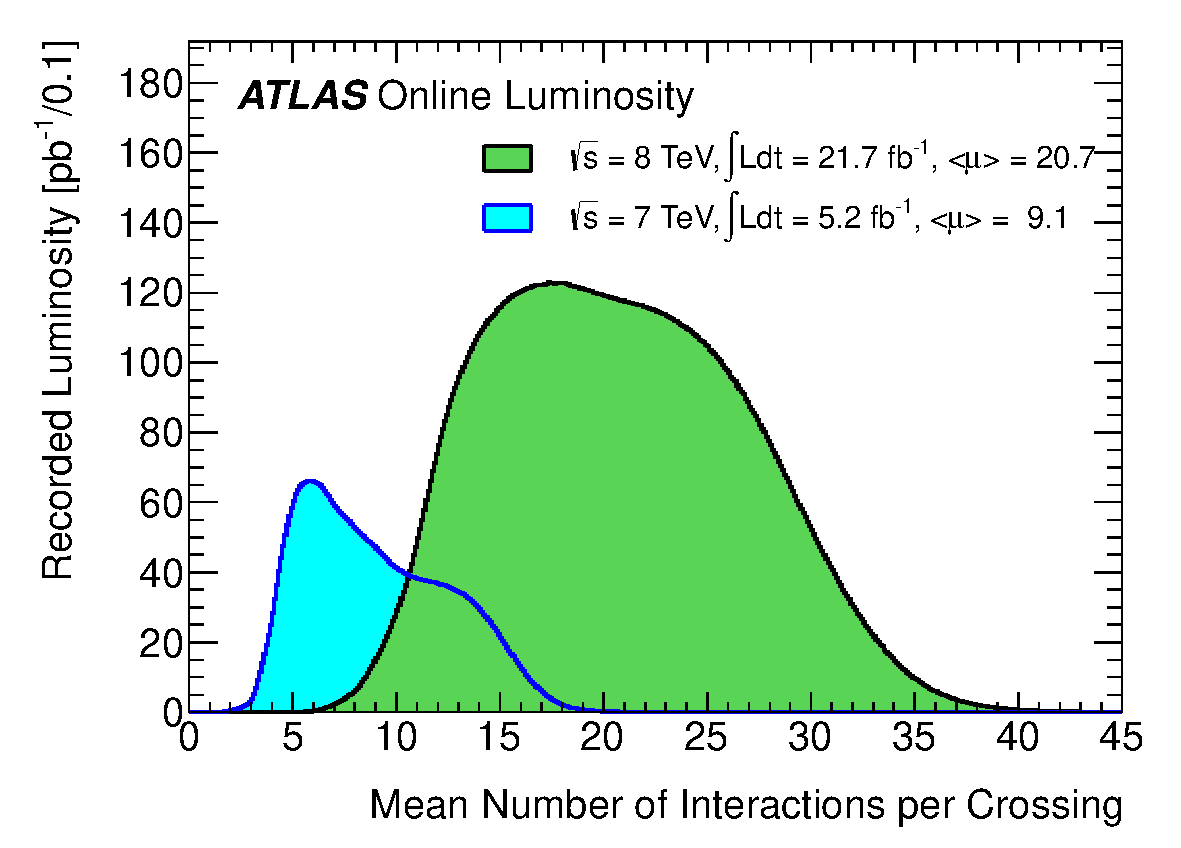
\includegraphics[width=1.\textwidth]{pics/mu_2011_2012-dec.pdf}



\end{minipage}\begin{minipage}{.65\textwidth}\centering

\vskip-5ex
\footnotesize
real $Z\to\mu\mu$ event with high pile-up (25 vertices)

\includegraphics[height=0.9\textheight,width=1.\textwidth]{pics/2012_highPileup.png}

\tiny
from \url{https://twiki.cern.ch/twiki/bin/view/AtlasPublic/EventDisplayStandAlone}
\end{minipage}

\end{frame}

\BackgroundPicture{pics/emptyIMG}

%----------------------------------
\section{Event reconstruction}
%----------------------------------

\begin{frame}\frametitle{Physics objects puzzle}
\centering\myskip

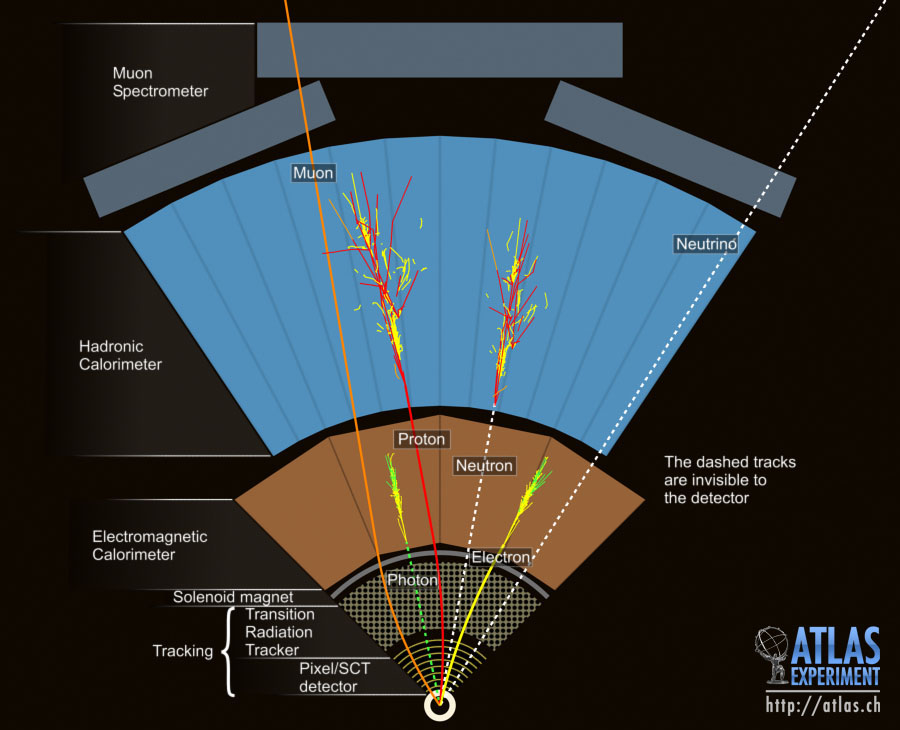
\includegraphics[height=0.85\textheight, width=1.\textwidth]{../detector/figures/detection}

\end{frame}



\begin{frame}\frametitle{One lepton}
\footnotesize\centering

\begin{minipage}{.5\textwidth}\centering
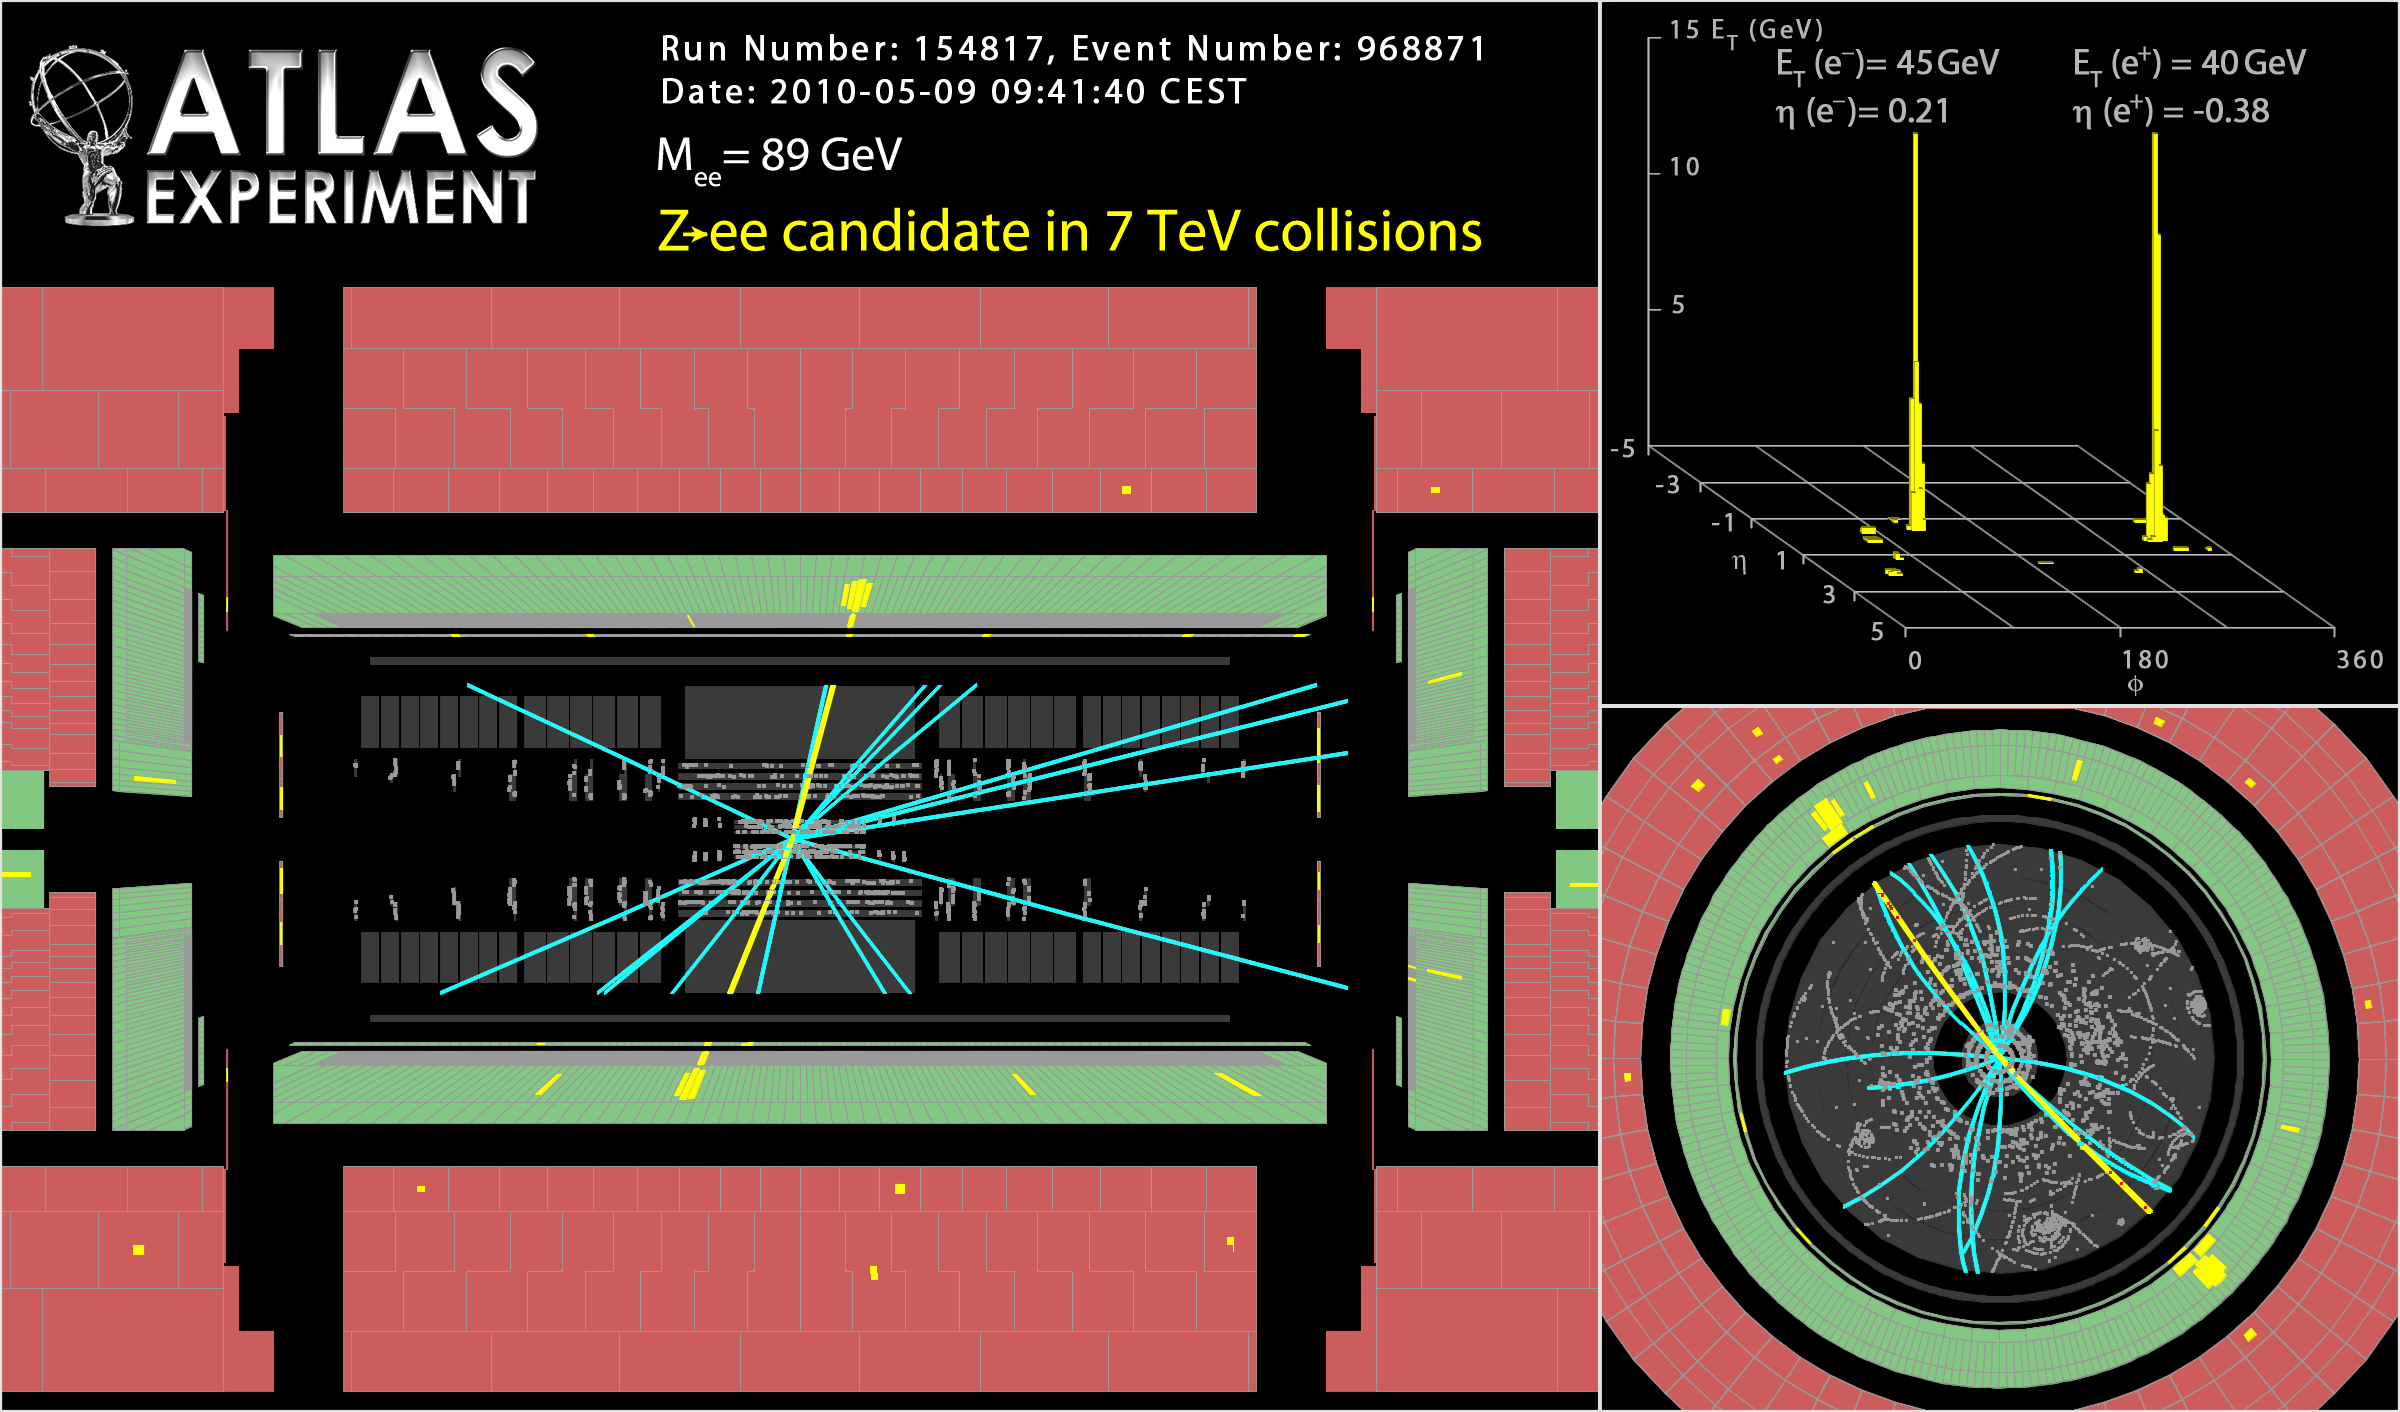
\includegraphics[width=.9\textwidth,height=0.3\textheight]{pics/Zee}

\begin{itemize}
\item $|\eta|<2.47$ ID track $\leftrightarrow$ EM deposit
\item $E_{\rm calo}$ consistent with $p_{\rm T, ID}$
\item calibrated with $Z\to ee$ events
\end{itemize}
{\cccolor \bfseries +}\\
\begin{itemize}
\item excluded $1.37< |\eta|< 1.52$
%\item $\et = E_{\rm cluster}/\cosh\eta_{\rm track} > 25\gev$, $|z_0|<2~$mm.
\item $\et > 25\gev$, $|z_0|<2~$mm
\item isolation cuts {\scriptsize\texttt{EtCone20}, \texttt{PtCone30}}
\item electron-jet overlap removal
\item {\scriptsize\texttt{EF\_e24vhi\_medium1} $||$ \texttt{EF\_e60\_medium1}}
\end{itemize}


\end{minipage}\begin{minipage}{.5\textwidth}\centering


\begin{itemize}
\item \texttt{Muid}: MS track $\leftrightarrow$ ID track ($|\eta|<2.47$)
\item $p_{\rm T,MS}$ corrected for mip loss
\item $p_{\rm T}$ weighted average MS $\leftrightarrow$ ID
\item calibrated with $Z\to \mu\mu$ events
\end{itemize}
{\cccolor \bfseries +}\\
\begin{itemize}
\item $\pt > 25\gev$, $|z_0|<2~$mm
\item isolation cut \texttt{PtCone20}
\item mini-isolation cut
\item \texttt{EF\_mu24i\_tight} $||$ \texttt{EF\_mu36\_tight}
\end{itemize}

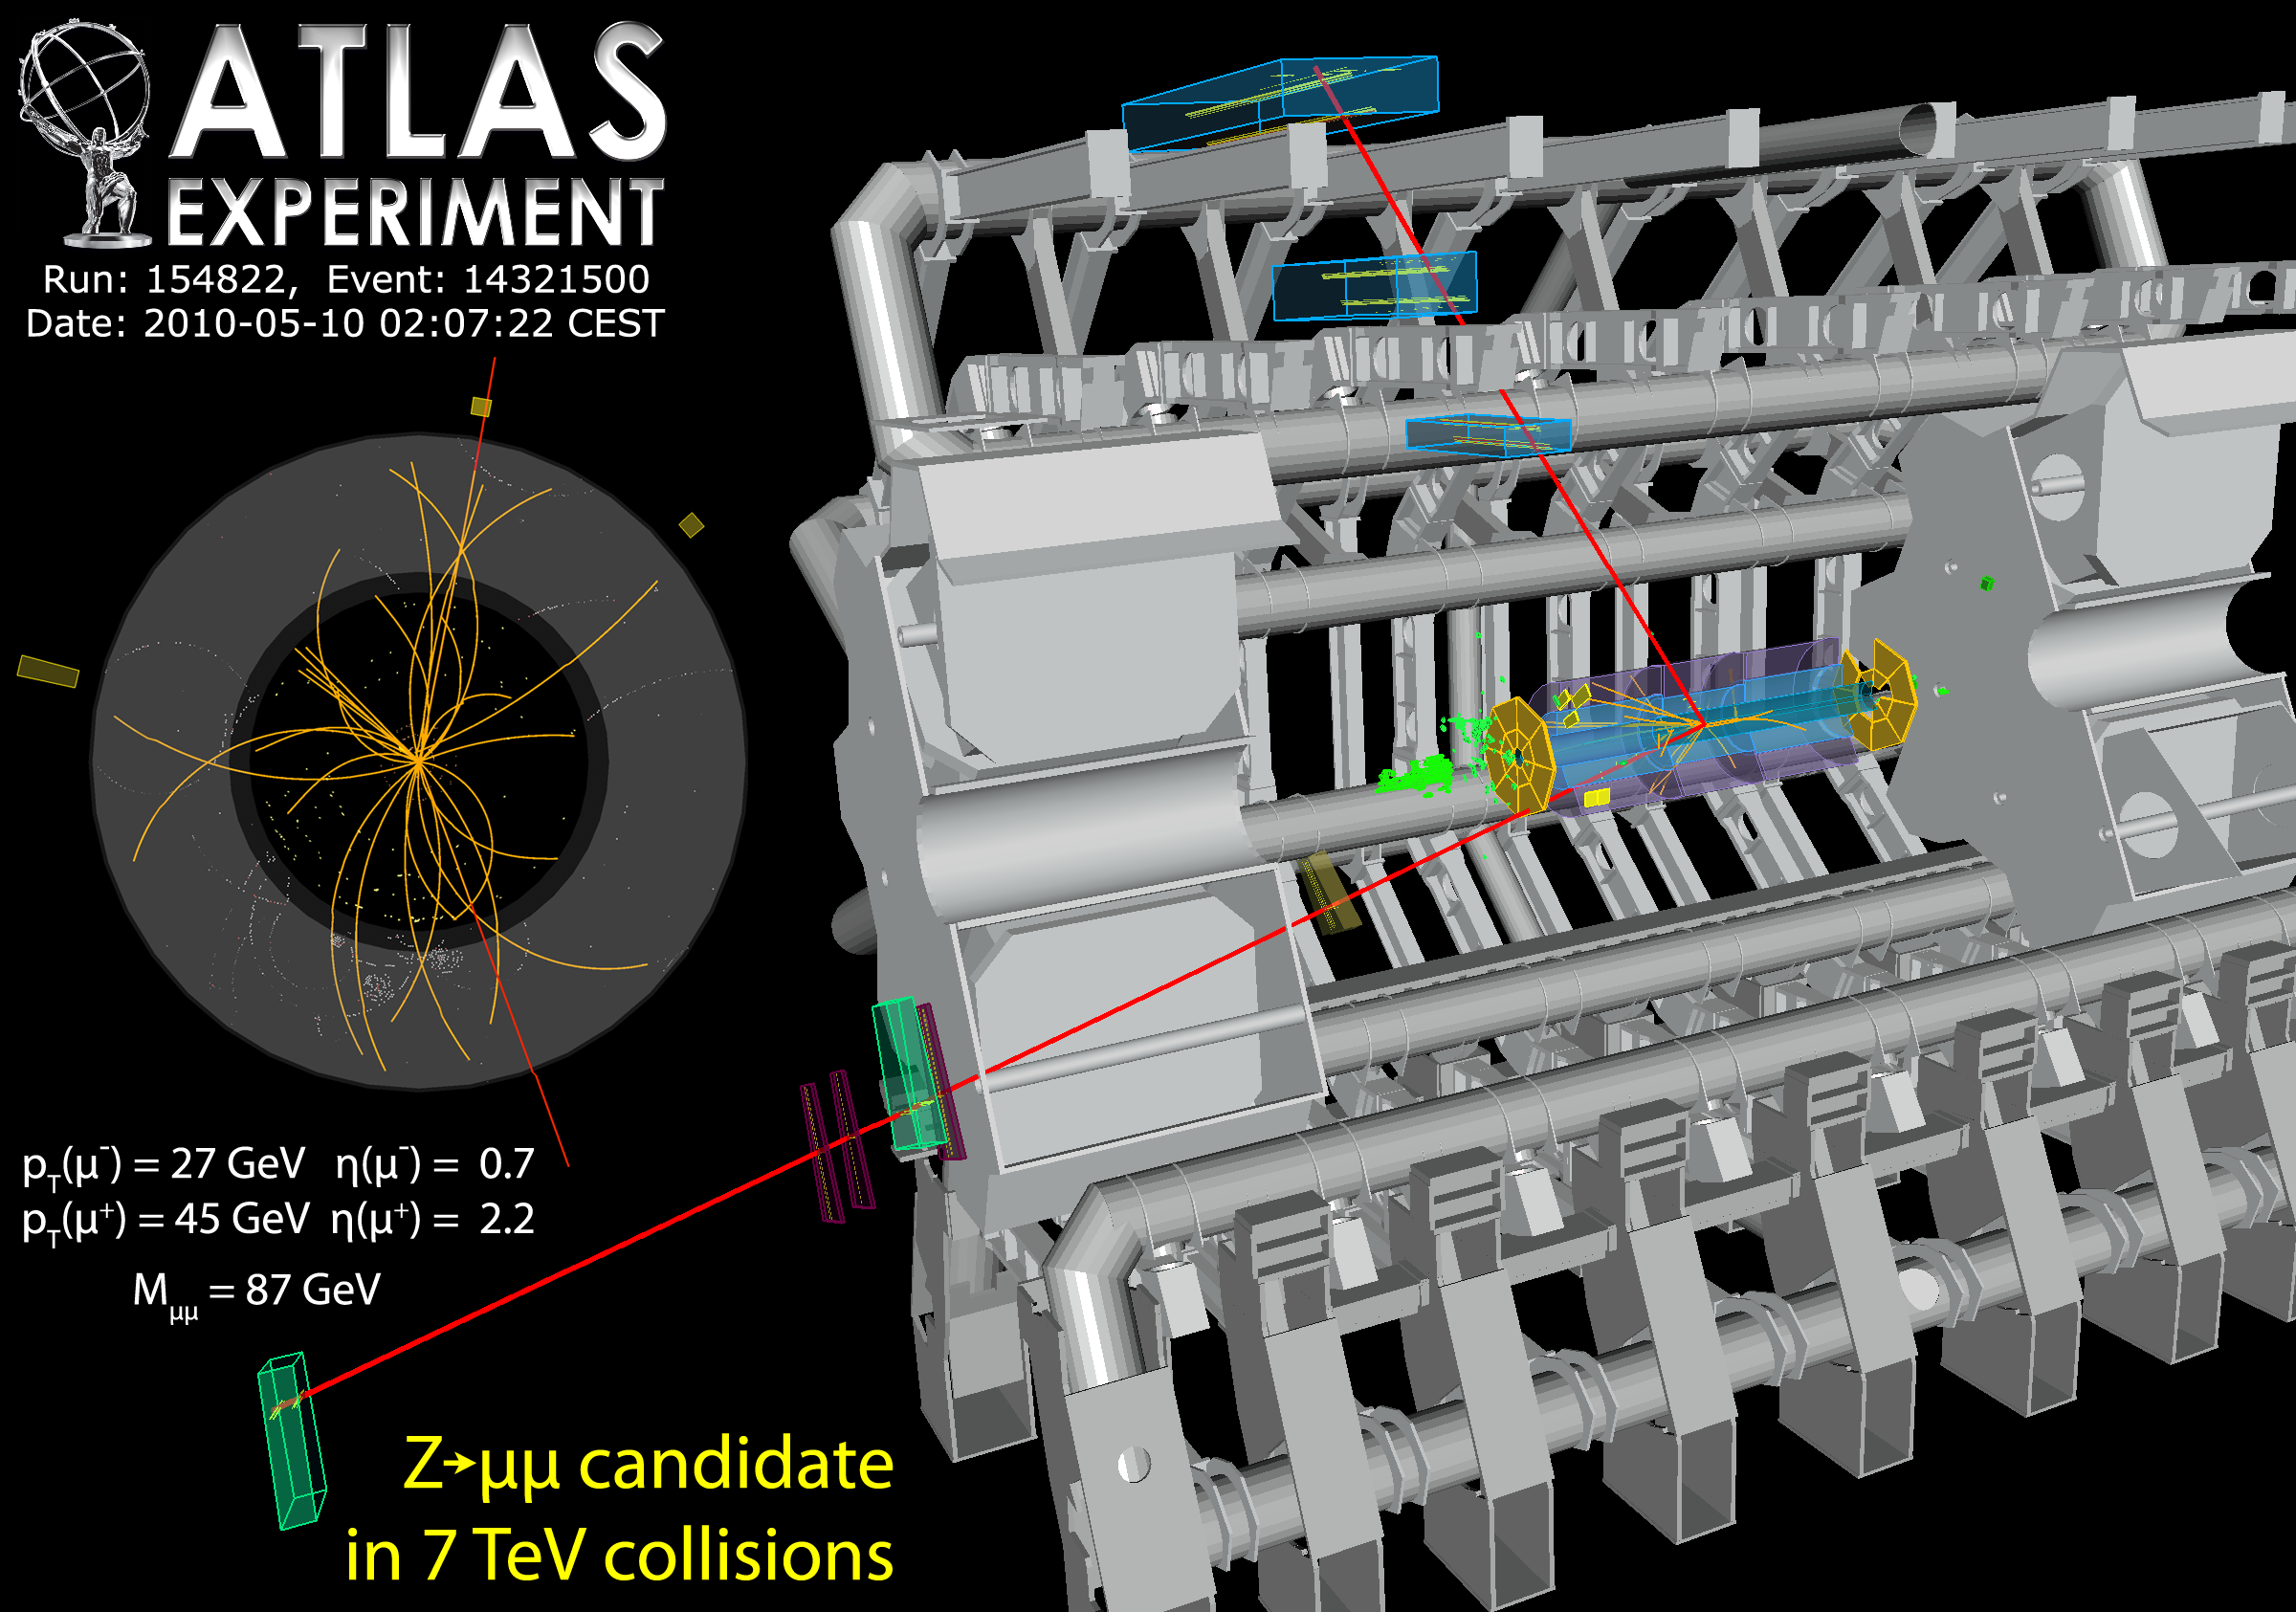
\includegraphics[width=.78\textwidth,height=0.3\textheight]{pics/Zmumu}

\end{minipage}


\end{frame}



\begin{frame}\frametitle{Many jets}
\centering\footnotesize

\begin{minipage}{.5\textwidth}\centering

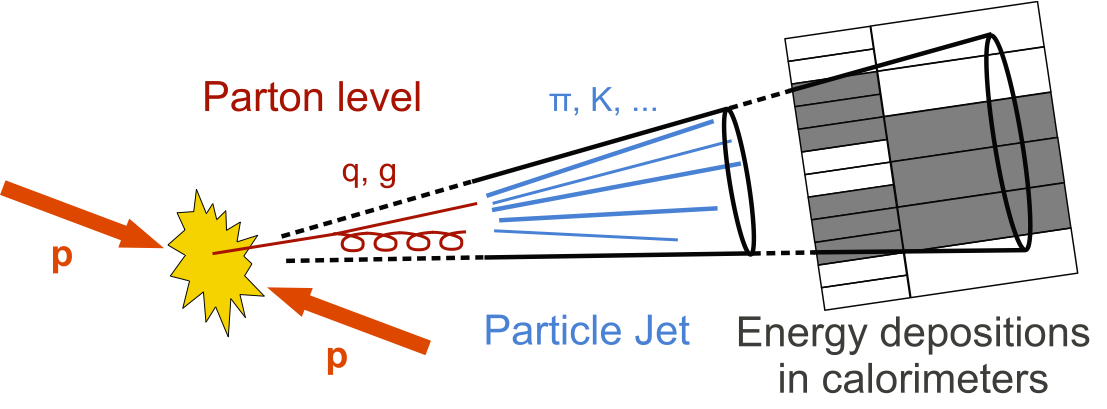
\includegraphics[width=.78\textwidth]{pics/Sketch_PartonParticleCaloJet.png}\\
%\resizebox{1.\textwidth}{!}{from \url{http://cms.web.cern.ch/news/jets-cms-and-determination-their-energy-scale}}

\begin{itemize}
\item Combine calorimeter clusters using anti-$k_t$ algorithm with $R=0.4$
\end{itemize}
$d_{ij}=min(\dfrac{1}{k_{t_i}^{2}},\dfrac{1}{k_{t_j}^{2}})\frac{\Delta R_{ij}^{2}}{R^{2}}$
\begin{itemize}
\item LC clusters energy
\item Pile-up and JES correction
\end{itemize}
{\cccolor \bfseries +}\\
\begin{itemize}
\item $\pt>25\gev$, $|\eta|<2.5$
\item JVF$>0.5$
\item jet-electron overlap removal
\end{itemize}


\end{minipage}\begin{minipage}{.5\textwidth}\centering
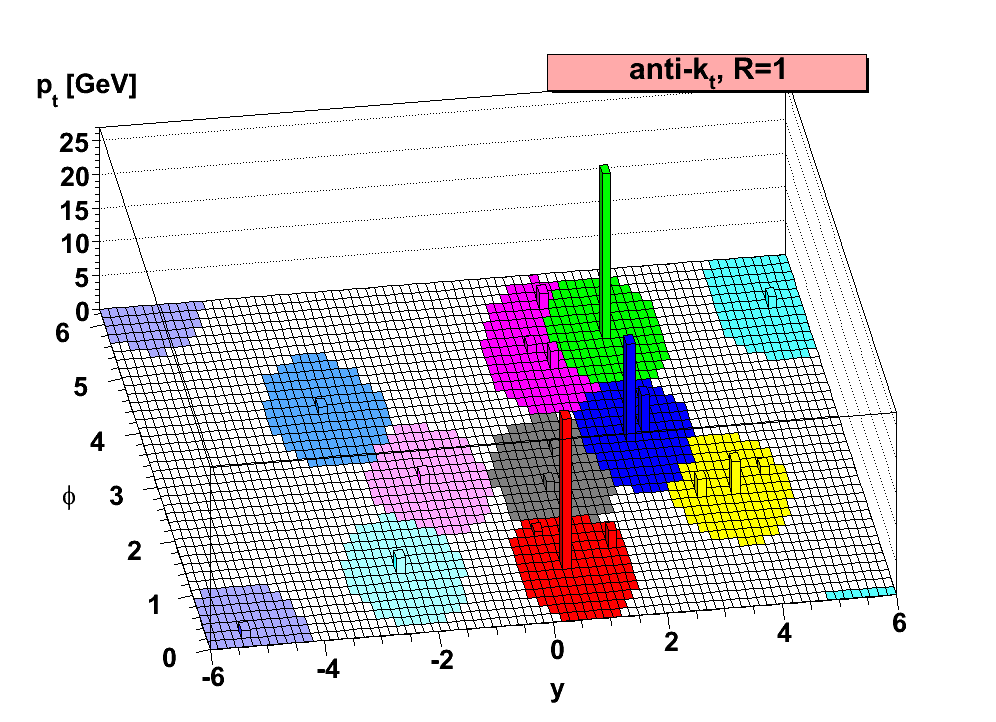
\includegraphics[width=.78\textwidth]{pics/antikt}\\
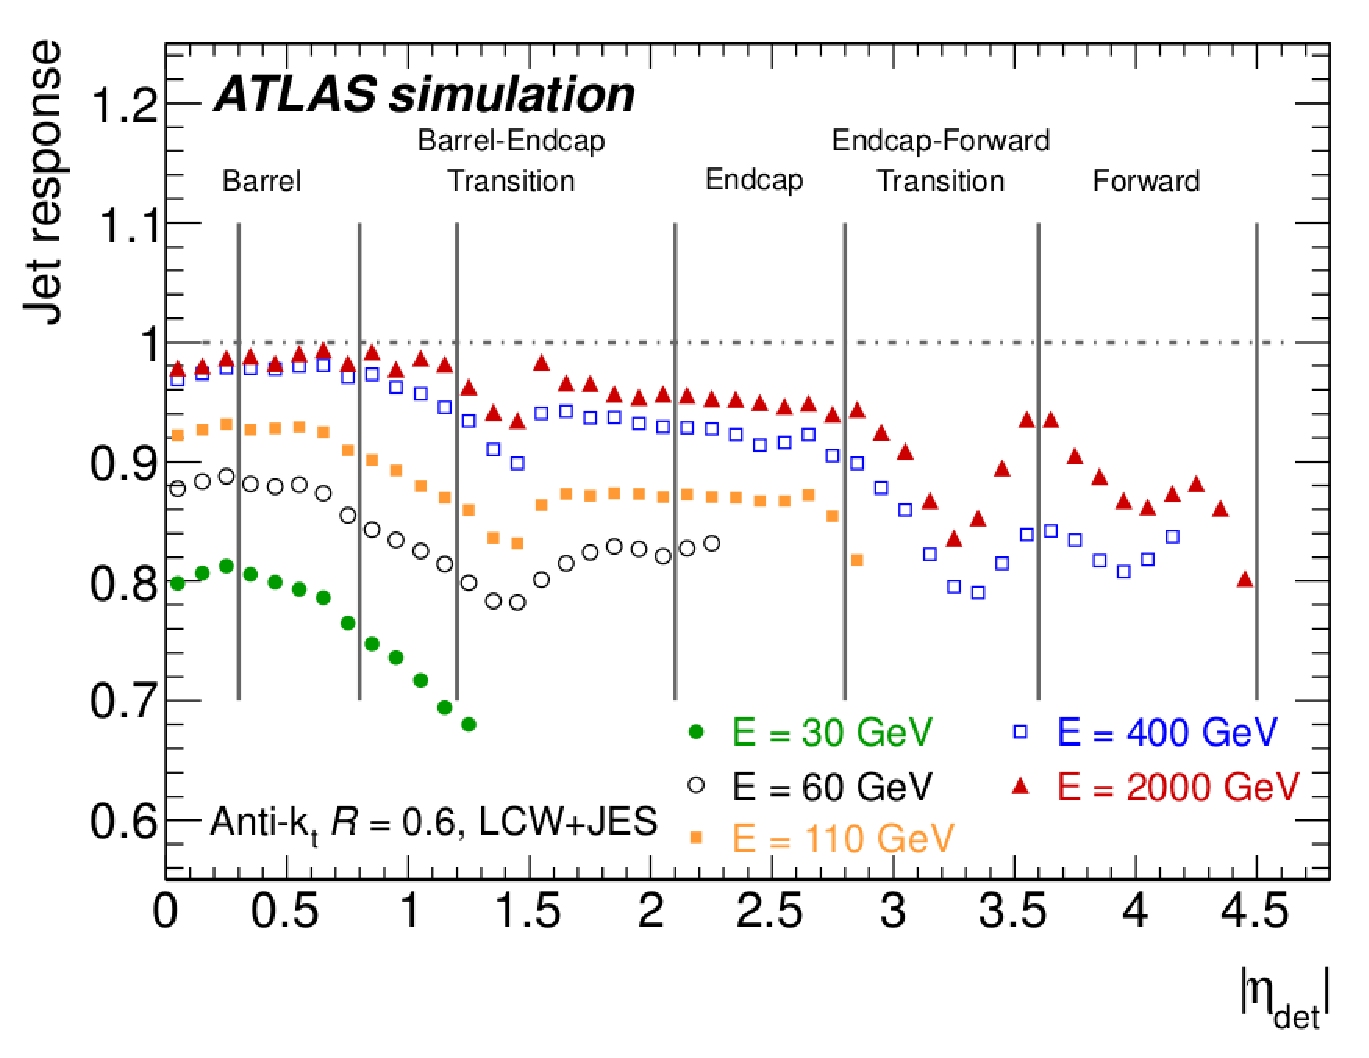
\includegraphics[width=.9\textwidth]{pics/corr_jet_lcw}

\end{minipage}


\end{frame}



\begin{frame}\frametitle{\btag ging}
\centering\footnotesize

\begin{minipage}{.3\textwidth}\centering

$b$ quark $\Rightarrow$ $B$ hadron ($\lambda\sim 10^{-12}$~s)\\
{\large$\Downarrow$}\\
travels about 3~mm\\ before decaying

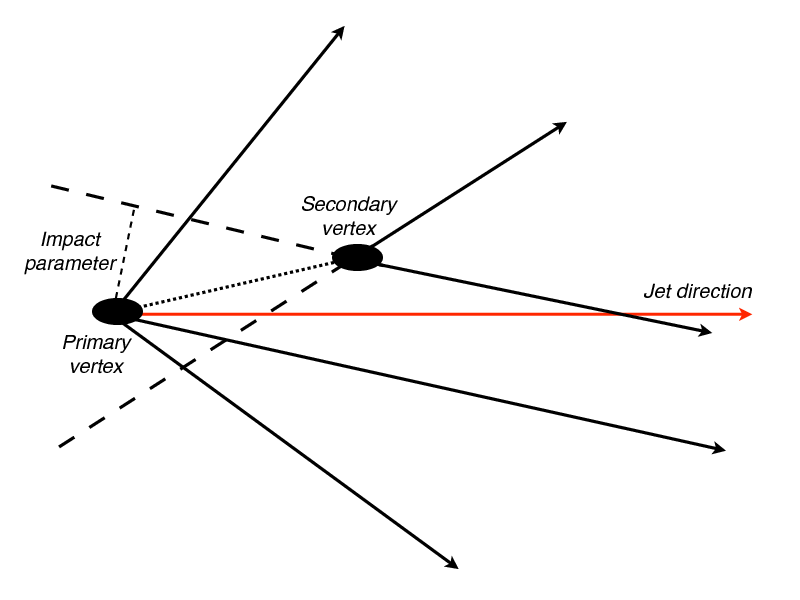
\includegraphics[width=.8\textwidth]{../objectsreconstruction/figures/Picture-b-tagging-2.png}

\end{minipage}\begin{minipage}{.7\textwidth}\centering

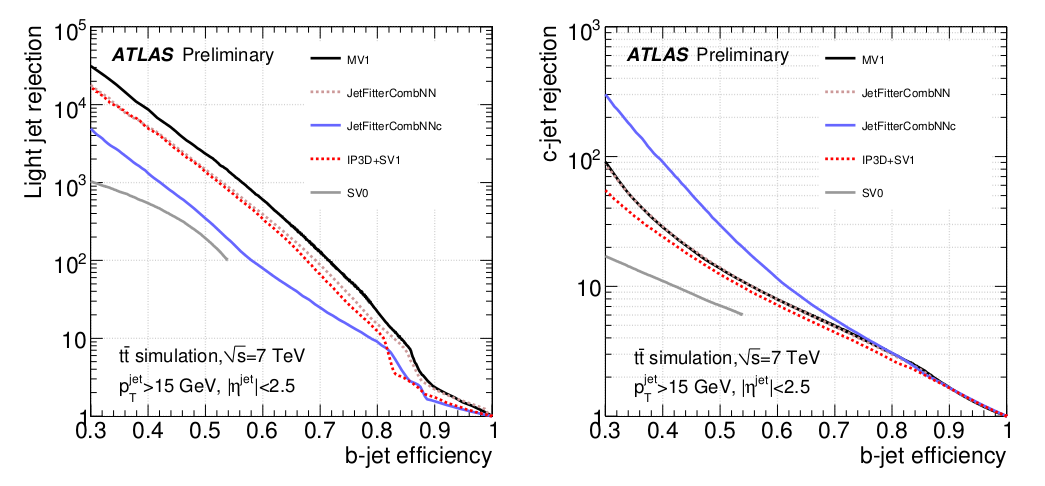
\includegraphics[width=1.\textwidth]{../objectsreconstruction/figures/btageffs.png}

\end{minipage}

\myskip

\begin{minipage}{.4\textwidth}\centering


various algorithms exploit ID track info to identify \bjet s

\begin{itemize}
\item \texttt{\cccolor MV1} algorithm @ 70\% efficiency, $\sim 130$ rejection
\end{itemize}

\end{minipage}\begin{minipage}{.6\textwidth}\centering

Events are selected through \\a cut on the \btag-weight computed\\
{\large$\Downarrow$}\\
with 70\% efficiency, high multiplicities will suffer

\begin{itemize}
\item {\cccolor TagRateFunction} method
\end{itemize}


\end{minipage}


\end{frame}



\begin{frame}\frametitle{Missing transverse energy}
\centering\myskip

\begin{minipage}{.5\textwidth}\centering

\includegraphics[width=.9\textwidth]{pics/real_et}\\
{\tiny from \url{http://tomwhyntie.wordpress.com/research/}}

\end{minipage}\begin{minipage}{.5\textwidth}\centering
\end{minipage}
$$\begin{array}{lcl}
%E^{\rm miss}_{x,y} & = & E^{\rm RefEle}_{x,y} + E^{\rm RefGamma}_{x,y} + E^{\rm RefJet}_{x,y} + E^{\rm RefMuon}_{x,y} + E^{\rm SoftJet}_{x,y} + E^{\rm CellOut}_{x,y}\\
E^{\rm miss}_{T} & = & \big|-\sum\vec{p}_T \big| = \sqrt{(E^{\rm miss}_{x})^2 + (E^{\rm miss}_{y})^2} ,\\
E^{\rm miss}_{x} & = & -\sum\vec{p}_x ,\\
E^{\rm miss}_{y} & = & -\sum\vec{p}_y ,\\
\end{array}$$


\end{frame}



%----------------------------------
\section{Searches for \TTbar\ in single lepton channel}
%----------------------------------
\begin{frame}\frametitle{Allowed decay modes}
\centering\myskip

\begin{minipage}{.4\textwidth}\centering
\scriptsize
  \begin{tabular}{cc}\toprule
Singlet & Decay modes\\ 
& \\
$T(+2/3)$ & $\alert{ W^+b},\, \alert{ Ht},\, Zt$ \\
& \\
$B(-1/3)$ & $ W^-t,\, Hb,\, Zb$ \\
& \\
$X(+5/3)$ & $W^+t$\\
& \\
$Y(-4/3)$ & \alert{$W^-b$} \\
& \\\midrule
Doublet & Decay modes\\
 &\\
 \multirow{2}{*}{$\bigg(\begin{array}{c}T \\ B\end{array}\bigg)$} & $\alert{ W^+b},\, \alert{ Ht},\, Zt$ \\
 & $ W^-t,\, Hb,\, Zb$\\
 & \\
\multirow{2}{*}{$\bigg(\begin{array}{c}T \\ X\end{array}\bigg)$} & $\alert{ Ht},\, Zt$\\
 & $W^+t$\\
 &\\
 \multirow{2}{*}{$\bigg(\begin{array}{c}B \\ Y\end{array}\bigg)$} & $Hb,\, Zb$\\
 & \alert{$W^-b$}\\
\bottomrule
\end{tabular}

\end{minipage}\begin{minipage}{.6\textwidth}\centering
  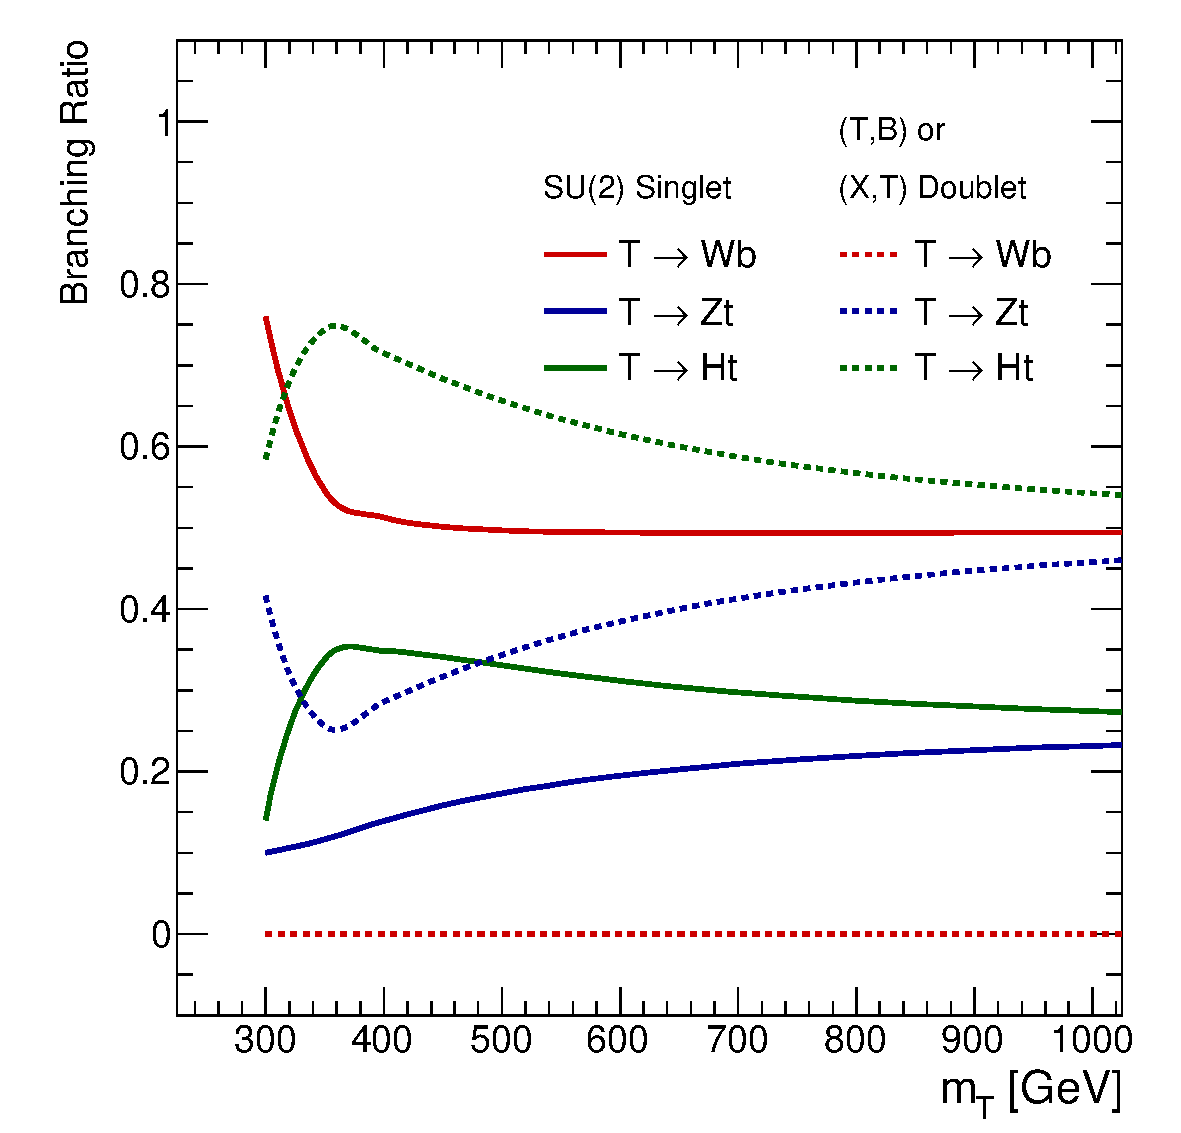
\includegraphics[width=0.95\textwidth]{../vlq_analysis/figures/fig_02a.pdf}
\end{minipage}

\end{frame}




\begin{frame}\frametitle{Model Independent Strategy}
\footnotesize\centering


\begin{pgfpicture}{0.0\textwidth}{0.0\textheight}{1.\textwidth}{.6\textwidth}

\begin{pgfscope}
\pgfdeclareimage[interpolate=true,width=.45\textwidth]{tab}{pics/tabBRs}
\onslide<1->{
    \pgfsetendarrow{\pgfarrowlargepointed{6pt}}
    \pgfsetlinewidth{1.5pt}
    \usebeamercolor[fg]{head/foot boxes}
    \begin{pgftranslate}{\pgfpoint{0.07\textwidth}{0.15\textheight}}
\pgfline{\pgfxy(0,0)}{\pgfxy(5.5,0)}
\pgfstroke
\pgfputat{\pgfxy(3.5,-0.5)}{\pgfbox[left,base]{BR($T\to Wb$)}}
    \usebeamercolor[fg]{normal text}
\pgfcircle[fill]{\pgfxy(6.8,4.1)}{2pt}
\pgfputat{\pgfxy(7,4)}{\pgfbox[left,base]{Build a 2-dim plane}}
\pgfputat{\pgfxy(7,3.7)}{\pgfbox[left,base]{to scan model mixing}}
%    \end{pgftranslate}
%\end{pgfscope}
}
%\pause
\onslide<2->{
%\begin{pgfscope}
    \pgfsetendarrow{\pgfarrowlargepointed{6pt}}
    \pgfsetlinewidth{1.5pt}
    \usebeamercolor[fg]{head/foot boxes}
%    \begin{pgftranslate}{\pgfpoint{0.1\textwidth}{0.15\textheight}}
    \usebeamercolor[fg]{head/foot boxes}
\pgfline{\pgfxy(0,0)}{\pgfxy(0,5.5)}
\pgfstroke
    \begin{pgfrotateby}{\pgfdegree{90}}
\pgfputat{\pgfxy(3.5,0.4)}{\pgfbox[left,base]{BR($T\to Ht$)}}
    \end{pgfrotateby}
%    \end{pgftranslate}
%\end{pgfscope}
}
\onslide<3->{
    \usebeamercolor[bg]{head/foot boxes}
    \pgfcircle[fill]{\pgfxy(5.,0)}{3pt}
    \pgfcircle[fill]{\pgfxy(2.5,1.5)}{3pt}
    \pgfcircle[fill]{\pgfxy(0.,3.)}{3pt}
    \pgfputat{\pgfxy(5.5,4.7)}{\pgfbox[left,base]{\pgfuseimage{tab}}}
}
%\pause
\onslide<4->{
%\begin{pgfscope}
    \pgfsetlinewidth{1.5pt}
    \color{light-gray}
%    \begin{pgftranslate}{\pgfpoint{0.1\textwidth}{0.15\textheight}}
%\pgfline{\pgfxy(5,0)}{\pgfxy(0,5)}
%\pgfstroke
\pgfmoveto{\pgfxy(5,0)}
\pgflineto{\pgfxy(5,5)}
\pgflineto{\pgfxy(0,5)}
%\pgfstroke
\pgffill
    \color{gray}
\pgfputlabelrotated{0.5}{\pgfxy(0,5)}{\pgfxy(5,0)}{8pt}{\pgfbox[center,base]{Forbidden}}
    \usebeamercolor[fg]{normal text}
\pgfcircle[fill]{\pgfxy(6.8,3.3)}{2pt}
\pgfputat{\pgfxy(7,3.2)}{\pgfbox[left,base]{Sum of BRs is 1$^{(a)}$}}
%\pgfputat{\pgfxy(5.2,0.7)}{\pgfbox[left,base]{\scriptsize $^{(a)}$BR($T\to  Zt/b$) = 1 - BR($T\to Ht/b$) - BR($T\to Wb/t$)}}
\pgfputat{\pgfxy(5.9,-0.9)}{\pgfbox[left,base]{\scriptsize $^{(a)}$BR($T\to  Zt$) = 1 - BR($T\to Ht$) - BR($T\to Wb$)}}
%\pgfputat{\pgfxy(8.755,-0.7)}{\pgfbox[left,base]{\scriptsize - BR($T\to Wb$)}}
{
    \usebeamercolor[bg]{head/foot boxes}
    \pgfcircle[fill]{\pgfxy(5.,0)}{3pt}
}
%    \end{pgftranslate}
%\end{pgfscope}
}
%\pause
\onslide<5->{
%\begin{pgfscope}
    \pgfsetlinewidth{1.5pt}
%    \begin{pgftranslate}{\pgfpoint{0.1\textwidth}{0.15\textheight}}
    \usebeamercolor[fg]{normal text}
\pgfcircle[fill]{\pgfxy(6.8,2.8)}{2pt}
\pgfputat{\pgfxy(7,2.7)}{\pgfbox[left,base]{Different analyses are}}
\pgfputat{\pgfxy(7,2.4)}{\pgfbox[left,base]{sensitive to different areas}}
    \usebeamercolor[fg]{head/foot boxes}
\begin{pgfscope}
\pgfmoveto{\pgfxy(5,0)}
\pgflineto{\pgfxy(0,0)}
\pgflineto{\pgfxy(0,5)}
\pgfclip
\pgfcircle[fill]{\pgfxy(.5,4)}{55pt}
{\usebeamercolor[bg]{normal text}
%\pgfputat{\pgfxy(0.,3.5)}{\begin{pgfrotateby}{\pgfdegree{-45}}\pgfbox[left,base]{$T(B)\to Ht(b)$}\end{pgfrotateby}}
\pgfputat{\pgfxy(0.05,3.2)}{\pgfbox[left,base]{\large$Ht+X$}}
}
{
    \usebeamercolor[bg]{head/foot boxes}
    \pgfcircle[fill]{\pgfxy(0.,3.)}{3pt}
}
}
\pgfcircle[fill]{\pgfxy(4,0)}{35pt}
{\usebeamercolor[bg]{normal text}
%\pgfputat{\pgfxy(3.,0.4)}{\pgfbox[left,base]{$T(B)\to Wb(t)$}}
\pgfputat{\pgfxy(2.9,0.2)}{\pgfbox[left,base]{\large$Wb+X$}}
}
{
    \usebeamercolor[bg]{head/foot boxes}
    \pgfcircle[fill]{\pgfxy(5.,0)}{3pt}
}
\end{pgfscope}
\onslide<6->{
\usebeamercolor[fg]{normal text}
%\pgfcircle[fill]{\pgfxy(6.8,2.)}{2pt}
%\pgfputat{\pgfxy(7,1.9)}{\pgfbox[left,base]{Set exclusion using $CL_{s}$ }}
%\pgfputat{\pgfxy(7,1.6)}{\pgfbox[left,base]{in each point of the plane}}
%\pgfcircle[fill]{\pgfxy(6.8,1.2)}{2pt}
\pgfputat{\pgfxy(5.3,1.)}{\pgfbox[left,base]{\begin{tabular}{c c c} 
Set strategy & \multirow{2}{*}{$\Rightarrow$} & Check good bkg \\
($S/B$)      &                                & modeling \\
             &                                &  $\Downarrow$\\
Test \cls{b} and & \multirow{2}{*}{$\Leftarrow$} & \multirow{2}{*}{Look at data} \\
\cls{s+b} hypotheses & &\\
\multicolumn{3}{c}{$\nwarrow$} \\
\multicolumn{3}{c}{\it for each point of the BR plane}\\
\end{tabular}}}
}
    \end{pgftranslate}
\end{pgfscope}
\end{pgfpicture}

\end{frame}





\begin{frame}\frametitle{Preselection}
\centering\myskip

\begin{minipage}{.6\textwidth}\centering\footnotesize
Two searches using common analysis framework:
\begin{minipage}{.5\textwidth}\centering
\begin{itemize}
\item \wbx
\end{itemize}
\scriptsize
\cccolor 

ATLAS-CONF-2013-060~\cite{ATLAS-CONF-2013-060}
\end{minipage}\begin{minipage}{.5\textwidth}\centering
\begin{itemize}
\item \htx
\end{itemize}
\scriptsize
\cccolor 

ATLAS-CONF-2013-018~\cite{ATLAS-CONF-2013-018}
\end{minipage}

\myskip

\begin{tabular}{ll}
\toprule
Preselection stage & Requirements \\
\midrule
Single lepton & One electron or muon\\
              & matching trigger  \\\midrule
%\\
QCD rejection & $\met >20\gev$\\
              & $\met +m_{\rm T}>60\gev$ \\\midrule
%\\
Jet multiplicity & $\geq 4$ jets\\
                 & $\geq 1$ $b$-tagged jets \\
\bottomrule\end{tabular}

\myskip
{\bfseries\cccolor orthogonality requirements:} 

\begin{itemize}
\item \wbx: reject events with $\geq$6 jets and $\quad$ $\geq$3 \bjet s
\item \htx: reject events in the low \btag s channel with $\HT<700\gev$
\end{itemize}

\myskip

\end{minipage}\begin{minipage}{.4\textwidth}\centering
\vskip-5ex
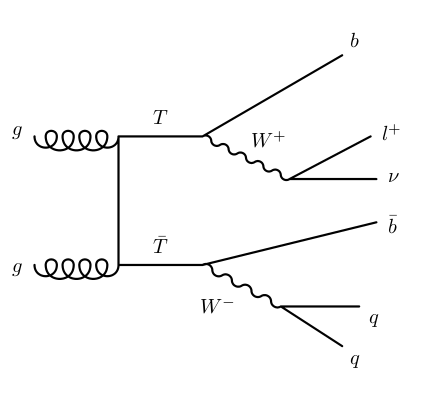
\includegraphics[width=0.9\textwidth]{pics/feyn_wbwb}\\
\vskip-2ex
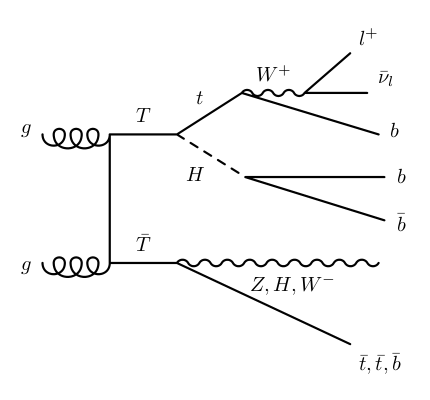
\includegraphics[width=0.9\textwidth]{pics/feyn_htX}
\end{minipage}


\end{frame}



\begin{frame}\frametitle{Background and signal modelling}
\centering\myskip

\begin{minipage}{.5\textwidth}\centering
\scriptsize
Yields in the preselection region ``blinded'' as:\\
$\htfj<800\gev$ (*)
\myskip

  \begin{tabular}{l D{;}{\,\pm\,}{-1} } \toprule
 & \multicolumn{1}{c}{ $\geq 4$ jets, $\geq 1$ $b$-tags } 		 \\ \midrule 
\rowcolor{LightCyan}  Multi-jet  & 6264;74 \\ 
 Single top  & 14375;107 \\ 
 Diboson  & 548;12 \\ 
 $Z$+jets  & 5804;146 \\ 
 $W$+jets  & 35921;525 \\ 
 $t\bar{t}$V & 680;2 \\ 
 $t\bar{t}$H (125)  & 220;1 \\ 
 $t\bar{t}$ MC@NLO  & 202042;285 \\ 
\midrule 
  Tot Bkg w/ MC@NLO  & 265854;629 \\ \midrule 
  $T\bar{T}$ (600) chiral  & 36;2 \\ 
 Data  & 256993;507 \\ 
\bottomrule\end{tabular}


\myskip
(*) $\htfj = \pT(l) + \met + \sum_{j = 1}^{\rm 4}\pT(j)$
\end{minipage}\begin{minipage}{.5\textwidth}\footnotesize\centering

\begin{itemize}
\item QCD multi-jet events have high cross-section
\item Data-drive estimation
\item Matrix-method       
\end{itemize}

\includegraphics[width=0.4\textwidth]{../vlq_analysis/figures/mm_regions}

$$N^\mathrm{tight}_\mathrm{fake} = \frac{\epsilon_\mathrm{fake}}{\epsilon_\mathrm{real} - \epsilon_\mathrm{fake}}(N^\mathrm{loose} \epsilon_\mathrm{real} - N^\mathrm{tight})$$

\end{minipage}
\end{frame}


\begin{frame}\frametitle{Background and signal modelling}
\centering\myskip

\begin{minipage}{.5\textwidth}\footnotesize\centering
\scriptsize
Yields in the preselection region ``blinded'' as:\\
$\htfj<800\gev$ (*)
\myskip

  \begin{tabular}{l D{;}{\,\pm\,}{-1} } \toprule
 & \multicolumn{1}{c}{ $\geq 4$ jets, $\geq 1$ $b$-tags } 		 \\ \midrule 
 Multi-jet  & 6264;74 \\ 
\rowcolor{TabLight}  Single top  & 14375;107 \\ 
 Diboson  & 548;12 \\ 
 $Z$+jets  & 5804;146 \\ 
 $W$+jets  & 35921;525 \\ 
 $t\bar{t}$V & 680;2 \\ 
 $t\bar{t}$H (125)  & 220;1 \\ 
 $t\bar{t}$ MC@NLO  & 202042;285 \\ 
\midrule 
  Tot Bkg w/ MC@NLO  & 265854;629 \\ \midrule 
  $T\bar{T}$ (600) chiral  & 36;2 \\ 
 Data  & 256993;507 \\ 
\bottomrule\end{tabular}


\myskip
(*) $\htfj = \pT(l) + \met + \sum_{j = 1}^{\rm 4}\pT(j)$
\end{minipage}\begin{minipage}{.5\textwidth}\footnotesize\centering

\begin{itemize}
\item $s$-channel and $Wt$ production generated with {\tt MC@NLO}+{\tt HERWIG}
\item $t$-channel generated with {\tt ACERMC}+{\tt PYTHIA}
\item $m_t = 172.5\gev$
\item NNLO theoretical cross sections
\end{itemize}

\end{minipage}
\end{frame}


\begin{frame}\frametitle{Background and signal modelling}
\centering\myskip

\begin{minipage}{.5\textwidth}\footnotesize\centering
\scriptsize
Yields in the preselection region ``blinded'' as:\\
$\htfj<800\gev$ (*)
\myskip

  \begin{tabular}{l D{;}{\,\pm\,}{-1} } \toprule
 & \multicolumn{1}{c}{ $\geq 4$ jets, $\geq 1$ $b$-tags } 		 \\ \midrule 
  Multi-jet  & 6264;74 \\ 
 Single top  & 14375;107 \\ 
\rowcolor{LightCyan} Diboson  & 548;12 \\ 
 $Z$+jets  & 5804;146 \\ 
 $W$+jets  & 35921;525 \\ 
 $t\bar{t}$V & 680;2 \\ 
 $t\bar{t}$H (125)  & 220;1 \\ 
 $t\bar{t}$ MC@NLO  & 202042;285 \\ 
\midrule 
  Tot Bkg w/ MC@NLO  & 265854;629 \\ \midrule 
  $T\bar{T}$ (600) chiral  & 36;2 \\ 
 Data  & 256993;507 \\ 
\bottomrule\end{tabular}


\myskip
(*) $\htfj = \pT(l) + \met + \sum_{j = 1}^{\rm 4}\pT(j)$
\end{minipage}\begin{minipage}{.5\textwidth}\footnotesize\centering

\begin{itemize}
\item Diboson production generated with {\tt HERWIG}
\item NLO theoretical cross section
\end{itemize}

\end{minipage}



\end{frame}


\begin{frame}\frametitle{Background and signal modelling}
\centering\myskip

\begin{minipage}{.5\textwidth}\footnotesize\centering
\scriptsize
Yields in the preselection region ``blinded'' as:\\
$\htfj<800\gev$ (*)
\myskip

  \begin{tabular}{l D{;}{\,\pm\,}{-1} } \toprule
 & \multicolumn{1}{c}{ $\geq 4$ jets, $\geq 1$ $b$-tags } 		 \\ \midrule 
 Multi-jet  & 6264;74 \\ 
 Single top  & 14375;107 \\ 
 Diboson  & 548;12 \\ 
\rowcolor{LightCyan}  $Z$+jets  & 5804;146 \\ 
 $W$+jets  & 35921;525 \\ 
 $t\bar{t}$V & 680;2 \\ 
 $t\bar{t}$H (125)  & 220;1 \\ 
 $t\bar{t}$ MC@NLO  & 202042;285 \\ 
\midrule 
  Tot Bkg w/ MC@NLO  & 265854;629 \\ \midrule 
  $T\bar{T}$ (600) chiral  & 36;2 \\ 
 Data  & 256993;507 \\ 
\bottomrule\end{tabular}


\myskip
(*) $\htfj = \pT(l) + \met + \sum_{j = 1}^{\rm 4}\pT(j)$
\end{minipage}\begin{minipage}{.5\textwidth}\footnotesize\centering

\begin{itemize}
\item $Z$ boson production in association with jets generated with up to five additional partons with {\tt ALPGEN}+{\tt HERWIG}
\item Samples generated separately for $Z$+light jets, $Zb\bar{b}$+jets, and $Zc\bar{c}$+jets 
\item Inclusive NNLO theoretical cross section
\end{itemize}

\end{minipage}



\end{frame}


\begin{frame}\frametitle{Background and signal modelling}
\centering\myskip

\begin{minipage}{.5\textwidth}\footnotesize\centering
\scriptsize
Yields in the preselection region ``blinded'' as:\\
$\htfj<800\gev$ (*)
\myskip

  \begin{tabular}{l D{;}{\,\pm\,}{-1} } \toprule
 & \multicolumn{1}{c}{ $\geq 4$ jets, $\geq 1$ $b$-tags } 		 \\ \midrule 
 Multi-jet  & 6264;74 \\ 
 Single top  & 14375;107 \\ 
 Diboson  & 548;12 \\ 
 $Z$+jets  & 5804;146 \\ 
\rowcolor{LightCyan}  $W$+jets  & 35921;525 \\ 
 $t\bar{t}$V & 680;2 \\ 
 $t\bar{t}$H (125)  & 220;1 \\ 
 $t\bar{t}$ MC@NLO  & 202042;285 \\ 
\midrule 
  Tot Bkg w/ MC@NLO  & 265854;629 \\ \midrule 
  $T\bar{T}$ (600) chiral  & 36;2 \\ 
 Data  & 256993;507 \\ 
\bottomrule\end{tabular}


\myskip
(*) $\htfj = \pT(l) + \met + \sum_{j = 1}^{\rm 4}\pT(j)$
\end{minipage}\begin{minipage}{.5\textwidth}\footnotesize\centering


\begin{itemize}
\item $W$ boson production in association with jets generated with up to five additional partons with {\tt ALPGEN}+{\tt HERWIG}
\item Samples generated separately for $W$+light jets, $Wb\bar{b}$+jets, $Wc\bar{c}$+jets, and $Wc$+jets
\item Normalized to data-driven prediction
\end{itemize}

\end{minipage}
\end{frame}


\begin{frame}\frametitle{Background and signal modelling}
\centering\myskip

\begin{minipage}{.5\textwidth}\footnotesize\centering
\scriptsize
Yields in the preselection region ``blinded'' as:\\
$\htfj<800\gev$ (*)
\myskip

  \begin{tabular}{l D{;}{\,\pm\,}{-1} } \toprule
 & \multicolumn{1}{c}{ $\geq 4$ jets, $\geq 1$ $b$-tags } 		 \\ \midrule 
 Multi-jet  & 6264;74 \\ 
 Single top  & 14375;107 \\ 
 Diboson  & 548;12 \\ 
 $Z$+jets  & 5804;146 \\ 
 $W$+jets  & 35921;525 \\ 
\rowcolor{TabLight}  $t\bar{t}$V & 680;2 \\ 
 $t\bar{t}$H (125)  & 220;1 \\ 
 $t\bar{t}$ MC@NLO  & 202042;285 \\ 
\midrule 
  Tot Bkg w/ MC@NLO  & 265854;629 \\ \midrule 
  $T\bar{T}$ (600) chiral  & 36;2 \\ 
 Data  & 256993;507 \\ 
\bottomrule\end{tabular}


\myskip
(*) $\htfj = \pT(l) + \met + \sum_{j = 1}^{\rm 4}\pT(j)$
\end{minipage}\begin{minipage}{.5\textwidth}\footnotesize\centering

\begin{itemize}
\item $t\bar{t}$ produced in association with a $W$ or $Z$ boson generated with {\tt MADGRAPH}+{\tt PYTHIA}
\item $m_t = 172.5\gev$
\item NLO theoretical cross section
\end{itemize}

\end{minipage}
\end{frame}


\begin{frame}\frametitle{Background and signal modelling}
\centering\myskip

\begin{minipage}{.5\textwidth}\footnotesize\centering
\scriptsize
Yields in the preselection region ``blinded'' as:\\
$\htfj<800\gev$ (*)
\myskip

  \begin{tabular}{l D{;}{\,\pm\,}{-1} } \toprule
 & \multicolumn{1}{c}{ $\geq 4$ jets, $\geq 1$ $b$-tags } 		 \\ \midrule 
 Multi-jet  & 6264;74 \\ 
 Single top  & 14375;107 \\ 
 Diboson  & 548;12 \\ 
 $Z$+jets  & 5804;146 \\ 
 $W$+jets  & 35921;525 \\ 
 $t\bar{t}$V & 680;2 \\ 
\rowcolor{LightCyan}  $t\bar{t}$H (125)  & 220;1 \\ 
 $t\bar{t}$ MC@NLO  & 202042;285 \\ 
\midrule 
  Tot Bkg w/ MC@NLO  & 265854;629 \\ \midrule 
  $T\bar{T}$ (600) chiral  & 36;2 \\ 
 Data  & 256993;507 \\ 
\bottomrule\end{tabular}


\myskip
(*) $\htfj = \pT(l) + \met + \sum_{j = 1}^{\rm 4}\pT(j)$
\end{minipage}\begin{minipage}{.5\textwidth}\footnotesize\centering

\begin{itemize}
\item $t\bar{t}$ produced in association with a Higgs boson generated with {\tt PYTHIA}
\item $m_t = 172.5\gev$, $m_H=125\gev$
\item Higgs decay modes considered: $H\to b\bar{b}$, $c\bar{c}$, $gg$, $W^+W^-$
\item NLO theoretical cross section
\end{itemize}

\end{minipage}
\end{frame}


\begin{frame}\frametitle{Background and signal modelling}
\centering\myskip

\begin{minipage}{.5\textwidth}\footnotesize\centering
\scriptsize
Yields in the preselection region ``blinded'' as:\\
$\htfj<800\gev$ (*)
\myskip

  \begin{tabular}{l D{;}{\,\pm\,}{-1} } \toprule
 & \multicolumn{1}{c}{ $\geq 4$ jets, $\geq 1$ $b$-tags } 		 \\ \midrule 
 Multi-jet  & 6264;74 \\ 
 Single top  & 14375;107 \\ 
 Diboson  & 548;12 \\ 
 $Z$+jets  & 5804;146 \\ 
 $W$+jets  & 35921;525 \\ 
 $t\bar{t}$V & 680;2 \\ 
 $t\bar{t}$H (125)  & 220;1 \\ 
\rowcolor{TabLight}  $t\bar{t}$ MC@NLO  & 202042;285 \\ 
\midrule 
  Tot Bkg w/ MC@NLO  & 265854;629 \\ \midrule 
  $T\bar{T}$ (600) chiral  & 36;2 \\ 
 Data  & 256993;507 \\ 
\bottomrule\end{tabular}


\myskip
(*) $\htfj = \pT(l) + \met + \sum_{j = 1}^{\rm 4}\pT(j)$
\end{minipage}\begin{minipage}{.5\textwidth}\footnotesize\centering

\only<1>{
\begin{itemize}
\item $t\bar{t}$ pair production in association with jets generated with {\tt MC@NLO}+{\tt HERWIG}
\item $m_t = 172.5\gev$
\item NNLO theoretical cross section
\end{itemize}

but\\
{\tt MC@NLO} does not model well high-jet multiplicity regions!

\begin{itemize}
\item Additional samples generated with {\tt ALPGEN}+{\tt HERWIG}
\item Separate samples are generated for $t\bar{t}$+light jets with up to three additional light partons,
and for $t\bar{t}$+heavy-flavour jets including $t\bar{t}b\bar{b}$ and $t\bar{t}c\bar{c}$ 
\item $m_t = 172.5\gev$
\item NNLO theoretical cross section
\end{itemize}
}

\only<2>{
Yields for \ttbar\ predicted with \texttt{ALPGEN}
are $\sim$3-8\% higher than \texttt{MC@NLO}

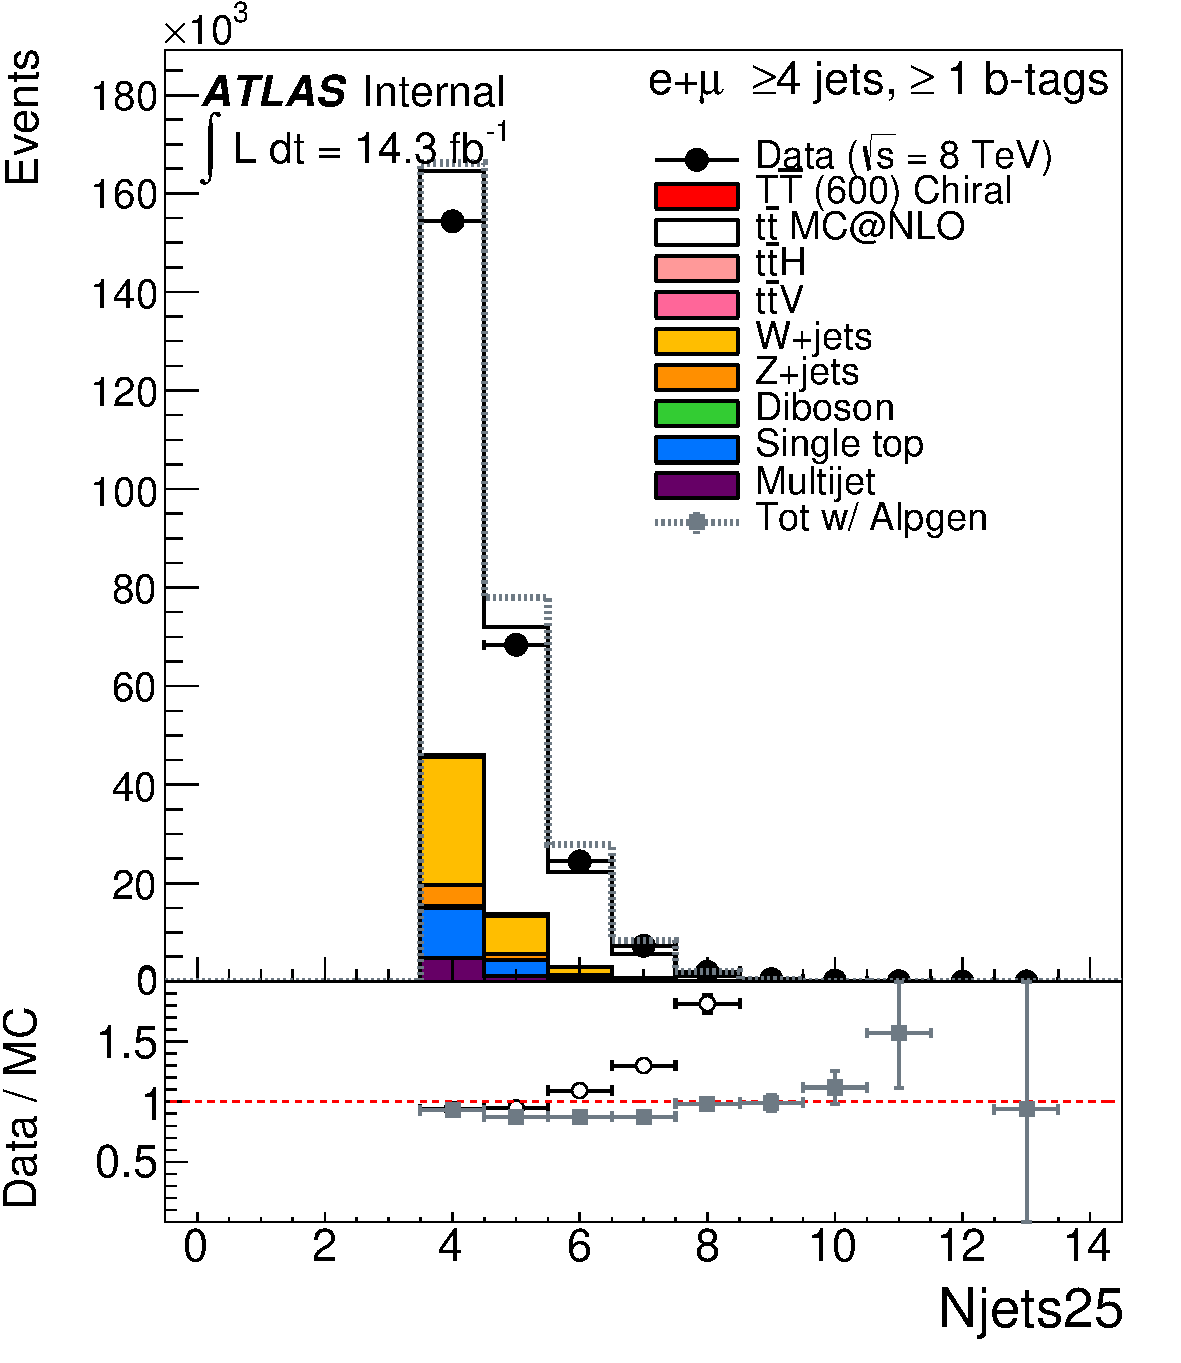
\includegraphics[width=0.8\textwidth]{pics/Njets25_ELEMUON_4jetin1btagin_NOMINAL}

}

\end{minipage}

\end{frame}

\begin{frame}\frametitle{Background and signal modelling}
\centering\myskip

\begin{minipage}{.5\textwidth}\footnotesize\centering
\scriptsize
Yields in the preselection region ``blinded'' as:\\
$\htfj<800\gev$ (*)
\myskip

  \begin{tabular}{l D{;}{\,\pm\,}{-1} } \toprule
 & \multicolumn{1}{c}{ $\geq 4$ jets, $\geq 1$ $b$-tags } 		 \\ \midrule 
 Multi-jet  & 6264;74 \\ 
 Single top  & 14375;107 \\ 
 Diboson  & 548;12 \\ 
 $Z$+jets  & 5804;146 \\ 
 $W$+jets  & 35921;525 \\ 
 $t\bar{t}$V & 680;2 \\ 
 $t\bar{t}$H (125)  & 220;1 \\ 
 $t\bar{t}$ MC@NLO  & 202042;285 \\ 
\midrule 
  Tot Bkg w/ MC@NLO  & 265854;629 \\ \midrule 
\rowcolor{LightCyan}   $T\bar{T}$ (600) chiral  & 36;2 \\ 
 Data  & 256993;507 \\ 
\bottomrule\end{tabular}


\myskip
(*) $\htfj = \pT(l) + \met + \sum_{j = 1}^{\rm 4}\pT(j)$
\end{minipage}\begin{minipage}{.5\textwidth}\footnotesize\centering

\begin{itemize}
\item \TTbar\ singlet production generated with {\tt PROTOS}+{\tt PYTHIA}
\item Branching ratio to each decay mode  ($Wb$, $Zt$ and $Ht$) is set to  1/3
\item Events are reweighted at the analysis level in order to reproduce any desired branching ratio configuration
\item $m_{T}$ values generated from $350\gev$ to $850\gev$ in steps of $50\gev$
\item $m_H=125\gev$, all Higgs boson decay modes are considered
\item NNLO theoretical cross section
\end{itemize}

\tiny
\begin{tabular}{c c c c}
\toprule
 $m_{T}$ ($\gev$) & $BR(T \to Wb)$ & $BR(T \to Zt)$ & $BR(T \to Ht)$\\
 & \multicolumn{3}{c}{Singlet} \\
600 	&  0.494 	&  0.194 	&  0.312	\\
\midrule
&  \multicolumn{3}{c}{Doublet} \\
600 	& 0.000 	&  0.383 	&  0.617 	\\ 	
\bottomrule
\end{tabular}

\end{minipage}


\end{frame}

\begin{frame}\frametitle{Systematic uncertainties - Shape and Norm}
\centering\myskip\scriptsize

\begin{tabular}{lcccc}
\toprule
Systematic uncertainty & \multicolumn{2}{c}{ \wbx\  } & \multicolumn{2}{c}{ \htx\  }\\
 & Status  & Components & Status  & Components\\
\midrule
Luminosity                  &  N & 1 &  N & 1\\
Lepton ID+reco+trigger      &  N & 1 &  N & 1\\
Jet vertex fraction efficiency & SN & 1 & SN & 1\\
\rowcolor{TabLight}Jet energy scale            & SN & 1 & SN & 8\\
Jet energy resolution       & SN & 1 & SN & 1\\
%Jet mass scale               & - & -\\
%Jet mass resolution      & - & -\\
\rowcolor{TabLight}$b$-tagging efficiency      & SN & 9 & SN & 9\\
$c$-tagging efficiency      & SN & 5 & SN & 5\\
Light jet-tagging efficiency    & SN & 1 & SN & 1\\
$t\bar{t}$ cross section    &  N & 1 &  N & 1\\
$t\bar{t}V$ cross section   &  N & 1 &  N & 1\\
$t\bar{t}H$ cross section   & - & - &  N & 1\\
Single top cross section    &  N & 1 &  N & 1\\
Dibosons cross section      &  N & 1 &  N & 1\\
$W$+jets normalization      &  N & 5 &  - & -\\
$Z$+jets normalization      &  N & 1 &  - & -\\
$V$+jets normalization      &  - & - &  N & 1\\
Multijet normalization      &  - & - &  N & 1\\
\rowcolor{TabLight}$t\bar{t}$ modelling        & SN & 3 & SN & 3\\
$V$+jets modelling         & SN & 1 &  - & -\\
$t\bar{t}$+heavy-flavour fractions &  - & -& N & 1\\
%$\TT$ modelling        & - & -\\
\bottomrule
\end{tabular}

\end{frame}


%----------------------------------
\section{Search for \TTbar\ decaying to $Wb+X$}
%----------------------------------
\begin{frame}\frametitle{Strategy}
\centering\myskip

\begin{minipage}{.25\textwidth}\centering
\footnotesize

$$\TTbar\to WbWb$$ 
like $$\ttbar\to WbWb$$

\myskip
\myskip


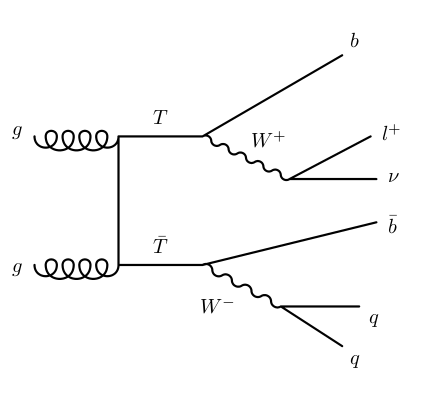
\includegraphics[width=1.15\textwidth]{pics/feyn_wbwb}


\end{minipage}\begin{minipage}{.75\textwidth}\centering
\vskip-5ex
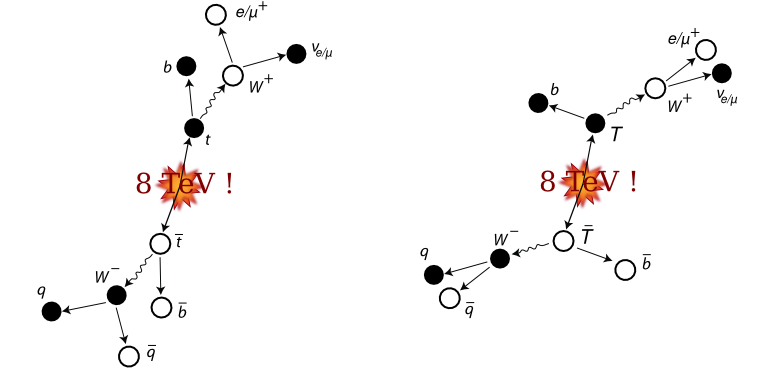
\includegraphics[width=1.\textwidth]{../wbx_analysis_14ifb/figures/kin.png}

different {\cccolor boosted kinematics}\\
{\LARGE $\Downarrow$}\\
reconstruct the $W$ boson from hadronic decay\\
{\LARGE $\swarrow\searrow$}\\
\begin{minipage}{.3\textwidth}\centering
merged jets\\
\wi
\end{minipage}\begin{minipage}{.3\textwidth}\centering
close-by jets\\
\wii
\end{minipage}

\end{minipage}

\end{frame}

%%%%%%%%%%%%%%%%%%%%%%%%%
%%%
%%%%%%%%%%%%%%%%%%%%%%%%%
\begin{frame}\frametitle{$W$ boson reconstruction}
\centering\footnotesize

\begin{minipage}{.34\textwidth}\centering

{\cccolor \large \wi}

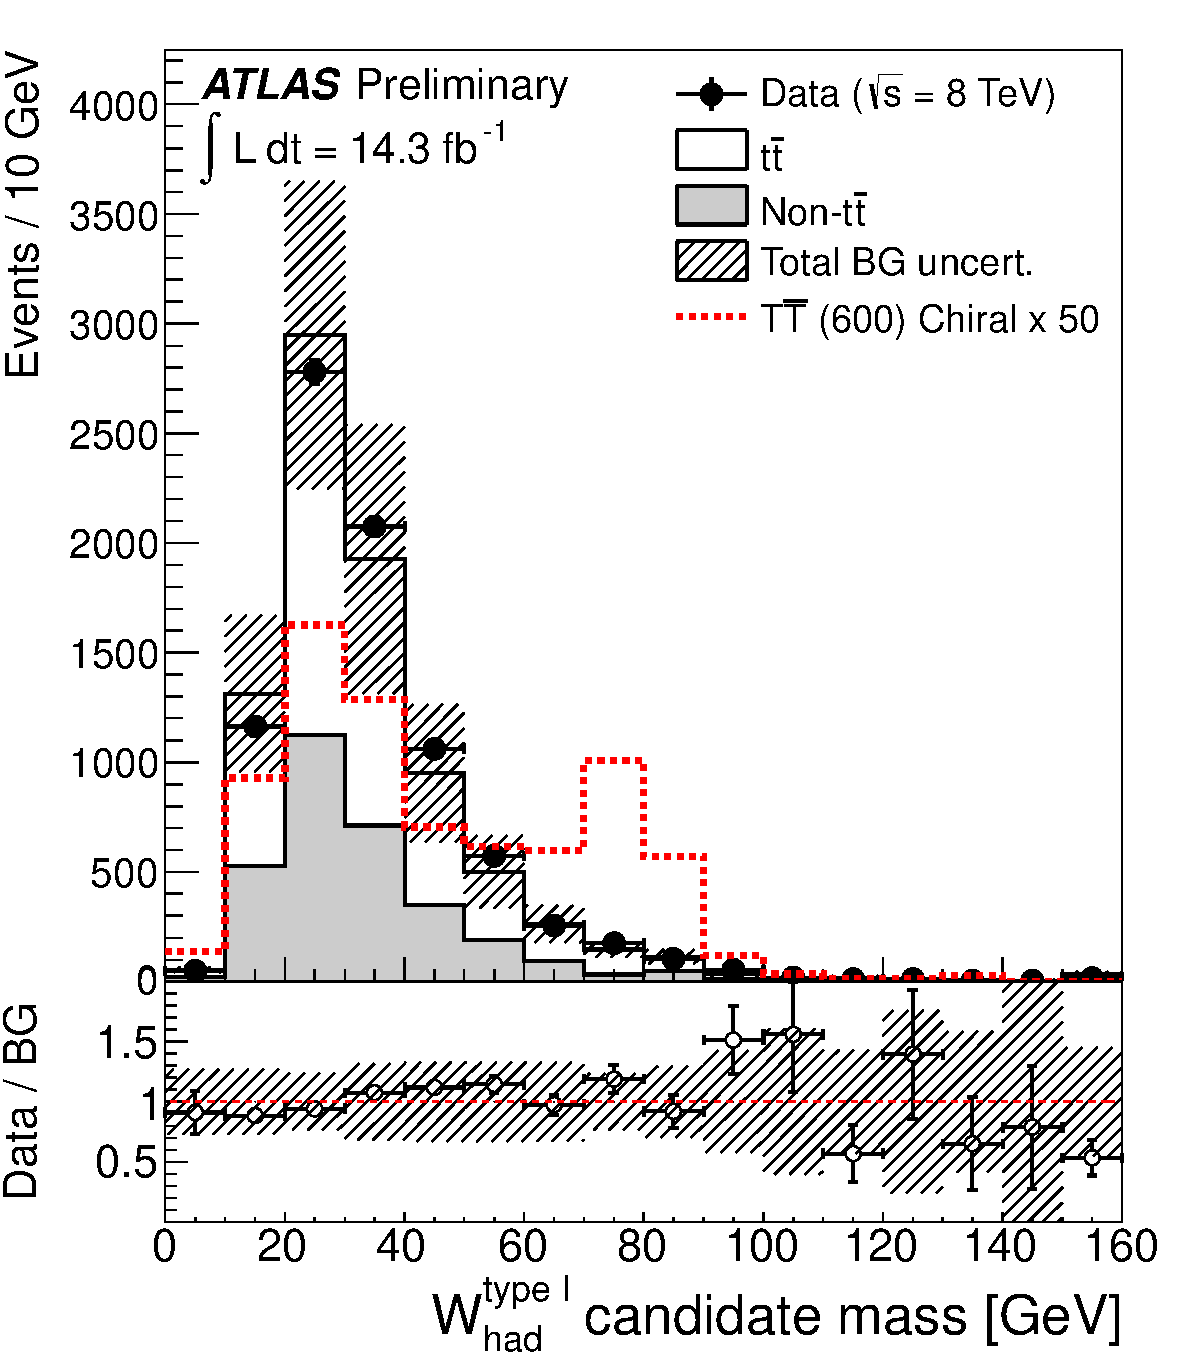
\includegraphics[width=1.\textwidth]{pics/VLQAna_WbX_WpreselType1_M_ELEMUON_preselW_NOMINAL}
\end{minipage}\begin{minipage}{.31\textwidth}\centering

%$$\Rightarrow$$
%$$\Leftarrow$$
{ \footnotesize
\myskip

\hskip-3ex
\begin{tabular}{p{.05cm} c}
%\toprule
\ldelim\{{5}{5ex}[] & \\
                      & one jet \\
                      & $\pt>250\gev$ \\
                      & $60<M<120\gev$ \\
& \\
\end{tabular}

\myskip

\hskip-3ex
\begin{tabular}{c p{.05cm}}
%\toprule
 & \rdelim\}{7}{7ex}[]\\
 no \wi & \\
 di-jet system &\\
 $\dr(j,j)<0.8$&  \\
 $\pt>200\gev$&  \\
 $60<M<120\gev$&  \\
& \\
\end{tabular}
}


\end{minipage}\begin{minipage}{.35\textwidth}\centering

{\cccolor \large \wii}

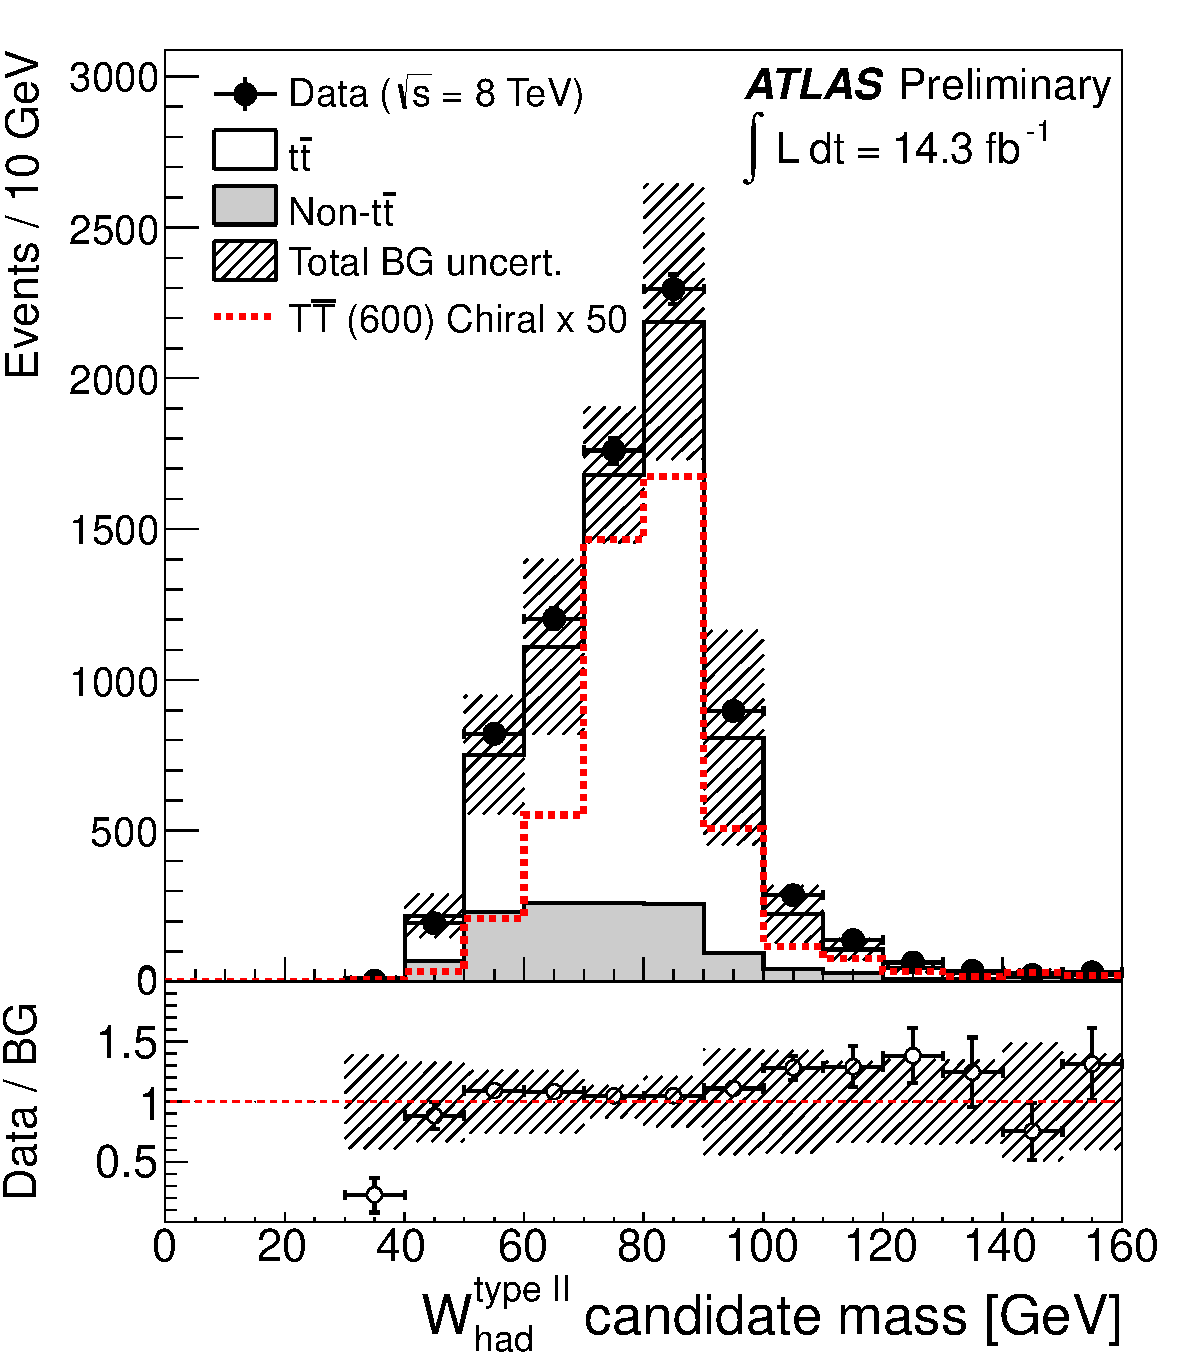
\includegraphics[width=1.\textwidth]{pics/VLQAna_WbX_WpreselType2_M_ELEMUON_preselW_NOMINAL}
\end{minipage}

\myskip

{\cccolor \wlep\ } reconstructed using {\cccolor lepton} and {\cccolor ``neutrino''}:\\
$p_X, p_Y$ from \met, $p_Z$ from $M_W^2 = (P_l + P_{\nu})^2$


\end{frame}

%%%%%%%%%%%%%%%%%%%%%%%%%
%%%
%%%%%%%%%%%%%%%%%%%%%%%%%
\begin{frame}\frametitle{Event selection}
\centering\footnotesize

\begin{minipage}{.5\textwidth}\centering
\begin{tabular}{ll}
\toprule
\multicolumn{2}{c}{\loose\ selection}\\
 SR0 & Preselection  \\
 SR1 & +\hskip5ex$\geq 1~W_{\rm had}$ candidates \\
 SR2 & +\hskip5ex$\htfj>800\gev$ \\
 SR3 & +\hskip5ex $\pt(b_1) > 160\gev$\\
 SR4 & +\hskip5ex$\pt(b_2) >80\gev$ \\
 SR5 & +\hskip5ex$\Delta R(\ell,\nu)<1.2$ \\
\bottomrule
\toprule
\multicolumn{2}{c}{\tight\  selection} \\
 SR5 & \loose\ selection \\
 SR6 &  +\hskip5ex min$\Delta R(\ell,b)>1.4$\\
 SR7 & +\hskip5ex min$\Delta R(W_{\rm had},b)>1.4$ \\
\bottomrule
\end{tabular}

%N.B. \bjet s are the two jets with highest \btag\ weight

\end{minipage}\begin{minipage}{.5\textwidth}\centering



\begin{pgfpicture}{0.0\textwidth}{0.0\textheight}{1.\textwidth}{.6\textwidth}
   \begin{pgftranslate}{\pgfpoint{0.05\textwidth}{-0.12\textheight}}
\pgfdeclareimage[interpolate=true,width=.95\textwidth]{htall}{pics/HTAll_ELEMUON_cutflow1_NOMINAL.pdf}
\pgfdeclareimage[interpolate=true,width=.95\textwidth]{jetptb1}{pics/JetPtB1_ELEMUON_cutflow12_NOMINAL.pdf}
\pgfdeclareimage[interpolate=true,width=.95\textwidth]{jetptb2}{pics/JetPtB2_ELEMUON_cutflow123_NOMINAL.pdf}
\pgfdeclareimage[interpolate=true,width=.95\textwidth]{nwhad}{pics/nWhad_ELEMUON_cutflow0_NOMINAL_logscale.pdf}
\pgfdeclareimage[interpolate=true,width=.95\textwidth]{mrecoT}{pics/VLQAna_WbX_1W_MWb_4_ELEMUON_cutflow1234567_NOMINAL.pdf}
\pgfdeclareimage[interpolate=true,width=.95\textwidth]{mrecoL}{pics/VLQAna_WbX_1W_MWb_4_ELEMUON_cutflow12345_NOMINAL.pdf}
\pgfdeclareimage[interpolate=true,width=.95\textwidth]{drlep}{pics/VLQAna_WbX_DRLepMet_ELEMUON_cutflow1234_NOMINAL.pdf}
\pgfdeclareimage[interpolate=true,width=.95\textwidth]{mindrl}{pics/VLQAna_WbX_MinDRlb_ELEMUON_cutflow12345_NOMINAL.pdf}
\pgfdeclareimage[interpolate=true,width=.95\textwidth]{mindrw}{pics/VLQAna_WbX_MinDRWb_ELEMUON_cutflow123456_NOMINAL.pdf}
%\pgfputat{\pgfxy(0.0,0.0)}{\pgfbox[left,base]{\pgfuseimage{mindr}}}
 \pgfsetlinewidth{1.pt}
 \usebeamercolor[bg]{head/foot boxes}
\only<1>{
 \pgfrect[stroke]{\pgfxy(-6,3.82)}{\pgfxy(5,0.35)}
 \pgfstroke
\pgfputat{\pgfxy(0.0,-0.8)}{\pgfbox[left,base]{\pgfuseimage{nwhad}}}
 {\usebeamercolor[fg]{head/foot boxes}
 \pgfline{\pgfxy(1.8,0.)}{\pgfxy(1.8,5.5)} }
}
\only<2>{
 \pgfrect[stroke]{\pgfxy(-6,3.46)}{\pgfxy(5,0.35)}
 %\pgfline{\pgfxy(1.55,1.5)}{\pgfxy(1.55,3.5)} 
 \pgfstroke
\pgfputat{\pgfxy(0.0,-0.8)}{\pgfbox[left,base]{\pgfuseimage{htall}}}
 {\usebeamercolor[fg]{head/foot boxes}
 \pgfline{\pgfxy(1.8,0.)}{\pgfxy(1.8,5.5)} }
}
\only<3>{
% \pgfrect[stroke]{\pgfxy(-6,3.1)}{\pgfxy(5,0.35)}
 \pgfrect[stroke]{\pgfxy(-6,2.74)}{\pgfxy(5,0.7)}
 \pgfstroke
 \pgfputat{\pgfxy(0.0,-0.8)}{\pgfbox[left,base]{\pgfuseimage{jetptb1}}}
 {\usebeamercolor[fg]{head/foot boxes}
 \pgfline{\pgfxy(1.8,0.)}{\pgfxy(1.8,5.5)} }
}
\only<4>{
 \pgfrect[stroke]{\pgfxy(-6,2.45)}{\pgfxy(5,0.35)}
 %\pgfline{\pgfxy(1.55,1.5)}{\pgfxy(1.55,3.5)} 
 \pgfstroke
\pgfputat{\pgfxy(0.0,-0.8)}{\pgfbox[left,base]{\pgfuseimage{drlep}}}
 {\usebeamercolor[fg]{head/foot boxes}
 \pgfline{\pgfxy(1.8,0.)}{\pgfxy(1.8,5.5)} }
}
\only<5>{
 \pgfrect[stroke]{\pgfxy(-6,1.15)}{\pgfxy(5,0.35)}
 %\pgfline{\pgfxy(1.55,1.5)}{\pgfxy(1.55,3.5)} 
 \pgfstroke
\pgfputat{\pgfxy(0.0,-0.8)}{\pgfbox[left,base]{\pgfuseimage{mindrl}}}
 {\usebeamercolor[fg]{head/foot boxes}
 \pgfline{\pgfxy(1.8,0.)}{\pgfxy(1.8,5.5)} }
}
\only<6>{
 \pgfrect[stroke]{\pgfxy(-6,0.8)}{\pgfxy(5,0.35)}
 %\pgfline{\pgfxy(1.55,1.5)}{\pgfxy(1.55,3.5)} 
 \pgfstroke
\pgfputat{\pgfxy(0.0,-0.8)}{\pgfbox[left,base]{\pgfuseimage{mindrw}}}
 {\usebeamercolor[fg]{head/foot boxes}
 \pgfline{\pgfxy(1.8,0.)}{\pgfxy(1.8,5.5)} }
}
   \end{pgftranslate}

\end{pgfpicture}

\end{minipage}

\end{frame}


%%%%%%%%%%%%%%%%%%%%%%%%%
%%%
%%%%%%%%%%%%%%%%%%%%%%%%%
\begin{frame}\frametitle{Comparison data vs prediction}
\centering\footnotesize

\begin{minipage}{.5\textwidth}\centering

{\it (before unblinding)}\\
Check agreement between data and background prediction

{\Large$\Downarrow$}

Define regions depleted in signal

\myskip

\scriptsize
\begin{tabular}{l*{1}{r@{ $\pm$ }r@{ }l}}
\toprule
 & \multicolumn{3}{c}{\loose\ but $\Delta R(\ell,\nu)>1.2$}\\
\midrule
$t\bar{t'} (600\GeV)$ & $18.47$ & $1.48$ & $^{+1.09}_{-1.64}$\\
\midrule
$t\bar{t}$ & $173.13$ & $8.82$ & $^{+46.92}_{-48.59}$\\
$W$+jets & $30.64$ & $9.78$ & $^{+13.74}_{-12.43}$\\
$Z$+jets & $11.68$ & $5.93$ & $^{+5.89}_{-6.96}$\\
Diboson & $0.29$ & $0.19$ & $^{+0.17}_{-0.17}$\\
Single top & $21.46$ & $2.54$ & $^{+2.60}_{-2.54}$\\
$t\bar{t}$$V$ & $4.21$ & $0.16$ & $^{+1.33}_{-1.33}$\\
Multijet & $0.49$ & $0.91$ & $ \pm\ 0.25$\\
\midrule
Total bkg. & $241.90 $ & $ 14.70$ & $ ^{+53.57}_{-55.95}$\\
\midrule
Data & \multicolumn{3}{c}{$250$}\\
\bottomrule
\end{tabular}


\end{minipage}\begin{minipage}{.5\textwidth}\centering

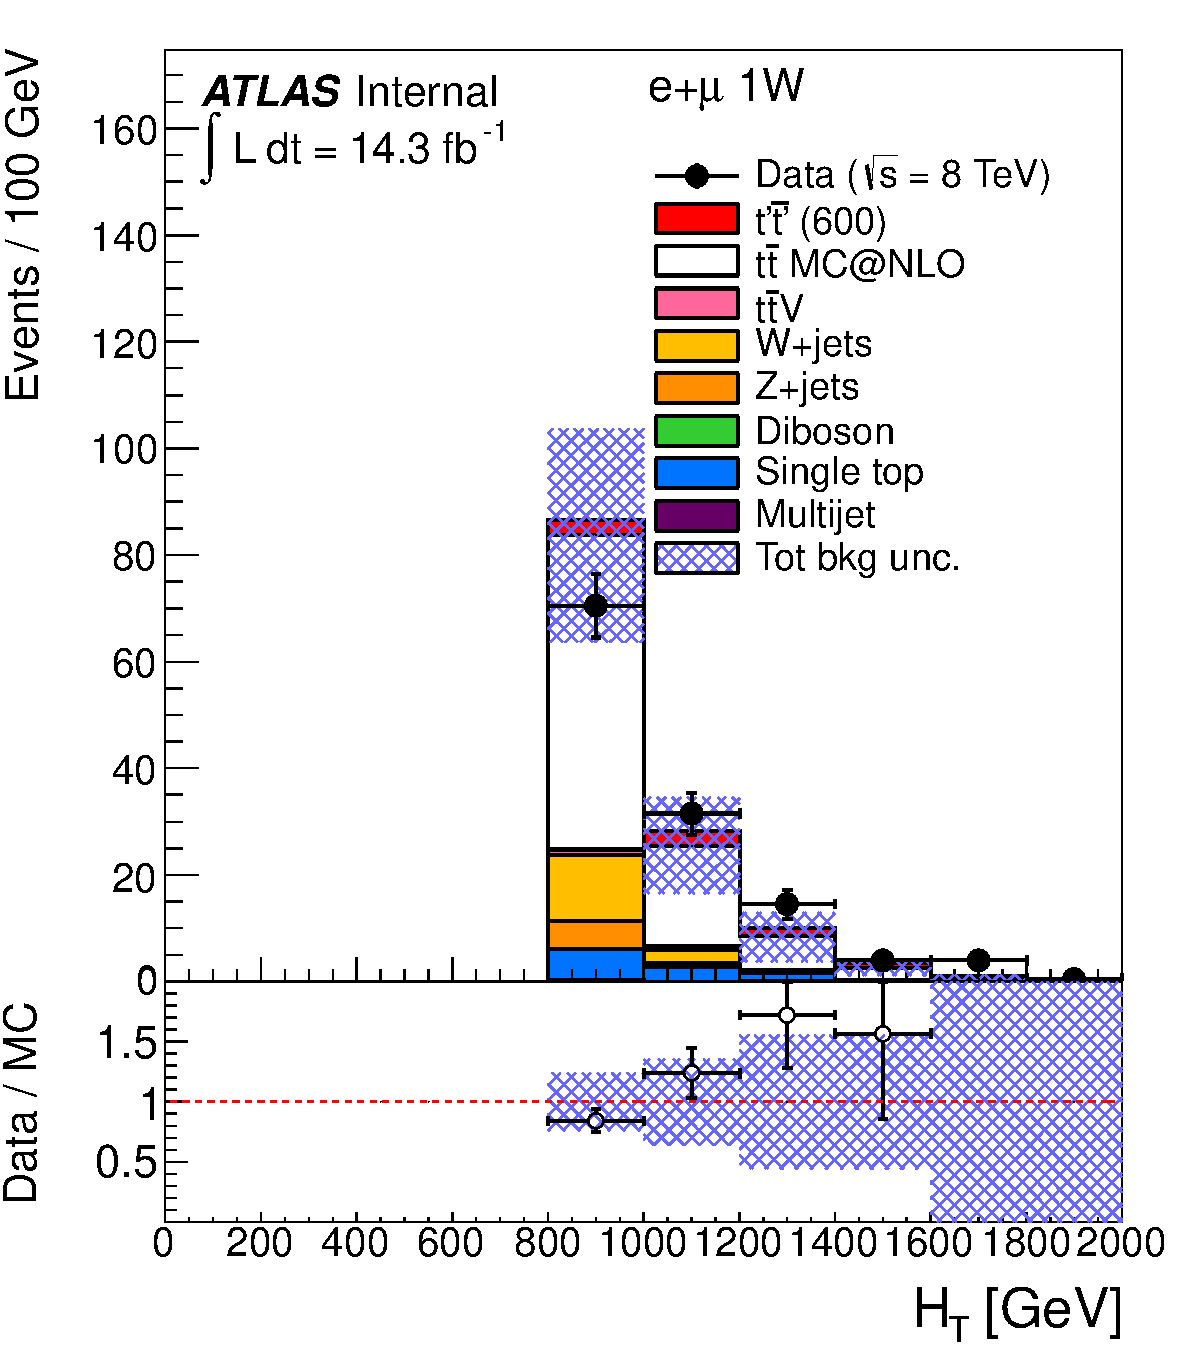
\includegraphics[width=.5\textwidth]{pics/HTAll_ELEMUONCR3_1W_NOMINAL.pdf}
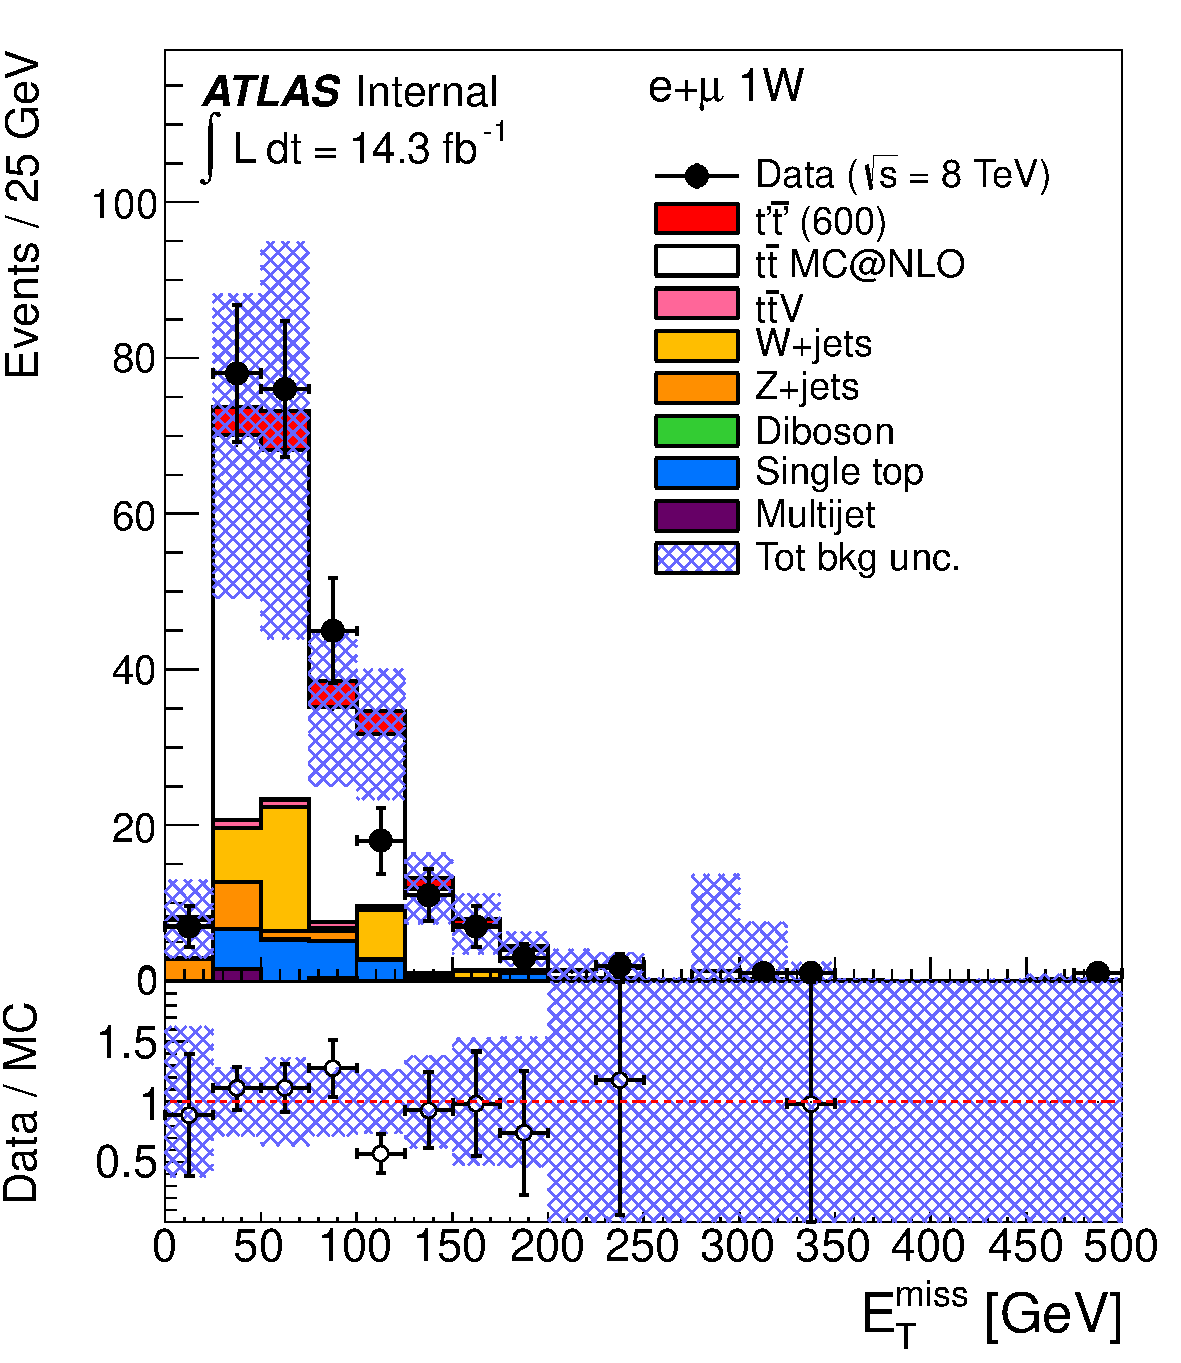
\includegraphics[width=.5\textwidth]{pics/MET_ELEMUONCR3_1W_NOMINAL.pdf}\\
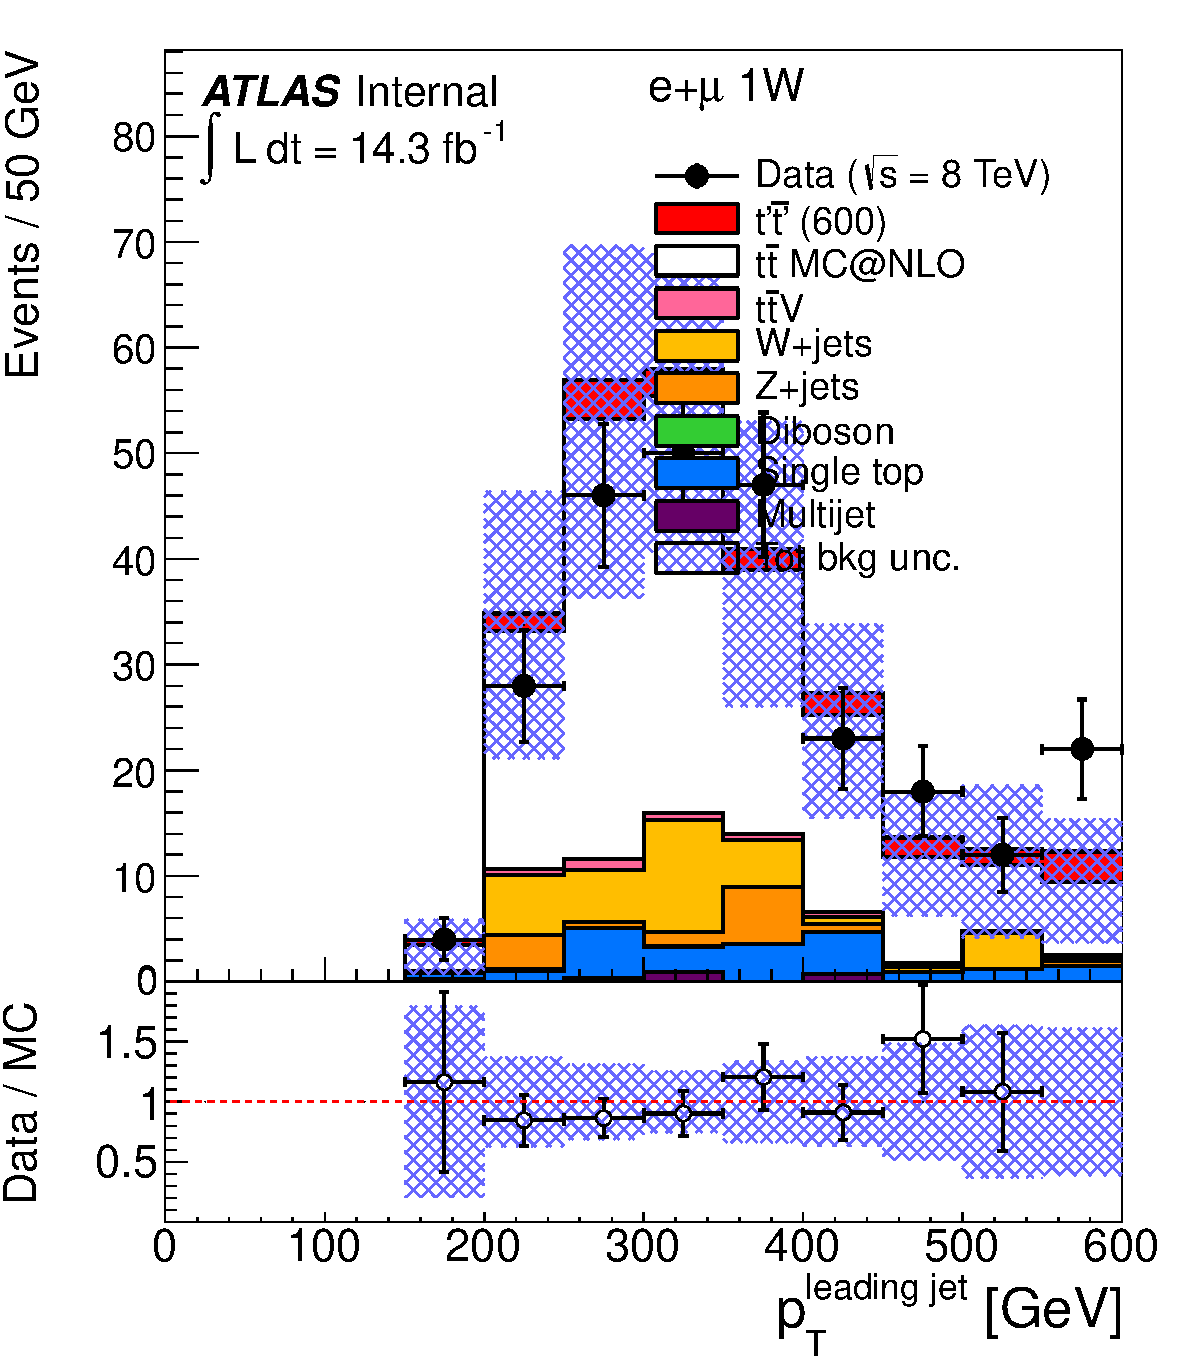
\includegraphics[width=.5\textwidth]{pics/JetPt1_ELEMUONCR3_1W_NOMINAL.pdf}
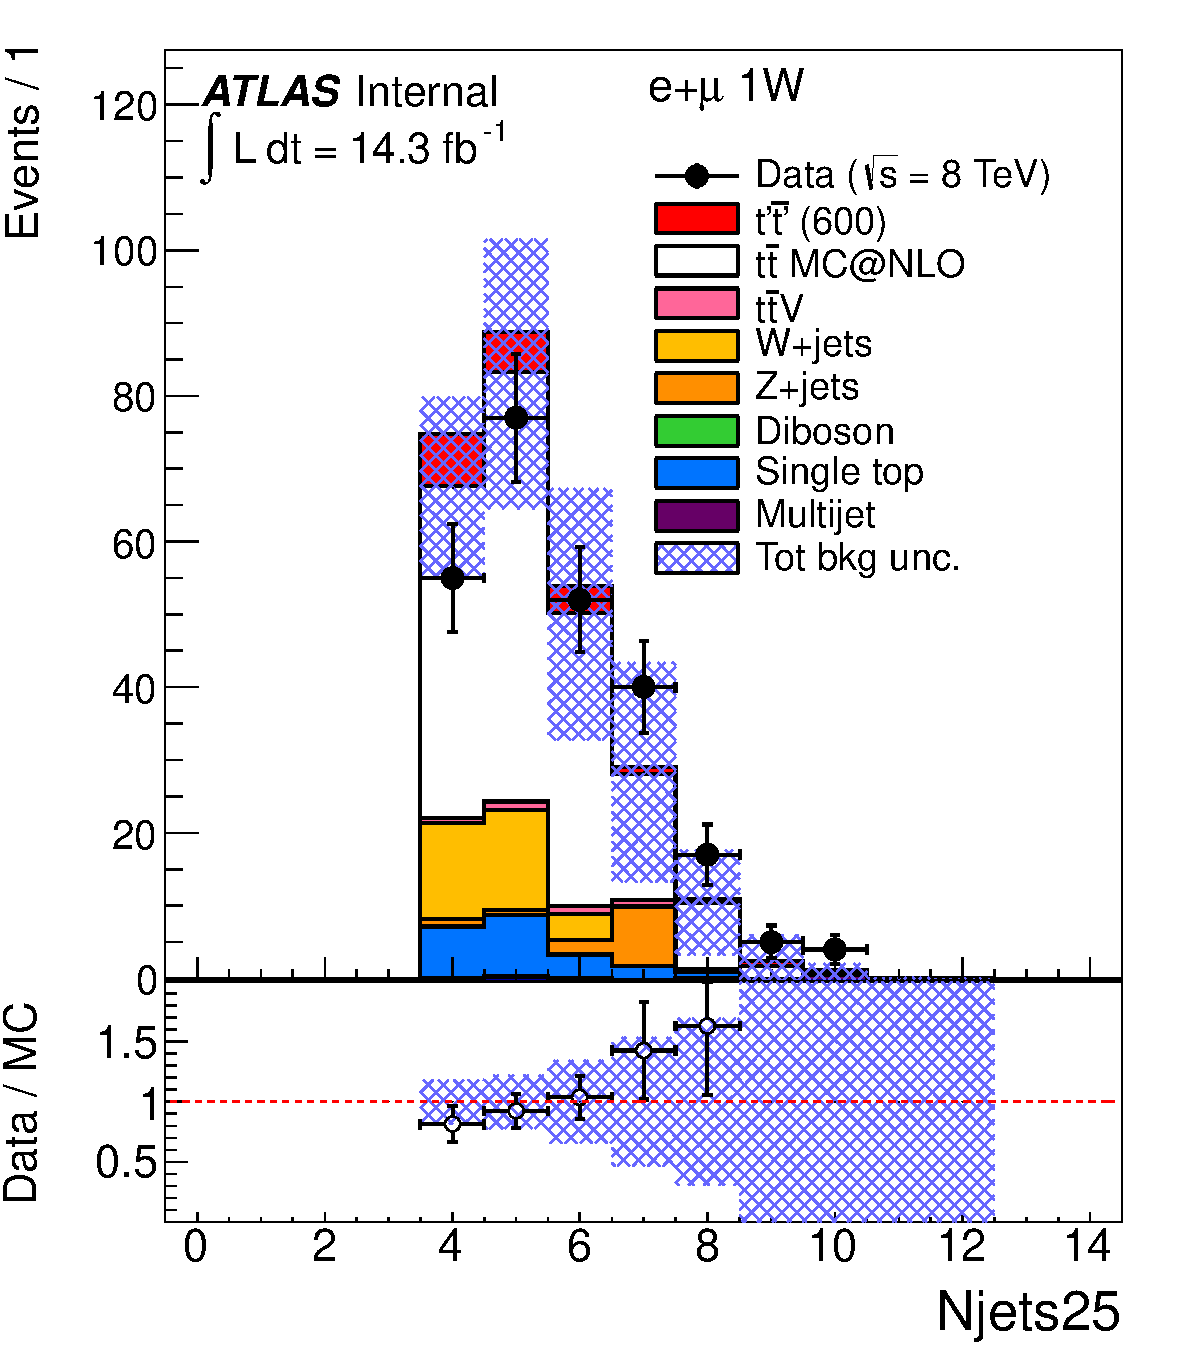
\includegraphics[width=.5\textwidth]{pics/Njets25_ELEMUONCR3_1W_NOMINAL.pdf}

\end{minipage}

\end{frame}


%%%%%%%%%%%%%%%%%%%%%%%%%
%%%
%%%%%%%%%%%%%%%%%%%%%%%%%
\begin{frame}\frametitle{Signal to background discrimination}
\centering\scriptsize

\begin{minipage}{.6\textwidth}\centering

\hskip-5ex
\begin{tabular}{p{0.05cm} p{0.05cm}}
\\
\\
%\parbox[t]{2mm}{\multirow{5}{*}{\rotatebox[origin=c]{90}{rota}}}& \ldelim\{{5}{5ex} \\
\multirow{5}{*}{\rotatebox[origin=c]{90}{\cccolor merged}}& \ldelim\{{5}{5ex} \\
\\
\\
\\
\\
\\
\\
\\
\\
\\
\\
\end{tabular}\begin{tabular}{l  D{;}{\,\pm\,}{-1} D{;}{\,\pm\,}{-1} }
    \toprule
    & \multicolumn{1}{c}{\loose} 
    & \multicolumn{1}{c}{\tight}  \\\midrule
$t\bar{t}$    & 264;80 & 10;6 \\
$t\bar{t}V$   &  5.1;1.8 & 0.5;0.2 \\
$W$+jets   &  16;11 & 6;5\\
$Z$+jets   &  1.1;1.4 & 0.2;0.5 \\
Single top   &  30;7 & 4.4;1.6  \\
Dibosons &  0.21;0.15 & 0.06;0.05 \\
\midrule
Tot.Bkg.  & 317;90 & 21;9 \\
Data& 348 & 37  \\
%Data& \multicolumn{1}{c}{348\,\phantom{$\pm$}} & 37  \\
\midrule
$T\bar{T}(600\GeV)$ \\
Chiral $t'$&  88;10 & 54;7 \\
$T$ Singlet      & 41;4 & 20.3;2.2 \\
\bottomrule\end{tabular}

\myskip

\end{minipage}\begin{minipage}{.4\textwidth}\centering

\myskip

\footnotesize
Discriminating variable $\Rightarrow$ {\cccolor $T$ reconstructed mass}\\
{\large$\Downarrow$}\\
Pair \bjet s and $W$ boson candidates in order to get\\
min$\Delta(M_{\rm lep},M_{\rm had})$

%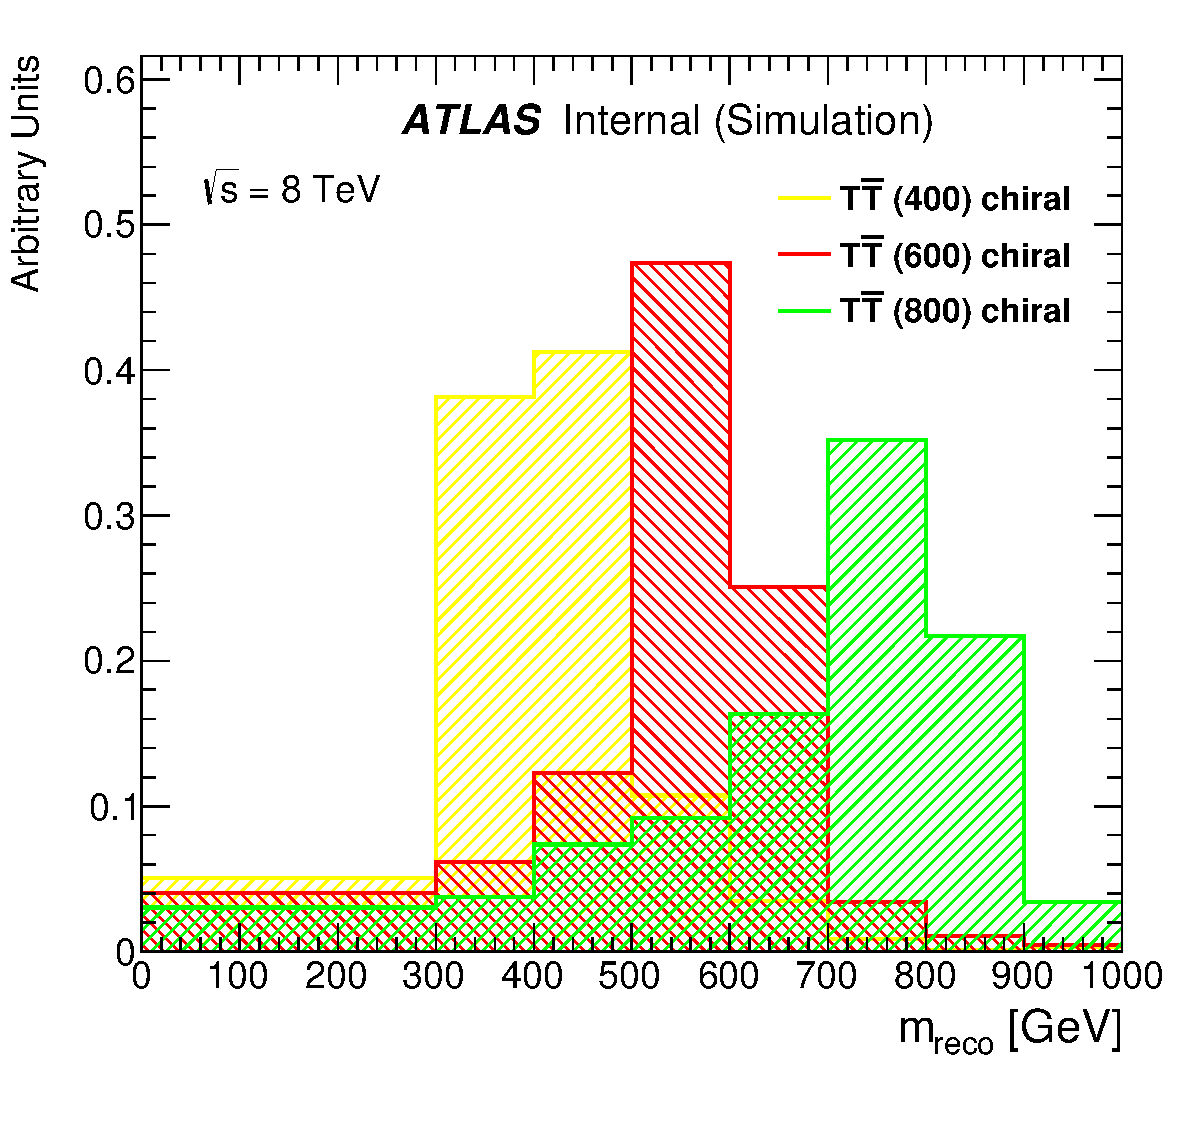
\includegraphics[width=.8\textwidth]{pics/VLQAna_WbX_1W_MWb_4_ELEMUONloose_1W_NOMINAL_VLTtt.pdf}\\
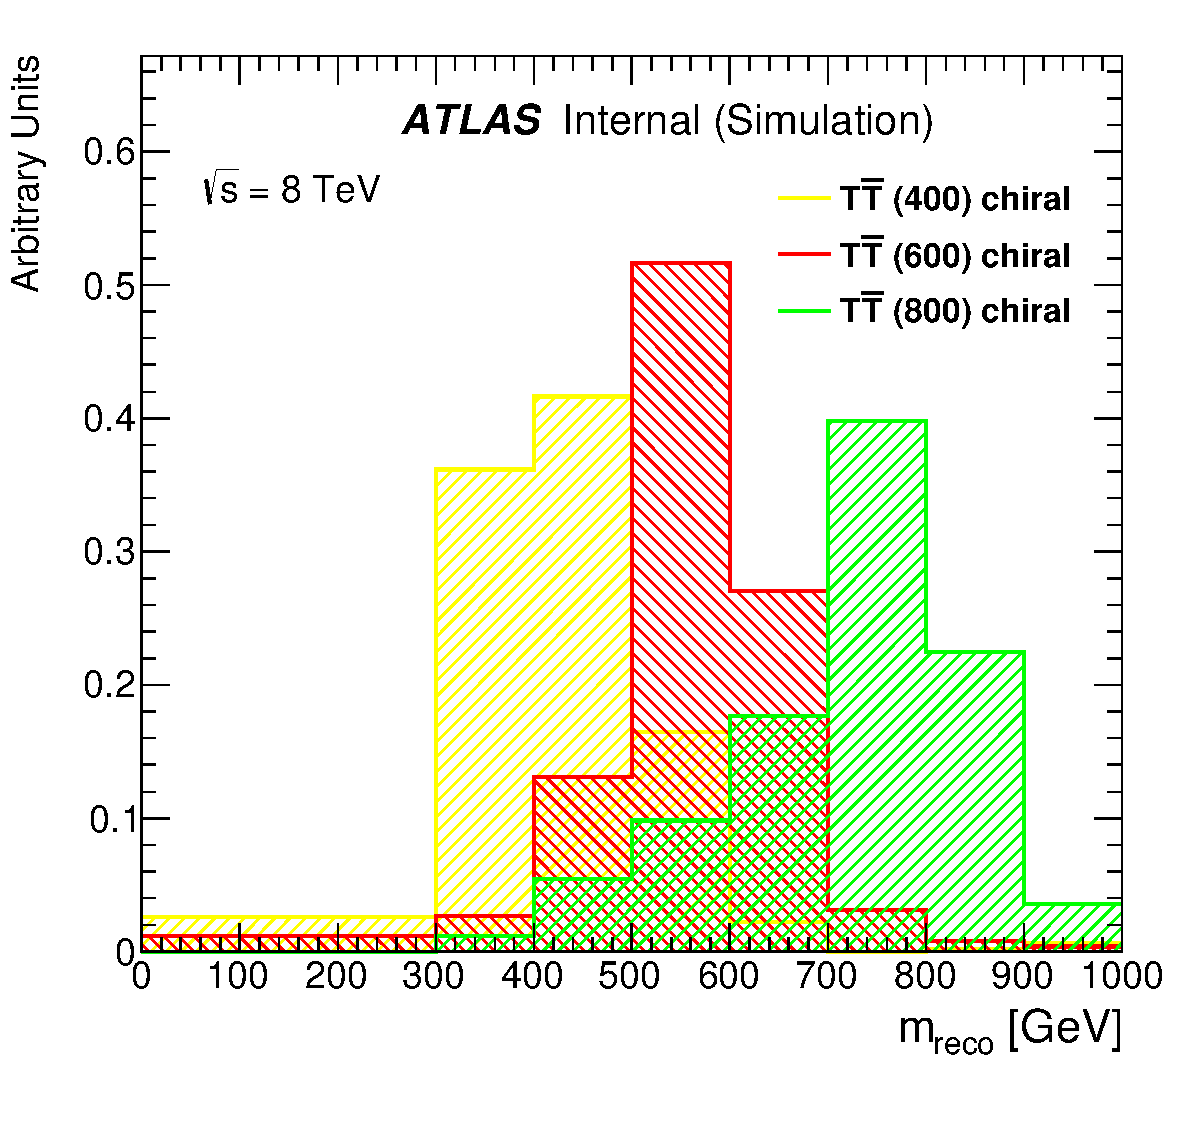
\includegraphics[width=.9\textwidth]{pics/VLQAna_WbX_1W_MWb_4_ELEMUONtight_1W_NOMINAL_VLTtt.pdf}
\end{minipage}

\end{frame}



%%%%%%%%%%%%%%%%%%%%%%%%%
%%%
%%%%%%%%%%%%%%%%%%%%%%%%%
\begin{frame}\frametitle{Reconstructed mass}
\centering\footnotesize

\begin{minipage}{.5\textwidth}\centering
\begin{tabular}{ll}
\toprule
\multicolumn{2}{c}{\loose\ selection}\\
 SR0 & Preselection  \\
 SR1 & +\hskip5ex$\geq 1~W_{\rm had}$ candidates \\
 SR2 & +\hskip5ex$\htfj>800\gev$ \\
 SR3 & +\hskip5ex $\pt(b_1) > 160\gev$\\
 SR4 & +\hskip5ex$\pt(b_2) >80\gev$ \\
 SR5 & +\hskip5ex$\Delta R(\ell,\nu)<1.2$ \\
\bottomrule
\toprule
\multicolumn{2}{c}{\tight\  selection} \\
 SR5 & \loose\ selection \\
 SR6 &  +\hskip5ex min$\Delta R(\ell,b)>1.4$\\
 SR7 & +\hskip5ex min$\Delta R(W_{\rm had},b)>1.4$ \\
\bottomrule
\end{tabular}

%N.B. \bjet s are the two jets with highest \btag\ weight

\end{minipage}\begin{minipage}{.5\textwidth}\centering



\begin{pgfpicture}{0.0\textwidth}{0.0\textheight}{1.\textwidth}{.6\textwidth}
   \begin{pgftranslate}{\pgfpoint{0.05\textwidth}{-0.12\textheight}}

\pgfdeclareimage[interpolate=true,width=.95\textwidth]{mreco6}{pics/THESIS_c6_cutflow/VLQAna_WbX_1W_MWb_4_ELEMUON_cutflow123456_NOMINAL.pdf}
\pgfdeclareimage[interpolate=true,width=.95\textwidth]{mreco4}{pics/THESIS_c6_cutflow/VLQAna_WbX_1W_MWb_4_ELEMUON_cutflow1234_NOMINAL.pdf}
\pgfdeclareimage[interpolate=true,width=.95\textwidth]{mreco3}{pics/THESIS_c6_cutflow/VLQAna_WbX_1W_MWb_4_ELEMUON_cutflow123_NOMINAL.pdf}
\pgfdeclareimage[interpolate=true,width=.95\textwidth]{mreco2}{pics/THESIS_c6_cutflow/VLQAna_WbX_1W_MWb_4_ELEMUON_cutflow12_NOMINAL.pdf}
\pgfdeclareimage[interpolate=true,width=.95\textwidth]{mreco1}{pics/THESIS_c6_cutflow/VLQAna_WbX_1W_MWb_4_ELEMUON_cutflow1_NOMINAL.pdf}
\pgfdeclareimage[interpolate=true,width=.95\textwidth]{mrecoT}{pics/VLQAna_WbX_1W_MWb_4_ELEMUON_cutflow1234567_NOMINAL.pdf}
\pgfdeclareimage[interpolate=true,width=.95\textwidth]{mrecoL}{pics/VLQAna_WbX_1W_MWb_4_ELEMUON_cutflow12345_NOMINAL.pdf}
%\pgfputat{\pgfxy(0.0,0.0)}{\pgfbox[left,base]{\pgfuseimage{mindr}}}
 \pgfsetlinewidth{1.pt}
 \usebeamercolor[bg]{head/foot boxes}
\only<1>{
 \pgfrect[stroke]{\pgfxy(-6,3.82)}{\pgfxy(5,0.35)}
 %\pgfline{\pgfxy(1.55,1.5)}{\pgfxy(1.55,3.5)} 
 \pgfstroke
\pgfputat{\pgfxy(0.0,-0.8)}{\pgfbox[left,base]{\pgfuseimage{mreco1}}}
}
\only<2>{
 \pgfrect[stroke]{\pgfxy(-6,3.46)}{\pgfxy(5,0.35)}
 %\pgfline{\pgfxy(1.55,1.5)}{\pgfxy(1.55,3.5)} 
 \pgfstroke
\pgfputat{\pgfxy(0.0,-0.8)}{\pgfbox[left,base]{\pgfuseimage{mreco2}}}
}
\only<3>{
 \pgfrect[stroke]{\pgfxy(-6,3.1)}{\pgfxy(5,0.35)}
 %\pgfline{\pgfxy(1.55,1.5)}{\pgfxy(1.55,3.5)} 
 \pgfstroke
\pgfputat{\pgfxy(0.0,-0.8)}{\pgfbox[left,base]{\pgfuseimage{mreco3}}}
}
\only<4>{
 \pgfrect[stroke]{\pgfxy(-6,2.74)}{\pgfxy(5,0.35)}
 %\pgfline{\pgfxy(1.55,1.5)}{\pgfxy(1.55,3.5)} 
 \pgfstroke
\pgfputat{\pgfxy(0.0,-0.8)}{\pgfbox[left,base]{\pgfuseimage{mreco4}}}
}
\only<5>{
 \pgfrect[stroke]{\pgfxy(-6,2.45)}{\pgfxy(5,0.35)}
 %\pgfline{\pgfxy(1.55,1.5)}{\pgfxy(1.55,3.5)} 
 \pgfstroke
\pgfputat{\pgfxy(0.0,-0.8)}{\pgfbox[left,base]{\pgfuseimage{mrecoL}}}
}
\only<6>{
 \pgfrect[stroke]{\pgfxy(-6,1.15)}{\pgfxy(5,0.35)}
 %\pgfline{\pgfxy(1.55,1.5)}{\pgfxy(1.55,3.5)} 
 \pgfstroke
\pgfputat{\pgfxy(0.0,-0.8)}{\pgfbox[left,base]{\pgfuseimage{mreco6}}}
}
\only<7>{
 \pgfrect[stroke]{\pgfxy(-6,0.8)}{\pgfxy(5,0.35)}
 %\pgfline{\pgfxy(1.55,1.5)}{\pgfxy(1.55,3.5)} 
 \pgfstroke
\pgfputat{\pgfxy(0.0,-0.8)}{\pgfbox[left,base]{\pgfuseimage{mrecoT}}}
}
   \end{pgftranslate}

\end{pgfpicture}

\end{minipage}

\end{frame}


%%%%%%%%%%%%%%%%%%%%%%%%%
%%%
%%%%%%%%%%%%%%%%%%%%%%%%%
\begin{frame}\frametitle{Most relevant systematic uncertainties}
\centering\footnotesize

\begin{tabular}{l*{3}{c}}
\toprule
 & $\T\bar{\T}$ ($600\gev$) & $t\bar{t}$ & Non-$t\bar{t}$\\
\midrule
Total [\%] & +14/-15 & +59/-59 & +42/-35\\
\midrule
Main contributions [\%] &&&\\
Jet energy scale & +6.6/-8.4 & +15/-15 & +33/-22\\  
$t\bar{t}$ modelling: NLO MC generator & -- & +48/-48 & --\\  
$t\bar{t}$ modelling: PS and fragm & -- & +25/-25 & --\\  
$t\bar{t}$ modelling: ISR/FSR & -- & +8.8/-8.8 & --\\   
\bottomrule
\end{tabular}

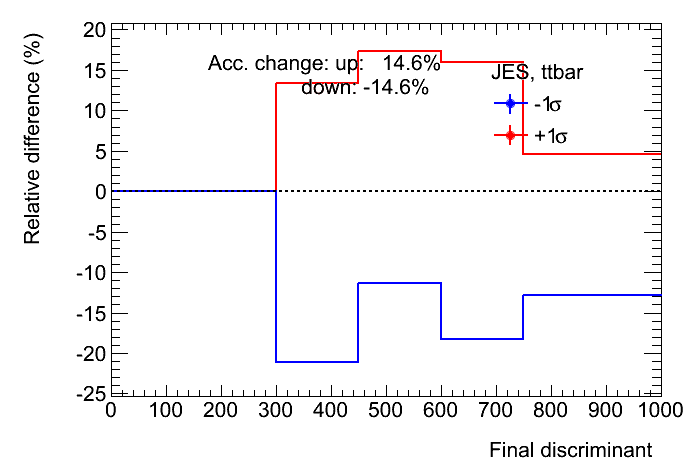
\includegraphics[width=.4\textwidth]{pics/ELEMUON_tight_Bin1_ttbar_JES.png}
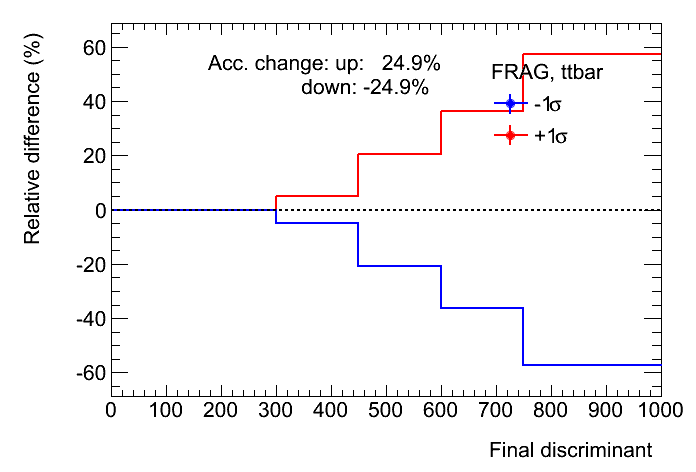
\includegraphics[width=.4\textwidth]{pics/ELEMUON_tight_Bin1_ttbar_FRAG.png}


\end{frame}

%%%%%%%%%%%%%%%%%%%%%%%%%
%%%
%%%%%%%%%%%%%%%%%%%%%%%%%
\begin{frame}\frametitle{Benchmark results}
\centering\footnotesize

\begin{minipage}{.5\textwidth}\centering

Chiral \T/Vector-like $Y(-4/3)$\\

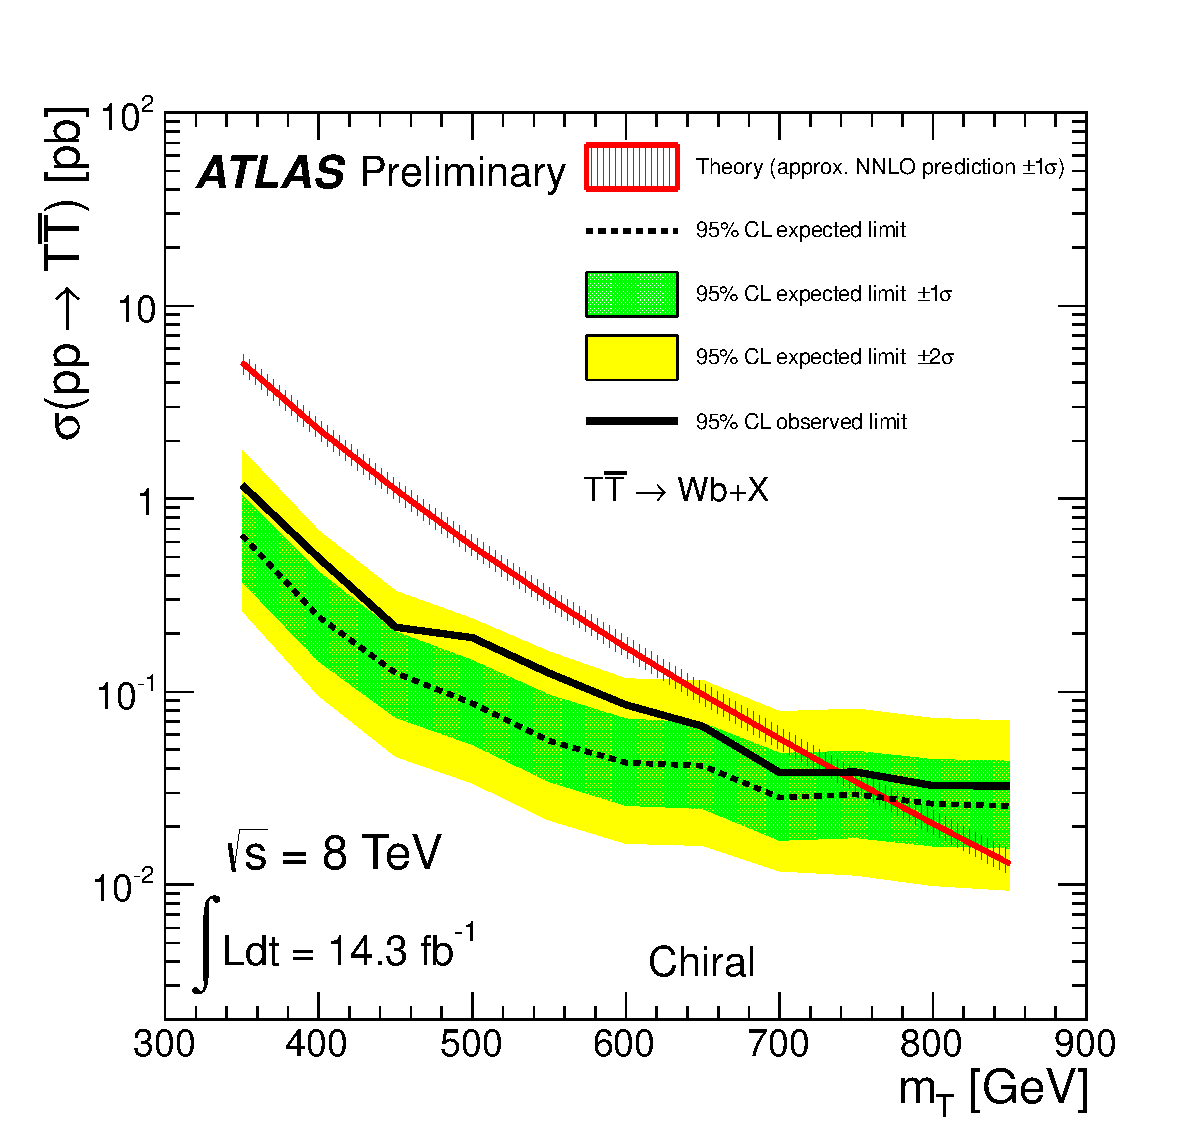
\includegraphics[width=0.9\textwidth]{pics/lim_chiral_bin1_WbX}\\

observed (expected) 95\%  CL limit $m_{\T}>740\,(770)\gev$

\end{minipage}\begin{minipage}{.5\textwidth}\centering

Singlet \T\\

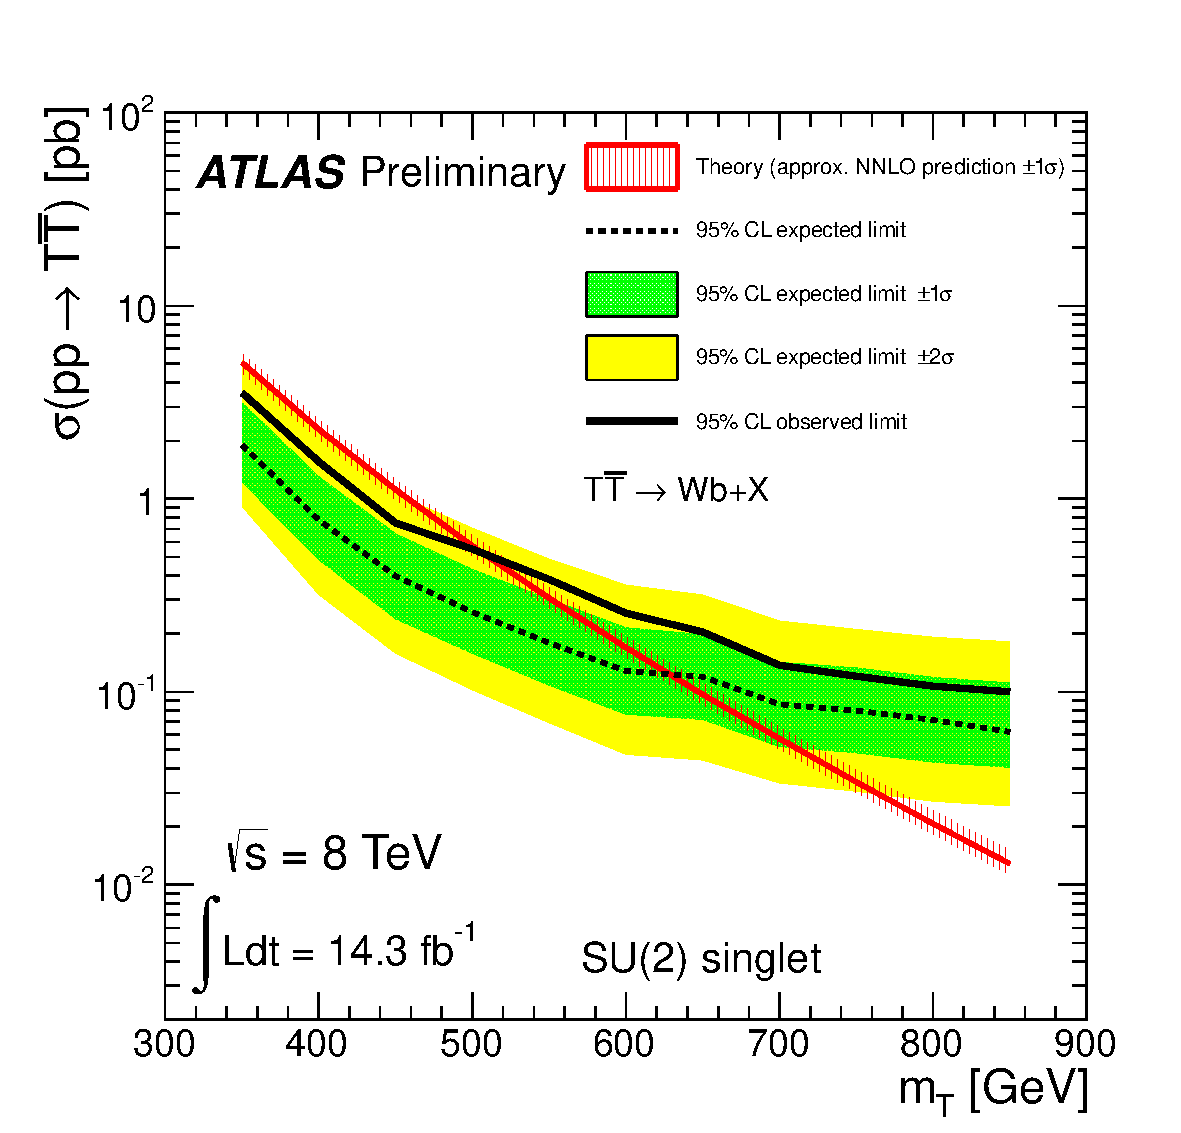
\includegraphics[width=0.9\textwidth]{pics/lim_singlet_bin1_WbX}\\

observed (expected) 95\%  CL  limit 
$m_{\T}>505\,(630)\gev$ 

\end{minipage}


\end{frame}

%%%%%%%%%%%%%%%%%%%%%%%%%
%%%
%%%%%%%%%%%%%%%%%%%%%%%%%
\begin{frame}\frametitle{Model independent results}
\centering\footnotesize

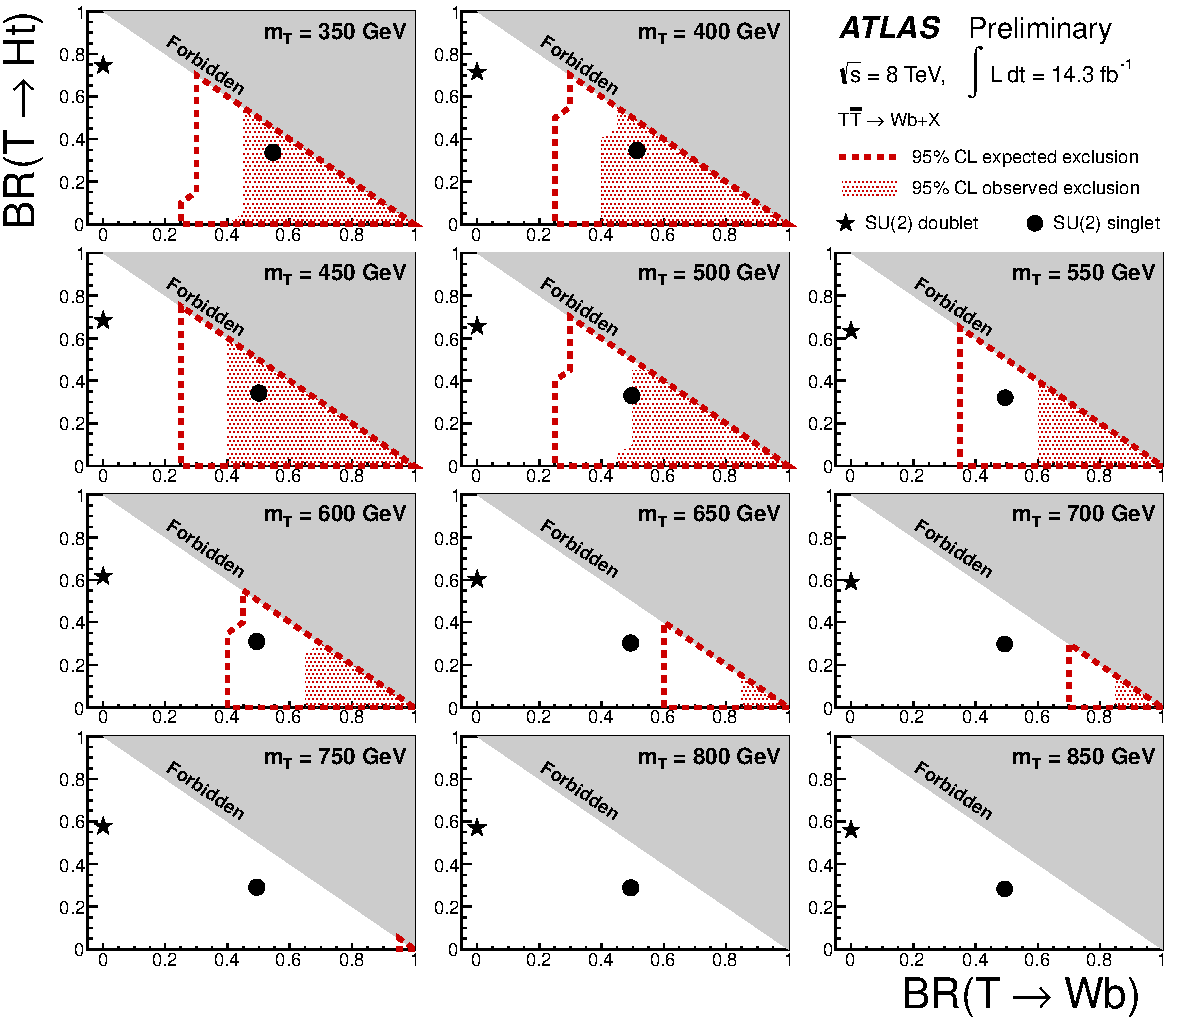
\includegraphics[width=0.7\textwidth]{pics/lim_Scan2D_tight_Bin1.pdf}

\end{frame}





%----------------------------------
\section{Search for \TTbar\ decaying to $Ht+X$}
%----------------------------------
\begin{frame}\frametitle{Strategy}
\centering\myskip

\begin{minipage}{.25\textwidth}\centering
\footnotesize

$\TTbar\to Ht+X$

\myskip

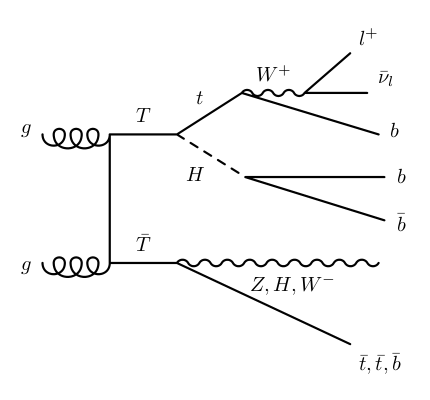
\includegraphics[width=1.15\textwidth]{pics/feyn_htX}

%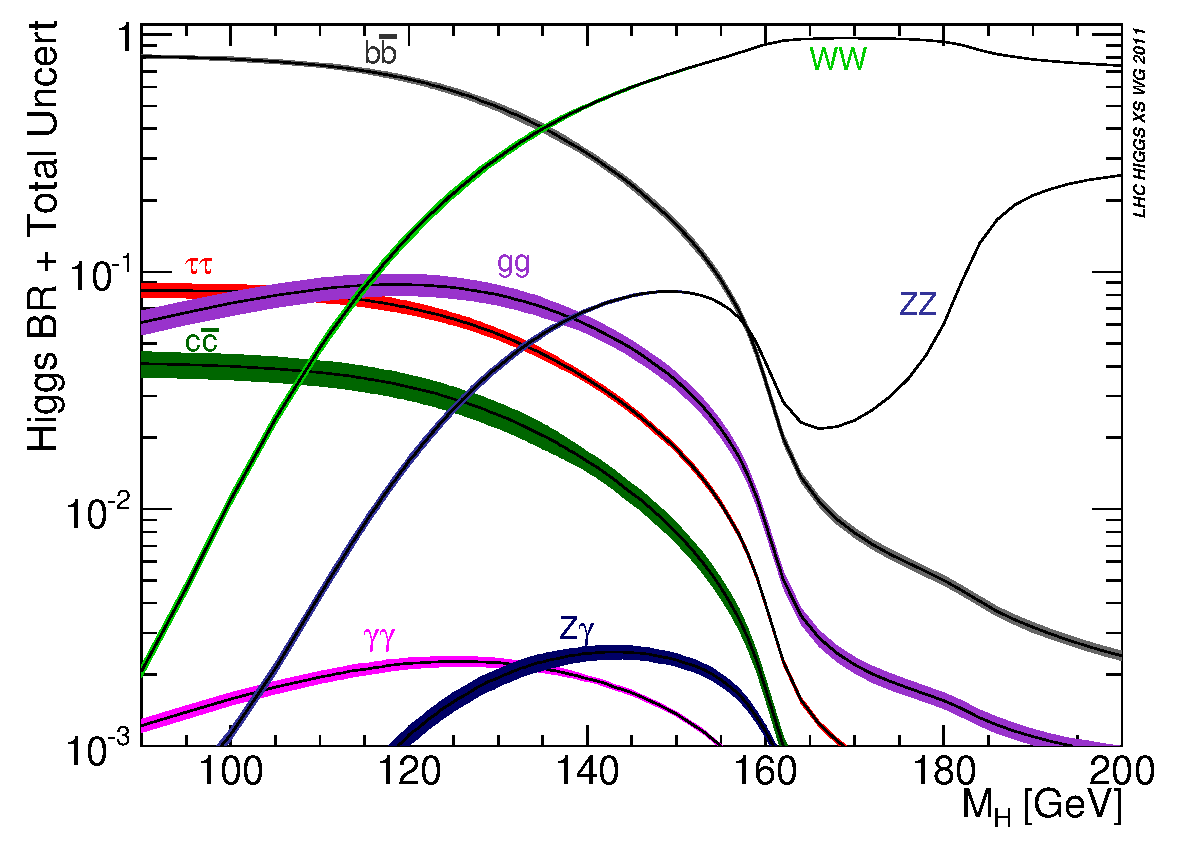
\includegraphics[width=1.15\textwidth]{pics/BRTotalUncertBands_lm}
SM Higgs boson\\
w/ {\cccolor $m_H=125\gev$}\\
$\Downarrow$\\
BR($H\to bb$) = 60\%\\
BR($H\to WW$) = 20\%\\



\end{minipage}\begin{minipage}{.75\textwidth}\centering
\footnotesize
\vskip-5ex

\begin{tabular}{p{.7cm}ll}
  \multirow{2}{*}{$T\to Ht$} & {\tiny$\nearrow$} $bbWb \to bbbl\nu$ & \multirow{2}{*}{+ $\bar{T}\to Wb/Zt/Ht$}\\
                             & {\tiny$\searrow$} $WWWb \to qqqqbl\nu$&\\
\end{tabular}

\myskip

as a minimum {\cccolor 6} total jets in the event ($\TTbar\to HtWb$)\\
{\LARGE $\Downarrow$}\\
$\HT = \pT(l) + \met + \sum_{j = 1}^{\rm N jets}\pT(j)$\\

\scriptsize
\myskip
{\cccolor peak $\sim 2m_T$}\\
good signal/bkg discriminant $\qquad$ for all $Ht+X$ modes


\hskip5ex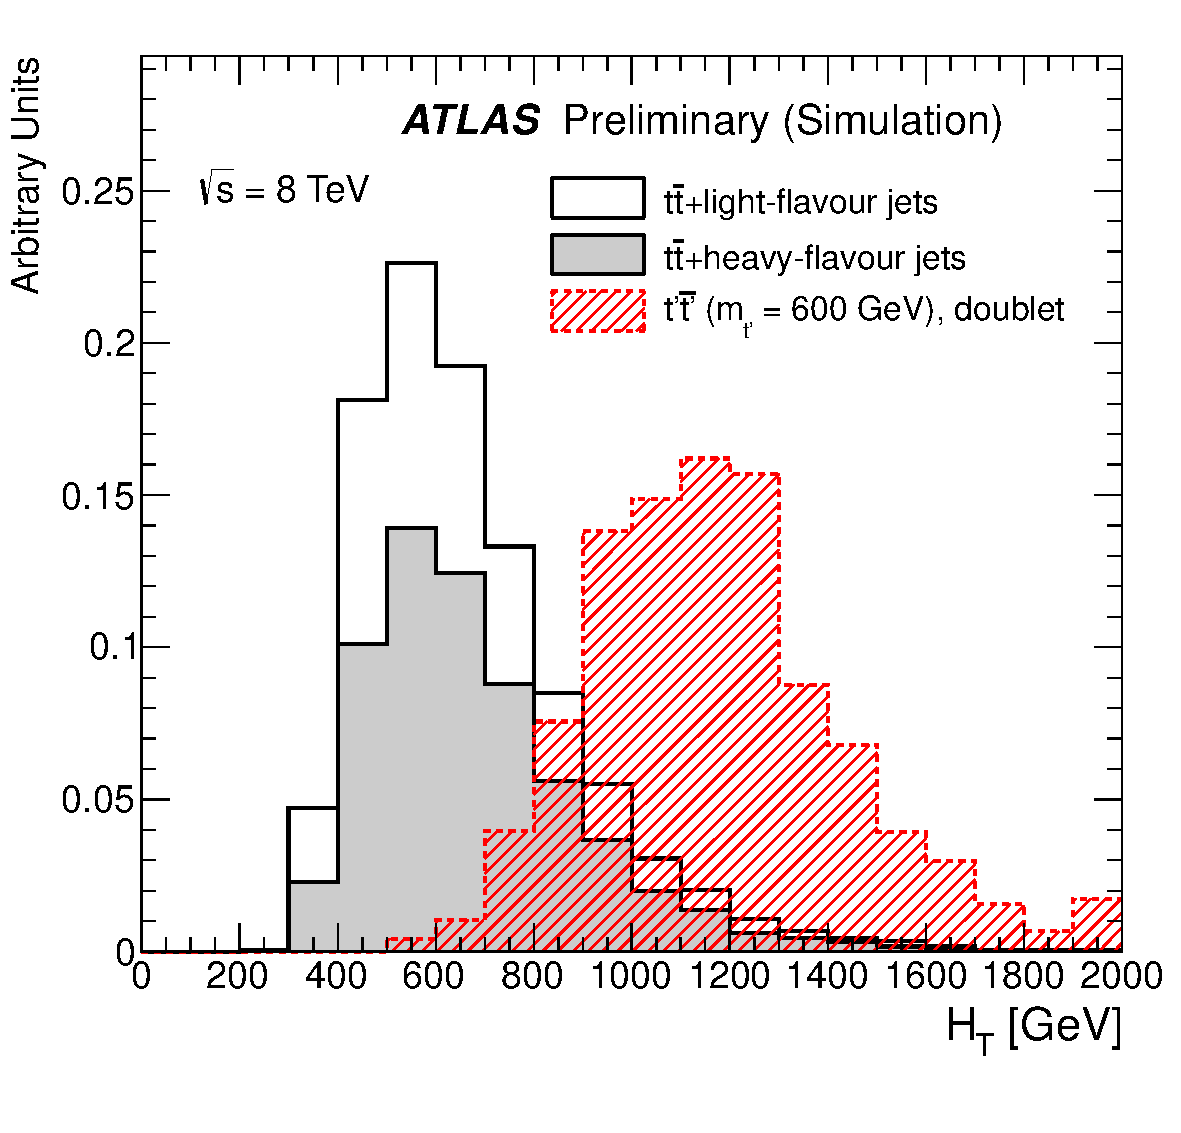
\includegraphics[width=.45\textwidth]{pics/HTAll_ELEMUON_6jetin4btagin_NOMINAL_VLTtt}
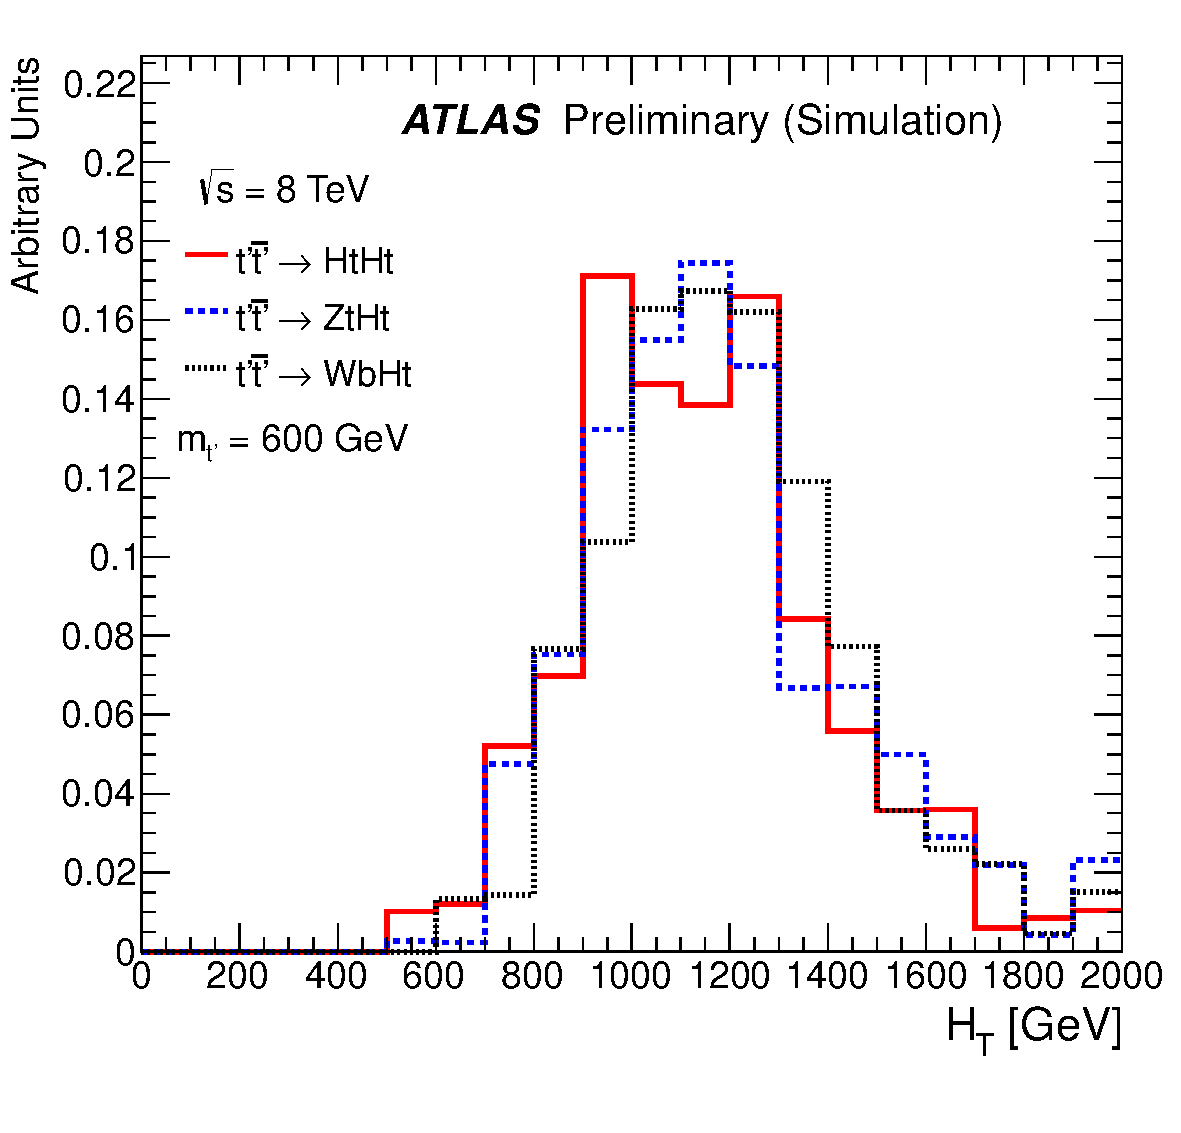
\includegraphics[width=.45\textwidth]{pics/HTAll_ELEMUON_6jetin4btagin_NOMINAL_decaysVLT}

$\geq 6$ jets, $\geq 4$ \bjet s

\end{minipage}

\end{frame}


%%%%%%%%%%%%%%%%%%%%%%%%%
%%%
%%%%%%%%%%%%%%%%%%%%%%%%%
\begin{frame}\frametitle{Event selection}
\centering\footnotesize

\begin{minipage}{.5\textwidth}\centering\scriptsize

\myskip

\begin{tabular}{ll}
\toprule
\pchii\  & $\geq 6$ jets\\
 & =2 $b$-tagged jets \\
 & \cccolor orthogonality cut: \\
 & $\HT < 700~\gev$ \\
\midrule
\pchiii\  & $\geq 6$ jets\\
&  =3 $b$-tagged jets \\
\midrule
\pchiv\  &$\geq 6$ jets\\
& $\geq 4$ $b$-tagged jets \\
\bottomrule
\end{tabular}

\myskip

\end{minipage}\begin{minipage}{.5\textwidth}\centering

%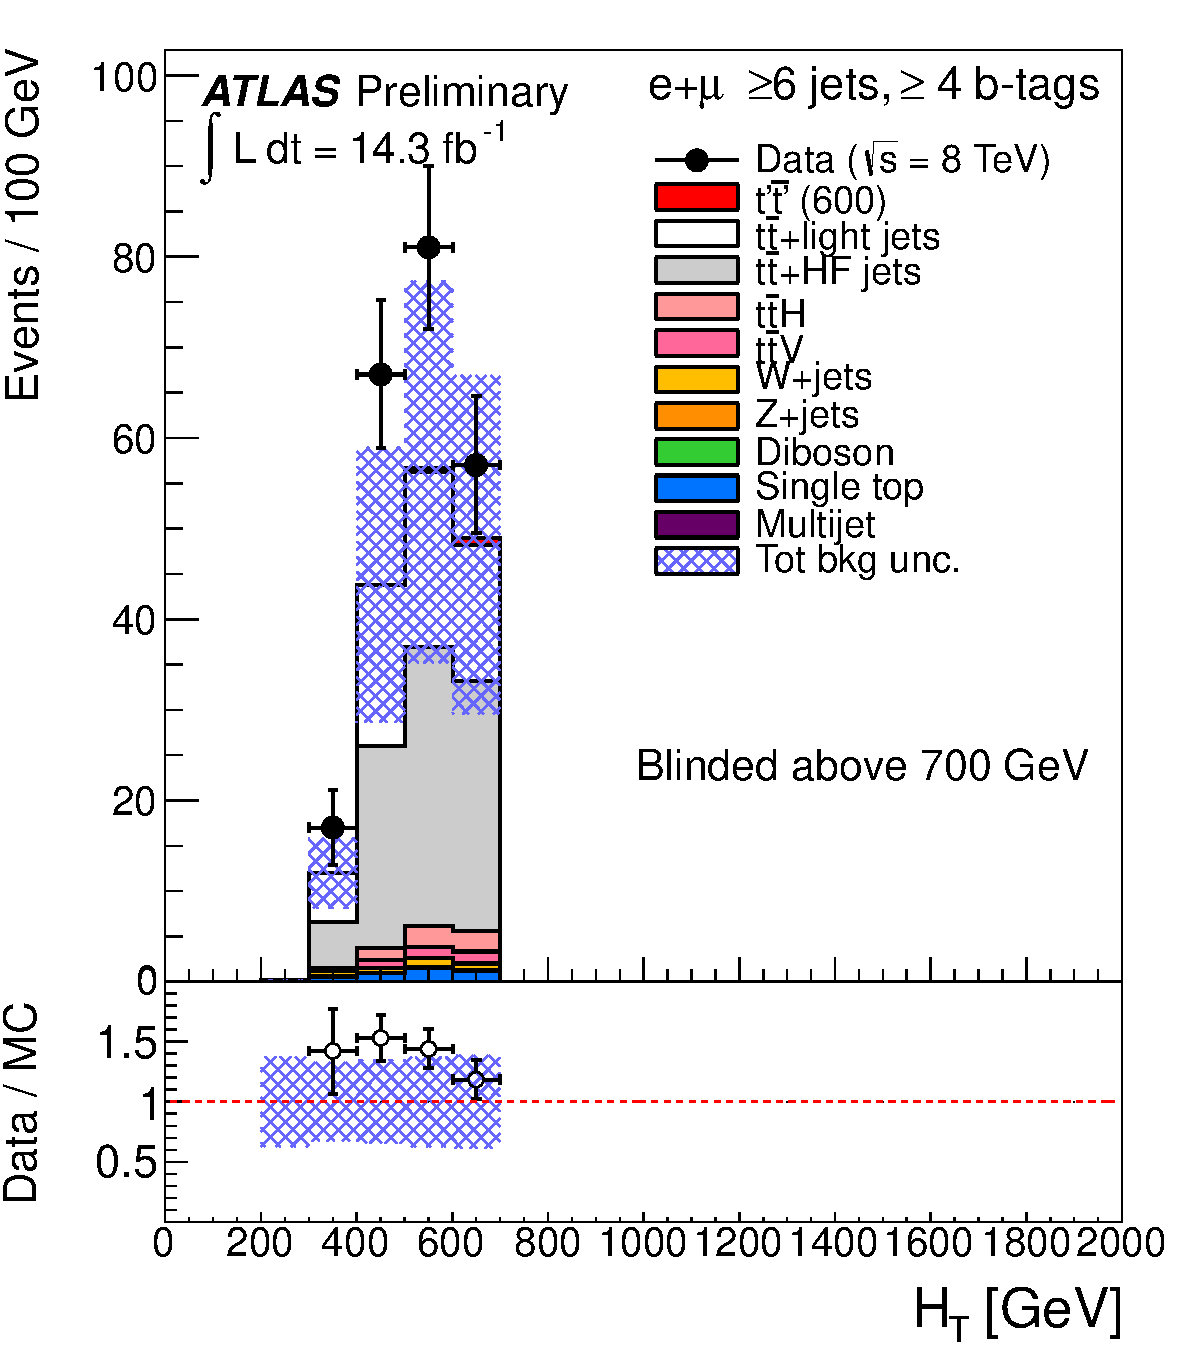
\includegraphics[width=.8\textwidth]{pics/htx_unscaled/HTAll_ELEMUON_6jetin4btagin_NOMINAL.pdf}

Consider three \bjet s multiplicities:
\begin{itemize}
\item maximize signal acceptance
\item insight on the heavy- and light-flavor components
\end{itemize}

each channel has a very different fraction of \tthf\ and \ttlf



\end{minipage}


\end{frame}


%%%%%%%%%%%%%%%%%%%%%%%%%
%%%
%%%%%%%%%%%%%%%%%%%%%%%%%
\begin{frame}\frametitle{Scale of \ttbar\ components}
\centering\footnotesize

use background enriched regions ({\cccolor low \HT}) to correct heavy flavor component \\ 
$\Downarrow$ \\ 
simultaneous fit of \tthf\ and \ttlf\ scaling factors\\
%(good to have {\cccolor background enriched} channels)

 \ttlf: $0.87 \pm 0.02\,{\rm (stat.)} \qquad$  \tthf: $1.35 \pm 0.11\,{\rm (stat.)}$

\myskip
\only<1>{
before\dots\\
\includegraphics[width=.3\textwidth]{pics/htx_unscaled/HTAll_ELEMUON_6jetin2btagex_NOMINAL.pdf}
\includegraphics[width=.3\textwidth]{pics/htx_unscaled/HTAll_ELEMUON_6jetin3btagex_NOMINAL.pdf}
\includegraphics[width=.3\textwidth]{pics/htx_unscaled/HTAll_ELEMUON_6jetin4btagin_NOMINAL.pdf}
}\only<2>{
\dots after\\
\includegraphics[width=.3\textwidth]{pics/htx_scaled/HTAll_ELEMUON_6jetin2btagex_NOMINAL.pdf}
\includegraphics[width=.3\textwidth]{pics/htx_scaled/HTAll_ELEMUON_6jetin3btagex_NOMINAL.pdf}
\includegraphics[width=.3\textwidth]{pics/htx_scaled/HTAll_ELEMUON_6jetin4btagin_NOMINAL.pdf}
%}\only<3>{
%final\\
%\includegraphics[width=.3\textwidth]{pics/htx_final/HTAll_6jetin2btagex_ELEMUON.pdf}
%\includegraphics[width=.3\textwidth]{pics/htx_final/HTAll_6jetin3btagex_ELEMUON.pdf}
%\includegraphics[width=.3\textwidth]{pics/htx_final/HTAll_6jetin4btagin_ELEMUON.pdf}
}

Maximum yields discrepancy below 5\%

\end{frame}


%%%%%%%%%%%%%%%%%%%%%%%%%
%%%
%%%%%%%%%%%%%%%%%%%%%%%%%
\begin{frame}\frametitle{Comparison data vs prediction}
\centering\scriptsize

Blinding cut: $\HT<700\gev$

{\Large$\Downarrow$}

Define special blinded regions to check modeling of high \HT\ tail:

\myskip

at most two jets with $\pt>60\gev$, $\HT<1.2\tev$

\myskip

\begin{minipage}{.45\textwidth}\centering
 2 \btag ged jets\\
\includegraphics[width=.8\textwidth]{pics/htx_httails/HTAll_ELEMUON_6jetin2btagex_NOMINAL_logscale}

\end{minipage}\begin{minipage}{.45\textwidth}\centering

 3 \btag ged jets\\
\includegraphics[width=.8\textwidth]{pics/htx_httails/HTAll_ELEMUON_6jetin3btagex_NOMINAL_logscale}

\end{minipage}

\end{frame}



%%%%%%%%%%%%%%%%%%%%%%%%%
%%%
%%%%%%%%%%%%%%%%%%%%%%%%%
\begin{frame}\frametitle{Most relevant systematic uncertainties}
\centering\footnotesize

\ttbar\ modeling systematics:
\begin{itemize}
\item Assign a 50\% uncertainty on \tthf\ fraction
\item Vary the factorization and renormalization scales in \texttt{ALPGEN}
\end{itemize}

\myskip

{
\scriptsize
\begin{tabular}{l*{4}{c}}\toprule
 & \TTbar & $t\bar{t}$-HF & $t\bar{t}$-Light \\
\midrule
Total [\%]& +21.9/-24.0 & +57.3/-58.4 & +42.0/-44.1 \\
\midrule
\multicolumn{4}{c}{Main contributions [\%]}\\
ttbarHF & -- &+50.0/-50.0 & +13.0/-13.0 \\
ttbar qfac & -- & +0.7/-0.7 & +1.6/-1.6 \\
ttbar iqopt2 & -- & +6.9/-6.9 & +20.1/-20.1 \\
ttbar ktfac & -- & +7.5/-9.2 & +13.8/-17.0 \\
BTAGBREAK8 & +20.4/-22.7 & +15.8/-17.8 & +12.2/-13.1 \\
JES ``baseline'' & +3.1/-3.1 & +10.5/-10.5 & +13.7/-13.7 \\
\bottomrule
\end{tabular}
}

\myskip

Introduce the scaling factors as {\cccolor nuisance parameters}\\
{\Large $\Downarrow$}\\
total uncertainty on background reduced by almost a factor of 2 
%{\cccolor \dots before fitting the nuisance parameters}

\end{frame}


%%%%%%%%%%%%%%%%%%%%%%%%%
%%%
%%%%%%%%%%%%%%%%%%%%%%%%%
\begin{frame}\frametitle{Yields in final regions}
\centering\scriptsize

\myskip
\begin{minipage}{.5\textwidth}\centering

\includegraphics[width=.5\textwidth]{pics/htx_final/HTAll_6jetin2btagex_ELEMUON.pdf}
\includegraphics[width=.5\textwidth]{pics/htx_final/HTAll_6jetin3btagex_ELEMUON.pdf}

%\resizebox{.9\textwidth}{.25\textwidth}{
\resizebox{.9\textwidth}{!}{
\begin{tabular}{l D{;}{\,\pm\,}{-1} D{;}{\,\pm\,}{-1} D{;}{\,\pm\,}{-1}} \toprule
 & \multicolumn{1}{c}{ 2 $b$-tags} & \multicolumn{1}{c}{ 3 $b$-tags} & \multicolumn{1}{c}{ $\geq$ 4 $b$-tags}\\
\midrule
$t\bar{t}$+HF  &  1500;900 &  900;400 &  170;70\\
$t\bar{t}$+LF  &  9600;1000 &  1900;350 &  75;22\\
$W$+jets  &  250;130 &  50;30 &  5;3\\
$Z$+jets  &  50;40 &  9;6 &  0.5;0.9\\
Single top  &  300;70 &  75;18 &  7;3\\
Diboson  &  1.7;0.6 &  0.3;0.1 &  0.03;0.03\\
$t\bar{t}V$ & 70;20 &  36;12 &  7;3\\
$t\bar{t}H$ & 28;4 &  31;6 &  12;3\\
Multijet  &  49;23 &  1.7;0.8 &  0.15;0.06\\
\midrule
Tot.Bkg.  &  11860 ;260 &  2990;210 &  270;60\\
Data & \multicolumn{1}{c}{11885} & \multicolumn{1}{c}{2922} & \multicolumn{1}{c}{318}\\
\midrule
%\multicolumn{7}{l}{Doublet}\\
%\midrule
$T\bar{T}$ (600) & & & \\
doublet &  4.3;1.2 &  94;7 &  79;18\\
singlet  &  2.3;0.4 &  61;7 &  36;9\\
%T\bar{T} (400);550;70 &  1100;100 &  790;160\\
%T\bar{T} (600);4.3;1.2 &  94;7 &  79;18\\
%T\bar{T} (800);0.12;0.05 &  10.7  & 0.8 &  9.1;2.1\\
%\midrule
%\multicolumn{7}{l}{Singlet}\\
%\midrule
%T\bar{T} (400);290;30 &  650;80 &  330;70\\
%T\bar{T} (600);2.3;0.4 &  61;7 &  36;9\\
%T\bar{T} (800);0.06;0.01 &  6.9;0.7 &  4.2;1.1\\
\bottomrule
\end{tabular}
}

\myskip

\footnotesize

\end{minipage}\begin{minipage}{.5\textwidth}\centering

\includegraphics[width=.9\textwidth]{pics/htx_final/HTAll_6jetin4btagin_ELEMUON}

\end{minipage}

\end{frame}


%%%%%%%%%%%%%%%%%%%%%%%%%
%%%
%%%%%%%%%%%%%%%%%%%%%%%%%
\begin{frame}\frametitle{Benchmark results}
\centering\footnotesize

\begin{minipage}{.5\textwidth}\centering

Doublet\\

\includegraphics[width=0.9\textwidth]{pics/lim_doublet}\\

observed (expected) 95\%  CL limit $m_{T}>790\,(745)\gev$

\end{minipage}\begin{minipage}{.5\textwidth}\centering

Singlet\\

\includegraphics[width=0.9\textwidth]{pics/lim_singlet}\\

observed (expected) 95\%  CL  limit  $m_{\T}>640\,(615)\gev$

\end{minipage}

\end{frame}

%%%%%%%%%%%%%%%%%%%%%%%%%
%%%
%%%%%%%%%%%%%%%%%%%%%%%%%
\begin{frame}\frametitle{Model independent results}
\centering\footnotesize

\includegraphics[width=0.7\textwidth]{pics/lim_2D}

\end{frame}





%----------------------------------
\section{Combined results}
%----------------------------------

%%%%%%%%%%%%%%%%%%%%%%%%%
%%%
%%%%%%%%%%%%%%%%%%%%%%%%%
\begin{frame}\frametitle{Combination of \wbx\ and \htx}
\centering\footnotesize

\begin{minipage}{.5\textwidth}\centering
\includegraphics[width=.5\textwidth]{pics/combo/HTAll_6jetin2btagex_ELEMUON}
\includegraphics[width=.5\textwidth]{pics/combo/HTAll_6jetin3btagex_ELEMUON}\\
\includegraphics[width=.5\textwidth]{pics/combo/HTAll_6jetin4btagin_ELEMUON}
\includegraphics[width=.5\textwidth]{pics/combo/VLQAna_WbX_1W_MWb_4_ELEMUON_cutflow1234567_NOMINAL}

\end{minipage}\begin{minipage}{.5\textwidth}\centering
\myskip

The searches are orthogonal\\
$\Downarrow$\\
can be combined in the statistical analysis\\
(consistent {\cccolor syst unc} treatment)

\includegraphics[width=.9\textwidth]{pics/combo/lim_singlet_comb.pdf}

\end{minipage}

\end{frame}



%%%%%%%%%%%%%%%%%%%%%%%%%
%%%
%%%%%%%%%%%%%%%%%%%%%%%%%
\begin{frame}\frametitle{Results}
\centering\footnotesize

\begin{minipage}{.3\textwidth}\centering

aaaa
\end{minipage}\begin{minipage}{.7\textwidth}\centering

\begin{pgfpicture}{0.0\textwidth}{0.0\textheight}{1.\textwidth}{.6\textwidth}
   \begin{pgftranslate}{\pgfpoint{0.0\textwidth}{-0.15\textheight}}
\pgfdeclareimage[interpolate=true,width=1.\textwidth]{wbx}{pics/lim_Scan2D_tight_Bin1.pdf}
\pgfdeclareimage[interpolate=true,width=1.\textwidth]{htx}{pics/combo/htxT.png}
\pgfdeclareimage[interpolate=true,width=1.\textwidth]{comb}{pics/combo/combT.png}
\pgfdeclareimage[interpolate=true,width=1.\textwidth]{br2d}{pics/combo/lim_Scan2D_comb.pdf}
%\pgfputat{\pgfxy(0.0,0.0)}{\pgfbox[left,base]{\pgfuseimage{mindr}}}
 \pgfsetlinewidth{1.pt}
 \usebeamercolor[bg]{head/foot boxes}
\pgfputat{\pgfxy(0.0,0.0)}{\pgfbox[left,base]{\pgfuseimage{wbx}}}
\onslide<2->{
\pgfputat{\pgfxy(0.0,0.0)}{\pgfbox[left,base]{\pgfuseimage{htx}}}
}
\onslide<3->{
\pgfputat{\pgfxy(0.0,0.0)}{\pgfbox[left,base]{\pgfuseimage{comb}}}
}
\onslide<4->{
\pgfputat{\pgfxy(0.0,0.0)}{\pgfbox[left,base]{\pgfuseimage{br2d}}}
}
   \end{pgftranslate}

\end{pgfpicture}

\end{minipage}


\end{frame}

\FullBackgroundPicture{pics/ATLAS_VLQ_TT_june2013_step4}
%%%%%%%%%%%%%%%%%%%%%%%%%
%%%
%%%%%%%%%%%%%%%%%%%%%%%%%
\begin{frame}\frametitle{ATLAS BR coverage}
\centering\footnotesize

%\includegraphics[width=0.8\textwidth]{pics/ATLAS_VLQ_TT_june2013_step4}

\end{frame}


\FullBackgroundPicture{pics/ATLAS_VLQ_BB_june2013_step2}
%%%%%%%%%%%%%%%%%%%%%%%%%
%%%
%%%%%%%%%%%%%%%%%%%%%%%%%
\begin{frame}\frametitle{ATLAS BR coverage}
\centering\footnotesize

%\includegraphics[width=0.8\textwidth]{pics/ATLAS_VLQ_BB_june2013_step2}

\end{frame}


\FullBackgroundPicture{pics/emptyIMG}
%%%%%%%%%%%%%%%%%%%%%%%%%
%%%
%%%%%%%%%%%%%%%%%%%%%%%%%
\begin{frame}\frametitle{Comparison to CMS results}
\centering\footnotesize

Inclusive \TTbar\ searches {\cccolor CMS-PAS-B2G-12-015~\cite{CMS-PAS-B2G-12-015}}
\myskip

\begin{minipage}{.6\textwidth}
\includegraphics[width=.8\textwidth]{pics/cms/triangle}
\end{minipage}\begin{minipage}{.4\textwidth}\centering

\begin{pgfpicture}{0.0\textwidth}{0.0\textheight}{1.\textwidth}{.6\textwidth}
   \begin{pgftranslate}{\pgfpoint{-0.05\textwidth}{-0.15\textheight}}
\pgfdeclareimage[interpolate=true,width=1.\textwidth]{tabTT}{pics/cms/tableTT}
 \pgfsetlinewidth{1.pt}
 \usebeamercolor[bg]{head/foot boxes}
 \pgfputat{\pgfxy(0.0,0.0)}{\pgfbox[left,base]{\pgfuseimage{tabTT}}}
 \pgfrect[stroke]{\pgfxy(0.2,3.4)}{\pgfxy(5,0.25)}
 \pgfputat{\pgfxy(-1.2,3.4)}{\pgfbox[left,base]{\cccolor ``doublet''}}
 \pgfputat{\pgfxy(-1.2,3.1)}{\pgfbox[left,base]{\cccolor 790 obs}}
 \pgfrect[stroke]{\pgfxy(0.2,1.4)}{\pgfxy(5,0.25)}
 \pgfputat{\pgfxy(-1.2,1.4)}{\pgfbox[left,base]{\cccolor ``singlet''}}
 \pgfputat{\pgfxy(-1.2,1.1)}{\pgfbox[left,base]{\cccolor 670 obs}}
 \pgfrect[stroke]{\pgfxy(0.2,0.)}{\pgfxy(5,0.25)}
 \pgfputat{\pgfxy(-1.2,0.)}{\pgfbox[left,base]{\cccolor ``chiral''}}
 \pgfputat{\pgfxy(-1.2,-0.3)}{\pgfbox[left,base]{\cccolor 740 obs}}
 \pgfrect[stroke]{\pgfxy(4,-0.05)}{\pgfxy(1,5.)}
\end{pgftranslate}
\end{pgfpicture}

\end{minipage}


\end{frame}





%----------------------------------
\section{Conclusions and outlook}
%----------------------------------

\begin{frame}\frametitle{Conclusions and outlook}
\footnotesize\centering

{\it both searches are being updated with the full {\cccolor 20~\ifb} statistics}

\begin{minipage}{.3\textwidth}\centering
\includegraphics[width=.8\textwidth]{pics/VLQAna_WbX_1W_MWb_4_ELEMUON_cutflow1234567_NOMINAL.pdf}
\end{minipage}\begin{minipage}{.7\textwidth}\centering
\begin{tabular}{l}
\buuu poor MC bkgs statistical population in the \tight\ channel\\
\\
\yeee {\cccolor larger MC samples} available\\
\yeee possible optimization of the {\cccolor\htfj\ cut}\\
\yeee explorable option: larger anti-$k_{t}$ {\cccolor jets}\\
\end{tabular}

\myskip
Best up-to-date 95\% CL obs limit on \\
chiral $T$ and vector-like $Y$ (740~\gev)

\end{minipage}

\begin{minipage}{.7\textwidth}\centering
\begin{tabular}{l}
\buuu poor modeling of \tthf\ by \texttt{ALPGEN}\\
\buuu \btag ging calibration sub-optimal for\\
\phantom{\buuu} analyses with high-\pt\ objects\\
\\
\yeee {\cccolor\ttbar-based} calibrations being developed\\
\yeee potential high gain in sensitivity with {\cccolor profiling}\\
\yeee easily optimizable for a {\cccolor$B\bar{B}\to Hb+X$} analysis\\
\end{tabular}

\myskip
Best up-to-date 95\% CL obs limit on doublet $T$

\end{minipage}\begin{minipage}{.3\textwidth}\centering
\includegraphics[width=.8\textwidth]{pics/htx_final/HTAll_6jetin4btagin_ELEMUON.pdf}
\end{minipage}

\end{frame}

\begin{frame}\frametitle{Outlook}
\small\centering

\begin{minipage}{.7\textwidth}\centering

{\it all four} ATLAS searches are being updated\\ with the full {\cccolor 20~\ifb} statistics,\\ plus two new channels: $B\bar{B}\to Wt+X$ and $B\bar{B}\to Hb+X$

\end{minipage}

\myskip

\begin{minipage}{.6\textwidth}\centering
LHC Run-II: \\
\myskip
\begin{tabular}{l}
\yeee \rts=14~\tev\\
\yeee $\sim 100\ifb$ in 3 years\\
\buuu higher pile-up\\
\end{tabular}


\myskip

To-do:\\
\begin{itemize}
\item continue on the road of full combination
\item design searches for single production
\end{itemize}

\myskip

\begin{flushright}\scriptsize
plots from~\cite{Aguilar-Saavedra:2013qpa}
\end{flushright}

\end{minipage}\begin{minipage}{.4\textwidth}\centering
\includegraphics[width=.85\textwidth]{pics/ja/fig4a}\\
\includegraphics[width=.85\textwidth]{pics/ja/fig4b}
\end{minipage}

\end{frame}


\begin{frame}\frametitle{Thank you!}
\large\centering


Thank you for your attention!

\myskip

\includegraphics[width=.5\textwidth]{pics/boooks.jpg}

\end{frame}


\appendix


\section*{References}
\setbeamertemplate{bibliography item}[text]

\begin{frame}[allowframebreaks]
\frametitle{References}\footnotesize
\bibliographystyle{unsrt}
%\bibliographystyle{myunsrt}
\bibliography{../bibliography/biblio}
\end{frame}


\section*{Backup}

%----------------------------------
\begin{frame}
 \frametitle{}

\begin{center}{\bfseries
BACKUP SLIDES}
\end{center}
\end{frame}


\begin{frame}\frametitle{LHC parameters}
\footnotesize\centering\myskip
\begin{table}\centering
	\begin{tabular}{lllll}\toprule
        Parameter                       & designed      &       2010 &  2011     &   2012\\ \midrule
        Beam energy (\tev/c)            & 7             & 3.5        & 3.5       & 4    \\
        Beta function $\beta*$ (m)      & 0.55          & 2.0/3.5    & 1.5/1.0   & 0.6  \\
        Max. No. bunches/beam           & 2808          & 368        & 1380      &1380  \\
        Max. No. protons/bunch          & 1.15$\times10^{11}$ & 1.2$\times10^{11}$ & 1.45$\times10^{11}$ & 1.7$\times10^{11}$ \\
        Bunch spacing (ns)              & 25            & 150       & 75/50        & 50 \\
        Peak luminosity (\cmm2\sm1)     & 1$\times10^{34}$& 2.1$\times10^{32}$& 3.7$\times10^{33}$& 7.7$\times10^{33}$\\
        Emittance $\varepsilon_{n}$ ($\mu$rad)&3.75     &   2.0      & 2.4      & 2.5   \\
        Max. $<\mu>$                    & 19            & 4             & 17         & 37       \\
	\bottomrule\end{tabular}\caption{Overview of some parameters for the LHC performance comparing the design values with their time
        evolution during the first long run operation in 2010-2013~\cite{Lamont}.}\label{tab:lhcpar}
\end{table}

\end{frame}








\begin{frame}\frametitle{\wbx\ 7~\tev\ vs 8~\tev}
\footnotesize\centering

\begin{table}[!htb]
\begin{center}\small
\begin{tabular}{p{3cm}cc}
\toprule
Selection & 7~\tev & 8~\tev \\
\midrule
%\multirow{10}{*}{Preselection} & \multicolumn{2}{c}{One electron or muon$^{(*)}$}  \\\cmidrule{2-3}
\ldelim\{{12}{12ex}[\hskip4ex Preselection] & \multicolumn{2}{c}{One electron or muon$^{(+)}$}  \\\cmidrule{2-3}
             & $\met >35(20)\gev$ for electron & $\met >20\gev$ \\
             &  (muon) channel & \\\cmidrule{2-3}
             & \multicolumn{2}{c}{$\met +m_{\rm T}>60\gev$} \\\cmidrule{2-3}
             & $\geq 3$ jets for \wi & \multirow{2}{*}{$\geq 4$ jets$^{(*)}$}\\
             & $\geq 4$ jets for \wii & \\\cmidrule{2-3}
             & \multicolumn{2}{c}{$\geq 1$ $b$-tagged jets$^{(**)}$} \\\cmidrule{2-3}
             & & orthogonality cut:\\
             & & reject events with $\geq 6$ jets \\
             & & and $\geq 3$ $b$-tagged jets \\
\midrule
%\end{tabular}
%\begin{tabular}{lll}
%\multirow{6}{*}{\loose\ selection} & \multicolumn{2}{c}{ Preselection } \\
\ldelim\{{6}{6ex}[\loose\ selection] & \multicolumn{2}{c}{ Preselection } \\
                  & \multicolumn{2}{c}{$\geq 1~W_{\rm had}$ candidates$^{(\rm x)}$} \\
                  & $\htfj>750\gev$ & $\htfj>800\gev$ \\
                  & \multicolumn{2}{c}{ $\pt(b_1) > 160\gev$}\\
                  & $\pt(b_2) >60\gev$ & $\pt(b_2) >80\gev$ \\
                  & $\Delta R(\ell,\nu)<1.4$ & $\Delta R(\ell,\nu)<1.2$ \\
\midrule
%\multirow{3}{*}{\tight\  selection} & \multicolumn{2}{c}{ \loose\ selection} \\
\ldelim\{{3}{3ex}[\tight\  selection] & \multicolumn{2}{c}{ \loose\ selection} \\
     	      & \multicolumn{2}{c}{ min$\Delta R(\ell,b)>1.4$}\\
              & \multicolumn{2}{c}{ min$\Delta R(W_{\rm had},b)>1.4$} \\
\bottomrule
\multicolumn{3}{c}{\footnotesize (+) Leptons have different $p_T$ thresholds and triggers. Both follow {\it topcommon} prescriptions.}\\
\multicolumn{3}{c}{\footnotesize (*) Jets in 7\tev\ (8\tev) analyses are calibrated at the EM+JES (LC+JES) scale.}\\
\multicolumn{3}{c}{\footnotesize (*) The $b$-tagging algorithm and working point for 7\tev\ and 8\tev analyses are the same: MV1, 70\%.}\\
\multicolumn{3}{c}{\footnotesize (x) The boosted $W$ reconstruction for 7\tev\ and 8\tev analyses is slightly different, see text.}\\
\bottomrule
\end{tabular}
\caption{Comparison of event selection requirements for the 7~\tev\ and 8~\tev analyses.}
\label{tab:wbx7tevselection}
\end{center}
\end{table}

\end{frame}


%%%%%%%%%%%%%%%%%%%%%%%%%
%%%
%%%%%%%%%%%%%%%%%%%%%%%%%
\begin{frame}\frametitle{Neutrino reconstruction}
\centering\footnotesize

Neutrino 4-momentum unknown \\
{\large $\Downarrow$}\\
$\met$ $X$ and $Y$ components + a bit of algebra:\\
$(P_l + P_{\nu})^2 = P_W^2 = M_W^2$\\
{\large $\Downarrow$}\\
two possible $p_{Z_\nu}$ solutions for the 
$Z$ component of the neutrino momentum:\\
$p_{Z_\nu} = \dfrac{\lambda \pm \sqrt{\delta} }{2}$\\

\myskip
Choose the solution giving min$|m_{\rm reco}^{\rm had} - m_{\rm reco}^{\rm lep}|$\\
(this implies also \bjet s association!)

\begin{itemize}
\item If no real solution, $\nu\sim$ collinear to $l \Rightarrow$  $\eta_{\nu}$ set equal to $\eta_{l}$
\end{itemize}

\begin{minipage}{.5\textwidth}\centering
{\scriptsize
\begin{eqnarray*}
\lambda &=& 2\beta \dfrac{p_{Z_l}}{E_l^2-p_{Z_l}^2};\\
\delta  &=& \lambda^2 - 4\gamma;\\
\gamma &=& -\dfrac{\beta^2 - E_l^2 (p_{X_\nu}^2+p_{Y_\nu}^2)}{E_l^2-p_{Z_l}^2}; \\
\end{eqnarray*}
}
\end{minipage}\begin{minipage}{.5\textwidth}\centering
{\scriptsize
\begin{eqnarray*}
\beta  &=& \alpha + p_{X_\nu}p_{X_l} + p_{Y_\nu}p_{Y_l}; \\
\alpha &=& \dfrac{1}{2}(M_W^2 - M_l^2).
\end{eqnarray*}
}
\end{minipage}

\end{frame}



%%%%%%%%%%%%%%%%%%%%%%%%%
%%%
%%%%%%%%%%%%%%%%%%%%%%%%%
\begin{frame}\frametitle{Statistical analyses}
\centering\footnotesize

In the 7~\tev\ analysis three configurations have been tested:

\begin{itemize}
\item \loose\ selection using
$m_{\rm reco}$ and profiling of overall $t\bar{t}$ yield (``\loose'')
\item \tight\ selection 
using $m_{\rm reco}$ (``\tight'')
\item \tight\ selection  considering just the overall yield and not 
the shape of $m_{\rm reco}$ (``\tight\ cut-and-count'')
\end{itemize} 

Look at expected value of $CL_{\rm s}$ as a function of $m_{\T}$ for best performance:\\

\includegraphics[width=.6\textwidth]{pics/CLs_versus_Mass}


\end{frame}



%%%%%%%%%%%%%%%%%%%%%%%%%
%%%
%%%%%%%%%%%%%%%%%%%%%%%%%
\begin{frame}\frametitle{Generator choice for \ttbar}
\centering\footnotesize

Comparison data to background prediction w/ different \ttbar\ generators\\
e.g. in SDR3 ({\sl loose} selection with reversed $b$-jet $\pt$ cuts)\\
\myskip

\begin{minipage}{.33\textwidth}\centering
\texttt{MC@NLO}\\
\includegraphics[width=0.9\textwidth]{pics/wbxgen/ttbar5200/VLQAna_WbX_MinDRlb_ELEMUONCR2_1W_NOMINAL}

\end{minipage}\begin{minipage}{.33\textwidth}\centering
\texttt{POWHEG+PYTHIA} \\
\includegraphics[width=0.9\textwidth]{pics/wbxgen/ttbar117050/VLQAna_WbX_MinDRlb_ELEMUONCR2_1W_NOMINAL}


\end{minipage}\begin{minipage}{.33\textwidth}\centering
\texttt{ALPGEN+HERWIG}\\
\includegraphics[width=0.9\textwidth]{pics/wbxgen/ttbarAlpgen_HFOR/VLQAna_WbX_MinDRlb_ELEMUONCR2_1W_NOMINAL}


\end{minipage}


\end{frame}


%%%%%%%%%%%%%%%%%%%%%%%%%
%%%
%%%%%%%%%%%%%%%%%%%%%%%%%
\begin{frame}\frametitle{\ttbar\ modeling systematic uncertainties}
\centering\footnotesize

\includegraphics[width=.33\textwidth]{pics/GEN_RATIO.pdf}
\includegraphics[width=.33\textwidth]{pics/FRAG_RATIO.pdf}
\includegraphics[width=.33\textwidth]{pics/PS_RATIO.pdf}

\end{frame}




\begin{frame}\frametitle{Doublet vs singlet}
\centering\myskip\scriptsize

MC simulated for {\cccolor singlet \T} with BR = 1/3 for
every decay mode

\begin{itemize}
\item Mixing between SM quarks and \T\ is {\cccolor left-handed} for singlets, {\cccolor right-handed} for doublets
\end{itemize}

\includegraphics[width=0.45\textwidth]{pics/doubletcomp_HTAll_ELEMUON_6jetin3btagex_NOMINAL}
\includegraphics[width=0.45\textwidth]{pics/doubletcomp_HTAll_ELEMUON_6jetin4btagin_NOMINAL}

Discrepancies in yields below 5\% in \pchiv

\end{frame}



%%%%%%%%%%%%%%%%%%%%%%%%%
%%%
%%%%%%%%%%%%%%%%%%%%%%%%%
\begin{frame}\frametitle{Most relevant systematic uncertainties}
\centering\footnotesize


\resizebox{1.\textwidth}{!}{
\begin{tabular}{l*{10}{c}}
\toprule
 & \TTbar & $t\bar{t}$H (125) & $t\bar{t}$-HF & $t\bar{t}$-Light & $W$+jets & $Z$+jets & Single top & Diboson & $t\bar{t}$$V$ & Multijet\\
\midrule
Total [\%]& +21.9/-24.0 & +25.2/-30.0 & +57.3/-58.4 & +42.0/-44.1 & +60.0/-61.0 & +65.2/-66.2 & +31.7/-32.9 & +68.2/-70.2 & +37.6/-38.8 & +50.0/-50.0\\
\midrule
\multicolumn{10}{c}{Main contributions [\%]}\\
BTAGBREAK8 & +20.4/-22.7 & +18.7/-21.6 & +15.8/-17.8 & +12.2/-13.1 & +13.5/-15.0 & +13.0/-13.9 & +15.9/-17.8 & +22.0/-27.4 & +16.4/-18.6 & --\\
JES ``baseline'' & +3.1/-3.1 & +7.3/-7.3 & +10.5/-10.5 & +13.7/-13.7 & +18.1/-18.1 & +18.2/-18.2 & +19.9/-19.9 & +5.2/-5.2 & +8.4/-8.4 & --\\
ttbar iqopt2 & -- & -- & +6.9/-6.9 & +20.1/-20.1 & -- & -- & -- & -- & -- & --\\
ttbar ktfac & -- & -- & +7.5/-9.2 & +13.8/-17.0 & -- & -- & -- & -- & -- & --\\
ttbar qfac & -- & -- & +0.7/-0.7 & +1.6/-1.6 & -- & -- & -- & -- & -- & --\\
ttbarHF & -- & -- & +50.0/-50.0 & +13.0/-13.0 & -- & -- & -- & -- & -- & --\\
\bottomrule
\end{tabular}
}

\includegraphics[width=.33\textwidth]{pics/6jetin4btagin_ELEMUON_ttbar-HF_JESBREAK1}
\includegraphics[width=.33\textwidth]{pics/6jetin4btagin_ELEMUON_ttbar-Light_JESBREAK1}


\end{frame}




\begin{frame}\frametitle{Treatment of sys unc in combination}
\centering\myskip\scriptsize

\resizebox{1.\textwidth}{!}{
\begin{tabular}{llcccc}
\toprule
& Systematic uncertainty & \multicolumn{2}{c}{ \wbx\  } & \multicolumn{2}{c}{ \htx\  }\\
& & Status  & Components & Status  & Components\\
\midrule
\ldelim\{{16}{16ex}[Fully Correlated] &Luminosity &  N & 1 &  N & 1\\
& Lepton ID+reco+trigger      &  N & 1 &  N & 1\\
& Jet vertex fraction efficiency & SN & 1 & SN & 1\\
& Jet energy resolution       & SN & 1 & SN & 1\\
& $b$-tagging efficiency      & SN & 9 & SN & 9\\
& $c$-tagging efficiency      & SN & 5 & SN & 5\\
& Light jet-tagging efficiency    & SN & 1 & SN & 1\\
& $t\bar{t}$ cross section    &  N & 1 &  N & 1\\
& $t\bar{t}V$ cross section   &  N & 1 &  N & 1\\
& $t\bar{t}H$ cross section   & - & - &  N & 1\\
& Single top cross section    &  N & 1 &  N & 1\\
& Dibosons cross section      &  N & 1 &  N & 1\\
& $W$+jets normalization      &  N & 5 &  - & -\\
& $Z$+jets normalization      &  N & 1 &  - & -\\
& $V$+jets normalization      &  - & - &  N & 1\\
& Multijet normalization      &  - & - &  N & 1\\
\ldelim\{{3}{3ex}[\hskip3ex Uncorrelated]& $t\bar{t}$ modelling        & SN & 3 & SN & 3\\
& $V$+jets modelling         & SN & 1 &  - & -\\
& $t\bar{t}$+heavy-flavour fractions &  - & -& N & 1\\
Correlate & \\
JES w/ BASELINE & Jet energy scale            & SN & 1 & SN & 8\\
\bottomrule
\end{tabular}
}

\end{frame}


%%%%%%%%%%%%%%%%%%%%%%%%%
%%%
%%%%%%%%%%%%%%%%%%%%%%%%%
\begin{frame}\frametitle{Comparison to CMS results}
\centering\footnotesize

Inclusive \TTbar\ searches {\cccolor CMS-PAS-B2G-12-015~\cite{CMS-PAS-B2G-12-015}}
\myskip

\begin{minipage}{.6\textwidth}
\includegraphics[width=.8\textwidth]{pics/cms/triangle}
\end{minipage}\begin{minipage}{.4\textwidth}\centering

\begin{pgfpicture}{0.0\textwidth}{0.0\textheight}{1.\textwidth}{.6\textwidth}
   \begin{pgftranslate}{\pgfpoint{-0.05\textwidth}{-0.15\textheight}}
\pgfdeclareimage[interpolate=true,width=1.\textwidth]{tabTT}{pics/cms/tableTT}
 \pgfsetlinewidth{1.pt}
 \usebeamercolor[bg]{head/foot boxes}
 \pgfputat{\pgfxy(0.0,0.0)}{\pgfbox[left,base]{\pgfuseimage{tabTT}}}
 \pgfrect[stroke]{\pgfxy(0.2,3.4)}{\pgfxy(5,0.25)}
 \pgfputat{\pgfxy(-1.2,3.4)}{\pgfbox[left,base]{\cccolor ``doublet''}}
 \pgfputat{\pgfxy(-1.2,3.1)}{\pgfbox[left,base]{\cccolor 790 obs}}
 \pgfrect[stroke]{\pgfxy(0.2,1.4)}{\pgfxy(5,0.25)}
 \pgfputat{\pgfxy(-1.2,1.4)}{\pgfbox[left,base]{\cccolor ``singlet''}}
 \pgfputat{\pgfxy(-1.2,1.1)}{\pgfbox[left,base]{\cccolor 670 obs}}
 \pgfrect[stroke]{\pgfxy(0.2,0.)}{\pgfxy(5,0.25)}
 \pgfputat{\pgfxy(-1.2,0.)}{\pgfbox[left,base]{\cccolor ``chiral''}}
 \pgfputat{\pgfxy(-1.2,-0.3)}{\pgfbox[left,base]{\cccolor 740 obs}}
 \pgfrect[stroke]{\pgfxy(4,-0.05)}{\pgfxy(1,5.)}
\end{pgftranslate}
\end{pgfpicture}

\end{minipage}


\end{frame}



\end{document}
